% \vspace{0.1cm}  % 添加0.1厘米的垂直空间
% 
% \begin{table}[h]  % 开始表格环境,h表示尽量将表格放在当前位置
% 	\renewcommand{\arraystretch}{1.5}  % 设置表格行距为1.5倍
% 	\centering  % 表格居中
% 	\bicaption[\xiaosi 电流类型对效率的影响]{\wuhao 电流类型对效率的影响}{\wuhao Current type impact on efficiency}  % 双语标题,方括号内是目录中显示的标题(小四号字),第一个花括号内是中文标题(五号字),第二个花括号内是英文标题(五号字)
% 	\begin{tabular}{p{3cm}p{3cm}p{3cm}p{3cm}}  % 开始表格内容,定义4列,每列宽度为3厘米,p表示允许文本自动换行
% 		\toprule[1.5pt]  % 顶部粗线,粗细为1.5pt
% 		\makecell[c]{\songti\wuhao 电流类型}&\makecell[c]{\songti\wuhao A}&\makecell[c]{\songti\wuhao B}&\makecell[c]{\songti\wuhao C}\\  % 表头行,\makecell[c]表示单元格内容居中,\songti表示宋体,\wuhao表示五号字
% 		\hline  % 普通横线
% 		\makecell[c]{\wuhao aaa}&\makecell[c]{\wuhao aa1}&\makecell[c]{\wuhao bb1}&\makecell[c]{\wuhao cc1}\\  % 数据行,格式同上
% 		\bottomrule[1.5pt]  % 底部粗线,粗细为1.5pt
% 	\end{tabular}
%    \label{tab:3.1}  % 表格标签,用于交叉引用	
% \end{table}
%
% \vspace{-0.1cm}  % 调整表格与下文的间距




\begin{table}
	\centering
	\bicaption[\xiaosi 有无联邦学习的PU学习性能比较]{\wuhao 有无联邦学习的PU学习性能比较}{\wuhao Performance comparison of PU Learning with and without federation}
	\label{RQ1}
	\resizebox{\textwidth}{!}{
		{\songti \wuhao
			\begin{tabular}{llllllll} 
				\toprule[1.5pt]
				\multirow{2}{*}{Base Estimator} & \multirow{2}{*}{Metrics} & \multicolumn{2}{l}{The Bank Marketing} & \multicolumn{2}{l}{\begin{tabular}[c]{@{}l@{}}The Default of \\Credit Card Clients\end{tabular}} & \multicolumn{2}{l}{The Adult Census}  \\ 
				\cline{3-8}
				&                          & Fed   & No\_Fed                        & Fed   & No\_Fed                                                                                  & Fed   & No\_Fed                       \\ 
				\hline
				\multirow{4}{*}{LR}             & acc~↑                    & 0.923 & 0.948                          & 0.822 & 0.843                                                                                    & 0.814 & 0.852                         \\
				& recall↑                  & 0.194 & 0.219                          & 0.179 & 0.206                                                                                    & 0.126 & 0.141                         \\
				& precision↑               & 0.520 & 0.546                          & 0.502 & 0.513                                                                                    & 0.804 & 0.820                         \\
				& AUC↑                     & 0.658 & 0.685                          & 0.621 & 0.643                                                                                    & 0.854 & 0.858                         \\
				\multirow{4}{*}{RF}             & acc~↑                    & 0.935 & 0.952                          & 0.826 & 0.851                                                                                    & 0.848 & 0.852                         \\
				& recall↑                  & 0.219 & 0.248                          & 0.190 & 0.212                                                                                    & 0.154 & 0.165                         \\
				& precision↑               & 0.587 & 0.613                          & 0.546 & 0.562                                                                                    & 0.755 & 0.770                         \\
				& AUC↑                     & 0.882 & 0.909                          & 0.625 & 0.639                                                                                    & 0.805 & 0.854                         \\
				\multirow{4}{*}{GBDT}           & acc~↑                    & 0.943 & 0.945                          & 0.847 & 0.851                                                                                    & 0.862 & 0.873                         \\
				& recall↑                  & 0.239 & 0.241                          & 0.224 & 0.229                                                                                    & 0.188 & 0.205                         \\
				& precision↑               & 0.594 & 0.599                          & 0.581 & 0.586                                                                                    & 0.922 & 0.933                         \\
				& AUC↑                     & 0.886 & 0.891                          & 0.639 & 0.647                                                                                    & 0.854 & 0.869                         \\
				\multirow{4}{*}{LGB}            & acc~↑                    & 0.896 & 0.914                          & 0.815 & 0.843                                                                                    & 0.828 & 0.852                         \\
				& recall↑                  & 0.186 & 0.197                          & 0.167 & 0.182                                                                                    & 0.142 & 0.155                         \\
				& precision↑               & 0.518 & 0.542                          & 0.496 & 0.524                                                                                    & 0.354 & 0.373                         \\
				& AUC↑                     & 0.587 & 0.612                          & 0.569 & 0.582                                                                                    & 0.705 & 0.721                         \\
				\toprule[1.5pt]
			\end{tabular}
		}
	}
\end{table}










% \begin{table}[h]  % 开始表格环境,h表示尽量将表格放在当前位置
% 	\renewcommand{\arraystretch}{1.5}  % 设置表格行距为1.5倍
% 	\centering  % 表格居中
% 	\bicaption[\xiaosi 电流类型对效率的影响]{\wuhao 电流类型对效率的影响}{\wuhao Current type impact on efficiency}  % 双语标题,方括号内是目录中显示的标题(小四号字),第一个花括号内是中文标题(五号字),第二个花括号内是英文标题(五号字)
% 	\begin{tabular}{p{3cm}p{3cm}p{3cm}p{3cm}}  % 开始表格内容,定义4列,每列宽度为3厘米,p表示允许文本自动换行
% 		\toprule[1.5pt]  % 顶部粗线,粗细为1.5pt
% 		\makecell[c]{\songti\wuhao 电流类型}&\makecell[c]{\songti\wuhao A}&\makecell[c]{\songti\wuhao B}&\makecell[c]{\songti\wuhao C}\\  % 表头行,\makecell[c]表示单元格内容居中,\songti表示宋体,\wuhao表示五号字
% 		\hline  % 普通横线
% 		\makecell[c]{\wuhao aaa}&\makecell[c]{\wuhao aa1}&\makecell[c]{\wuhao bb1}&\makecell[c]{\wuhao cc1}\\  % 数据行,格式同上
% 		\bottomrule[1.5pt]  % 底部粗线,粗细为1.5pt
% 	\end{tabular}
%    \label{tab:3.1}  % 表格标签,用于交叉引用	
% \end{table}


\begin{figure}[!h]
	\centering
	\subfigure[]{
		\label{FedClassA}
		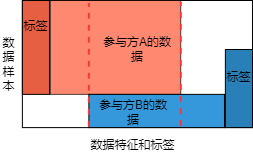
\includegraphics[width=0.3\textwidth]{chapters/imgs/FedClassA}}
	\hspace{0.01\textwidth}
	\subfigure[]{
		\label{FedClassB}
		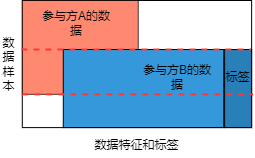
\includegraphics[width=0.3\textwidth]{chapters/imgs/FedClassB}}
	\hspace{0.01\textwidth}
	\subfigure[]{
		\label{FedClassC}
		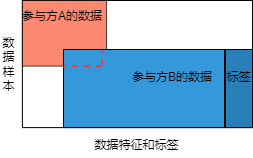
\includegraphics[width=0.3\textwidth]{chapters/imgs/FedClassC}}
	
	\bicaption[\xiaosi \songti 联邦学习分类]%
	{\centering \wuhao 联邦学习分类。(a) 横向联邦学习;(b) 纵向联邦学习;(c) 迁移联邦学习}%
	{\centering \wuhao Federated Learning Classification. (a) Horizontal Federated Learning; (b) Vertical Federated Learning; (c) Transfer Federated Learning}	
	\label{fig:FedClass}
\end{figure}

% \begin{figure} - 开始一个浮动图形环境
% 	[!htbp] - 这些是位置指定符,告诉LaTeX尝试将图形放置在哪里:
% 	! - 覆盖LaTeX的内部参数,用于确定"良好"的浮动位置
% 	h - Here(此处):尝试将图形放在文本中出现的确切位置
% 	t - Top(顶部):允许图形放置在页面顶部
% 	b - Bottom(底部):允许图形放置在页面底部
% 	p - Page of floats(浮动页):允许图形放置在仅包含浮动体的单独页面上
% 	这段代码不完整,因为它缺少图形内容和用于关闭环境的\end{figure}命令。


\begin{figure}[!htbp]
	\centering
	\vspace{0.5cm} % 调整图片与上文的间距
	\captionsetup{size=footnotesize}
	
	\subfigure[]{\label{RQ2.1.sub1}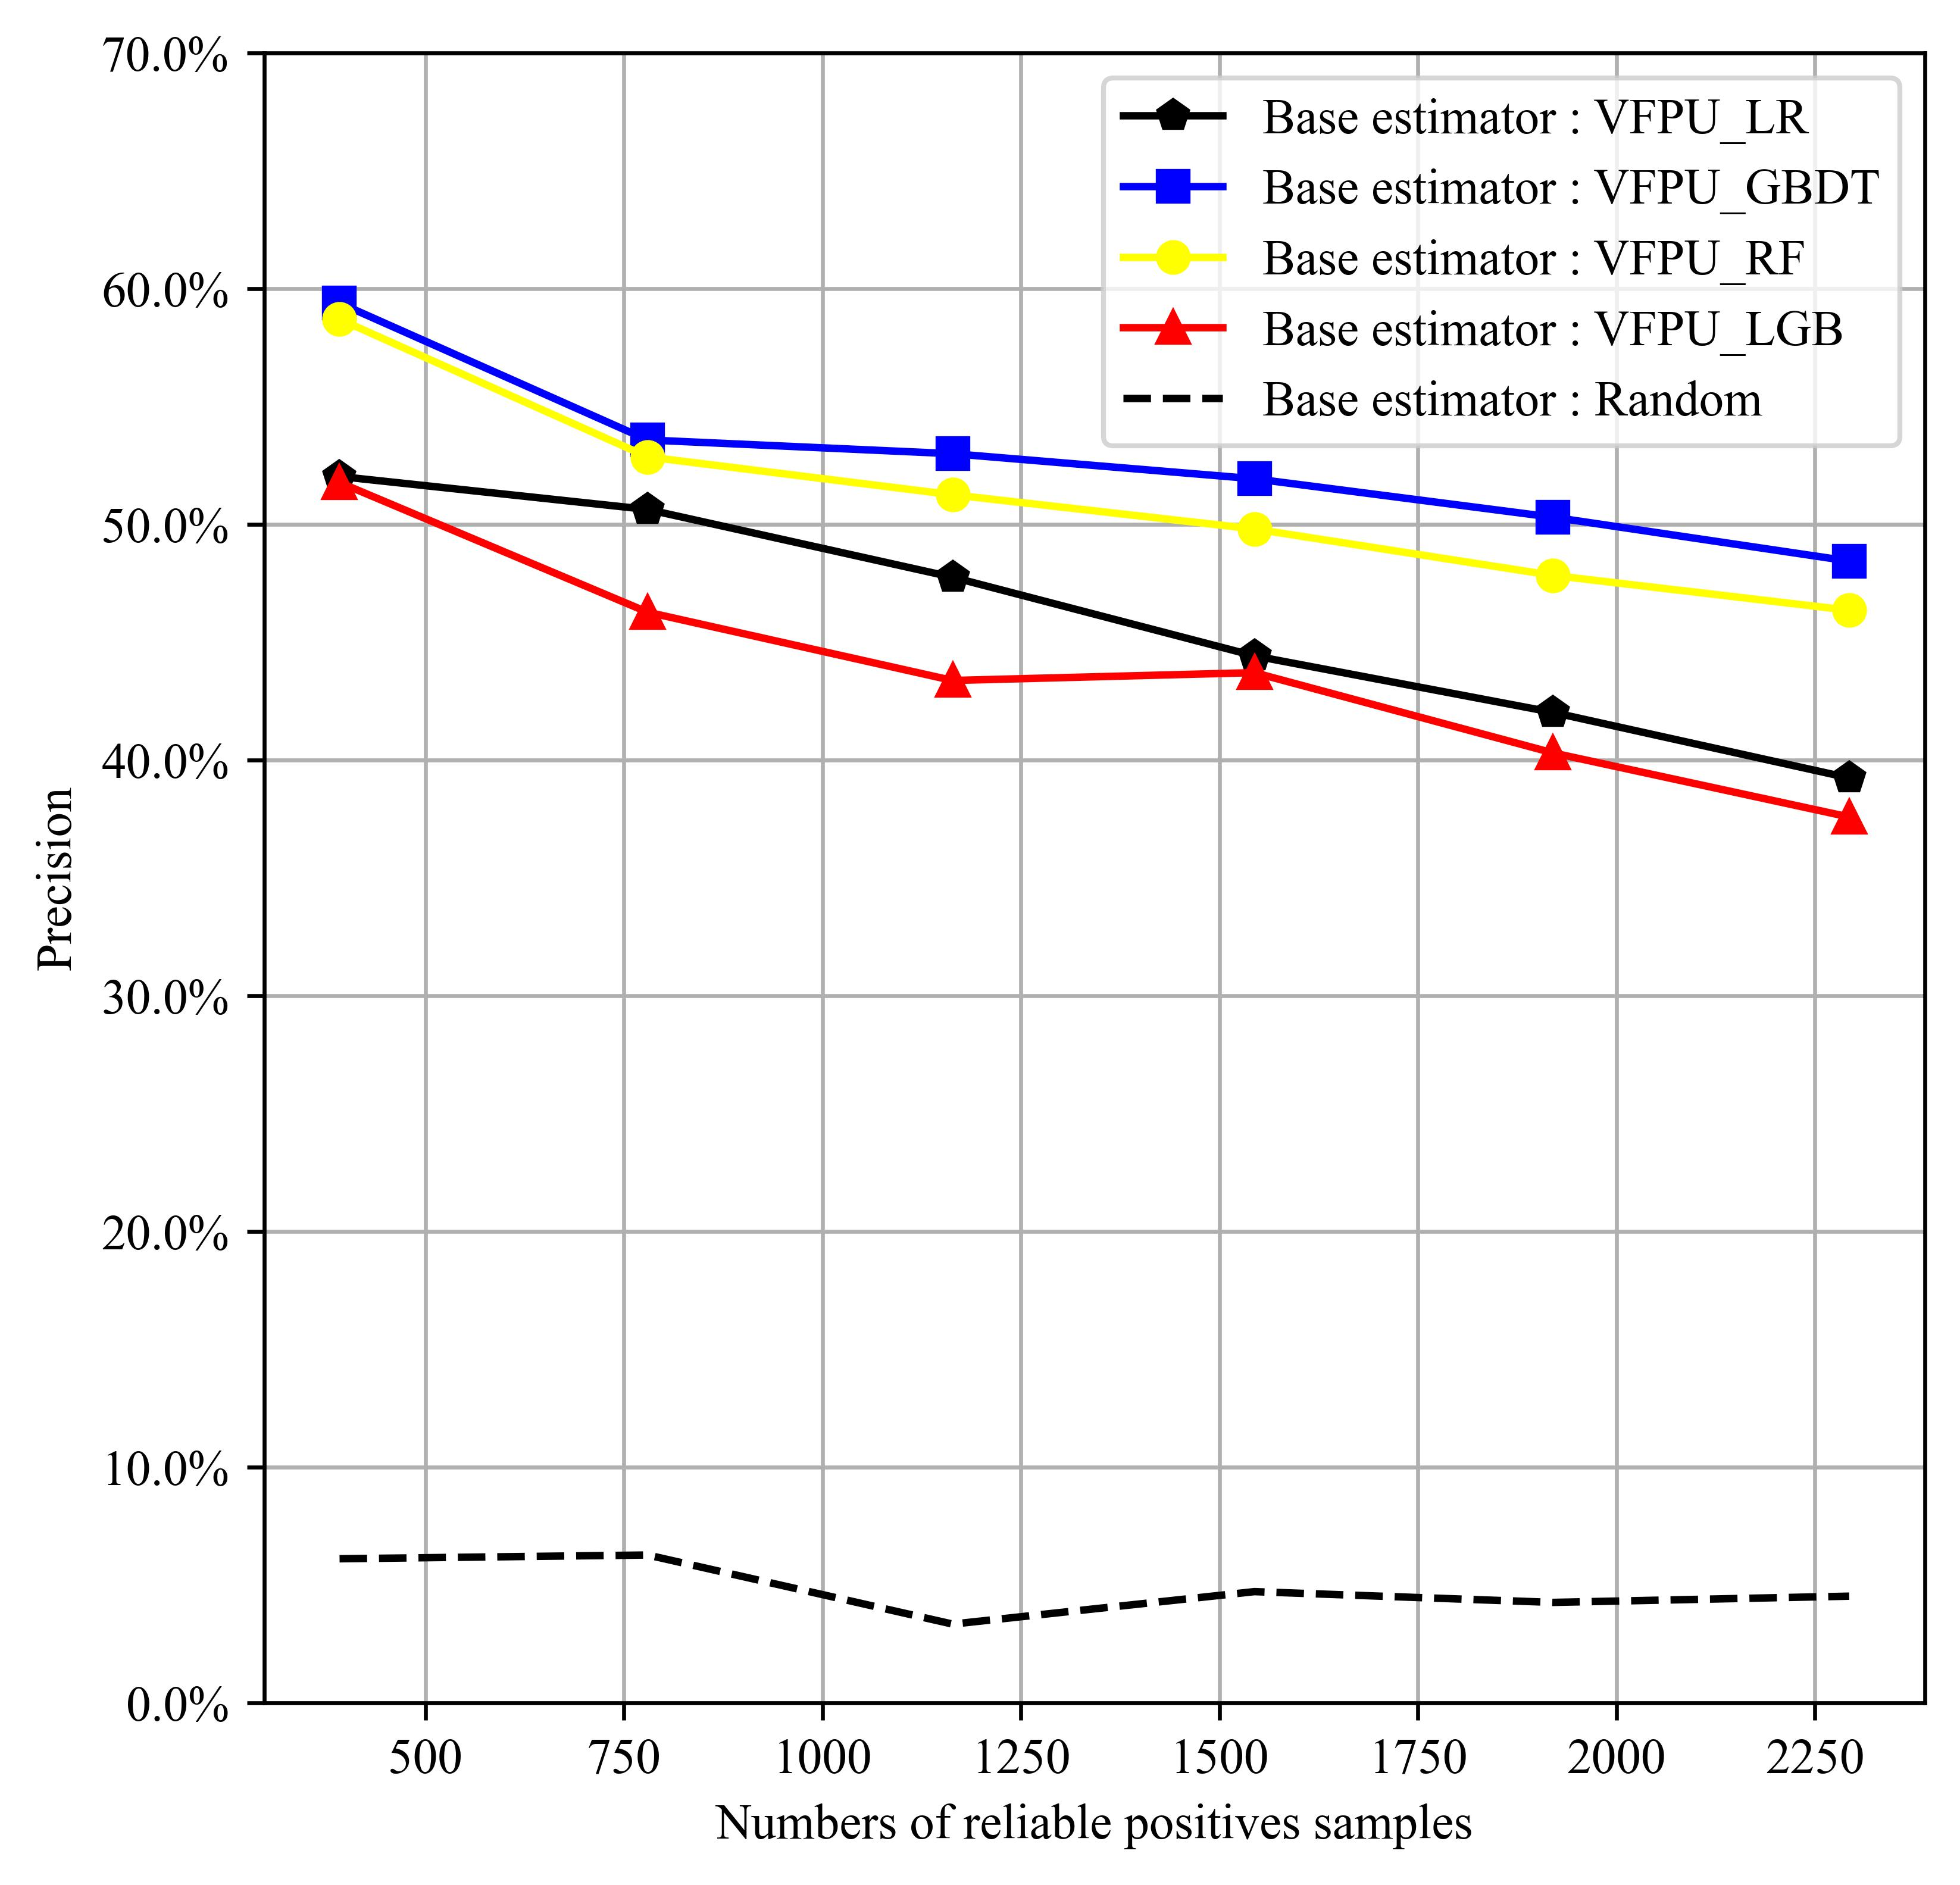
\includegraphics[width=0.45\textwidth,height=5.1cm]{chapters/imgs/Figure 2 (1) in JEPG format}}
	\subfigure[]{\label{RQ2.1.sub2}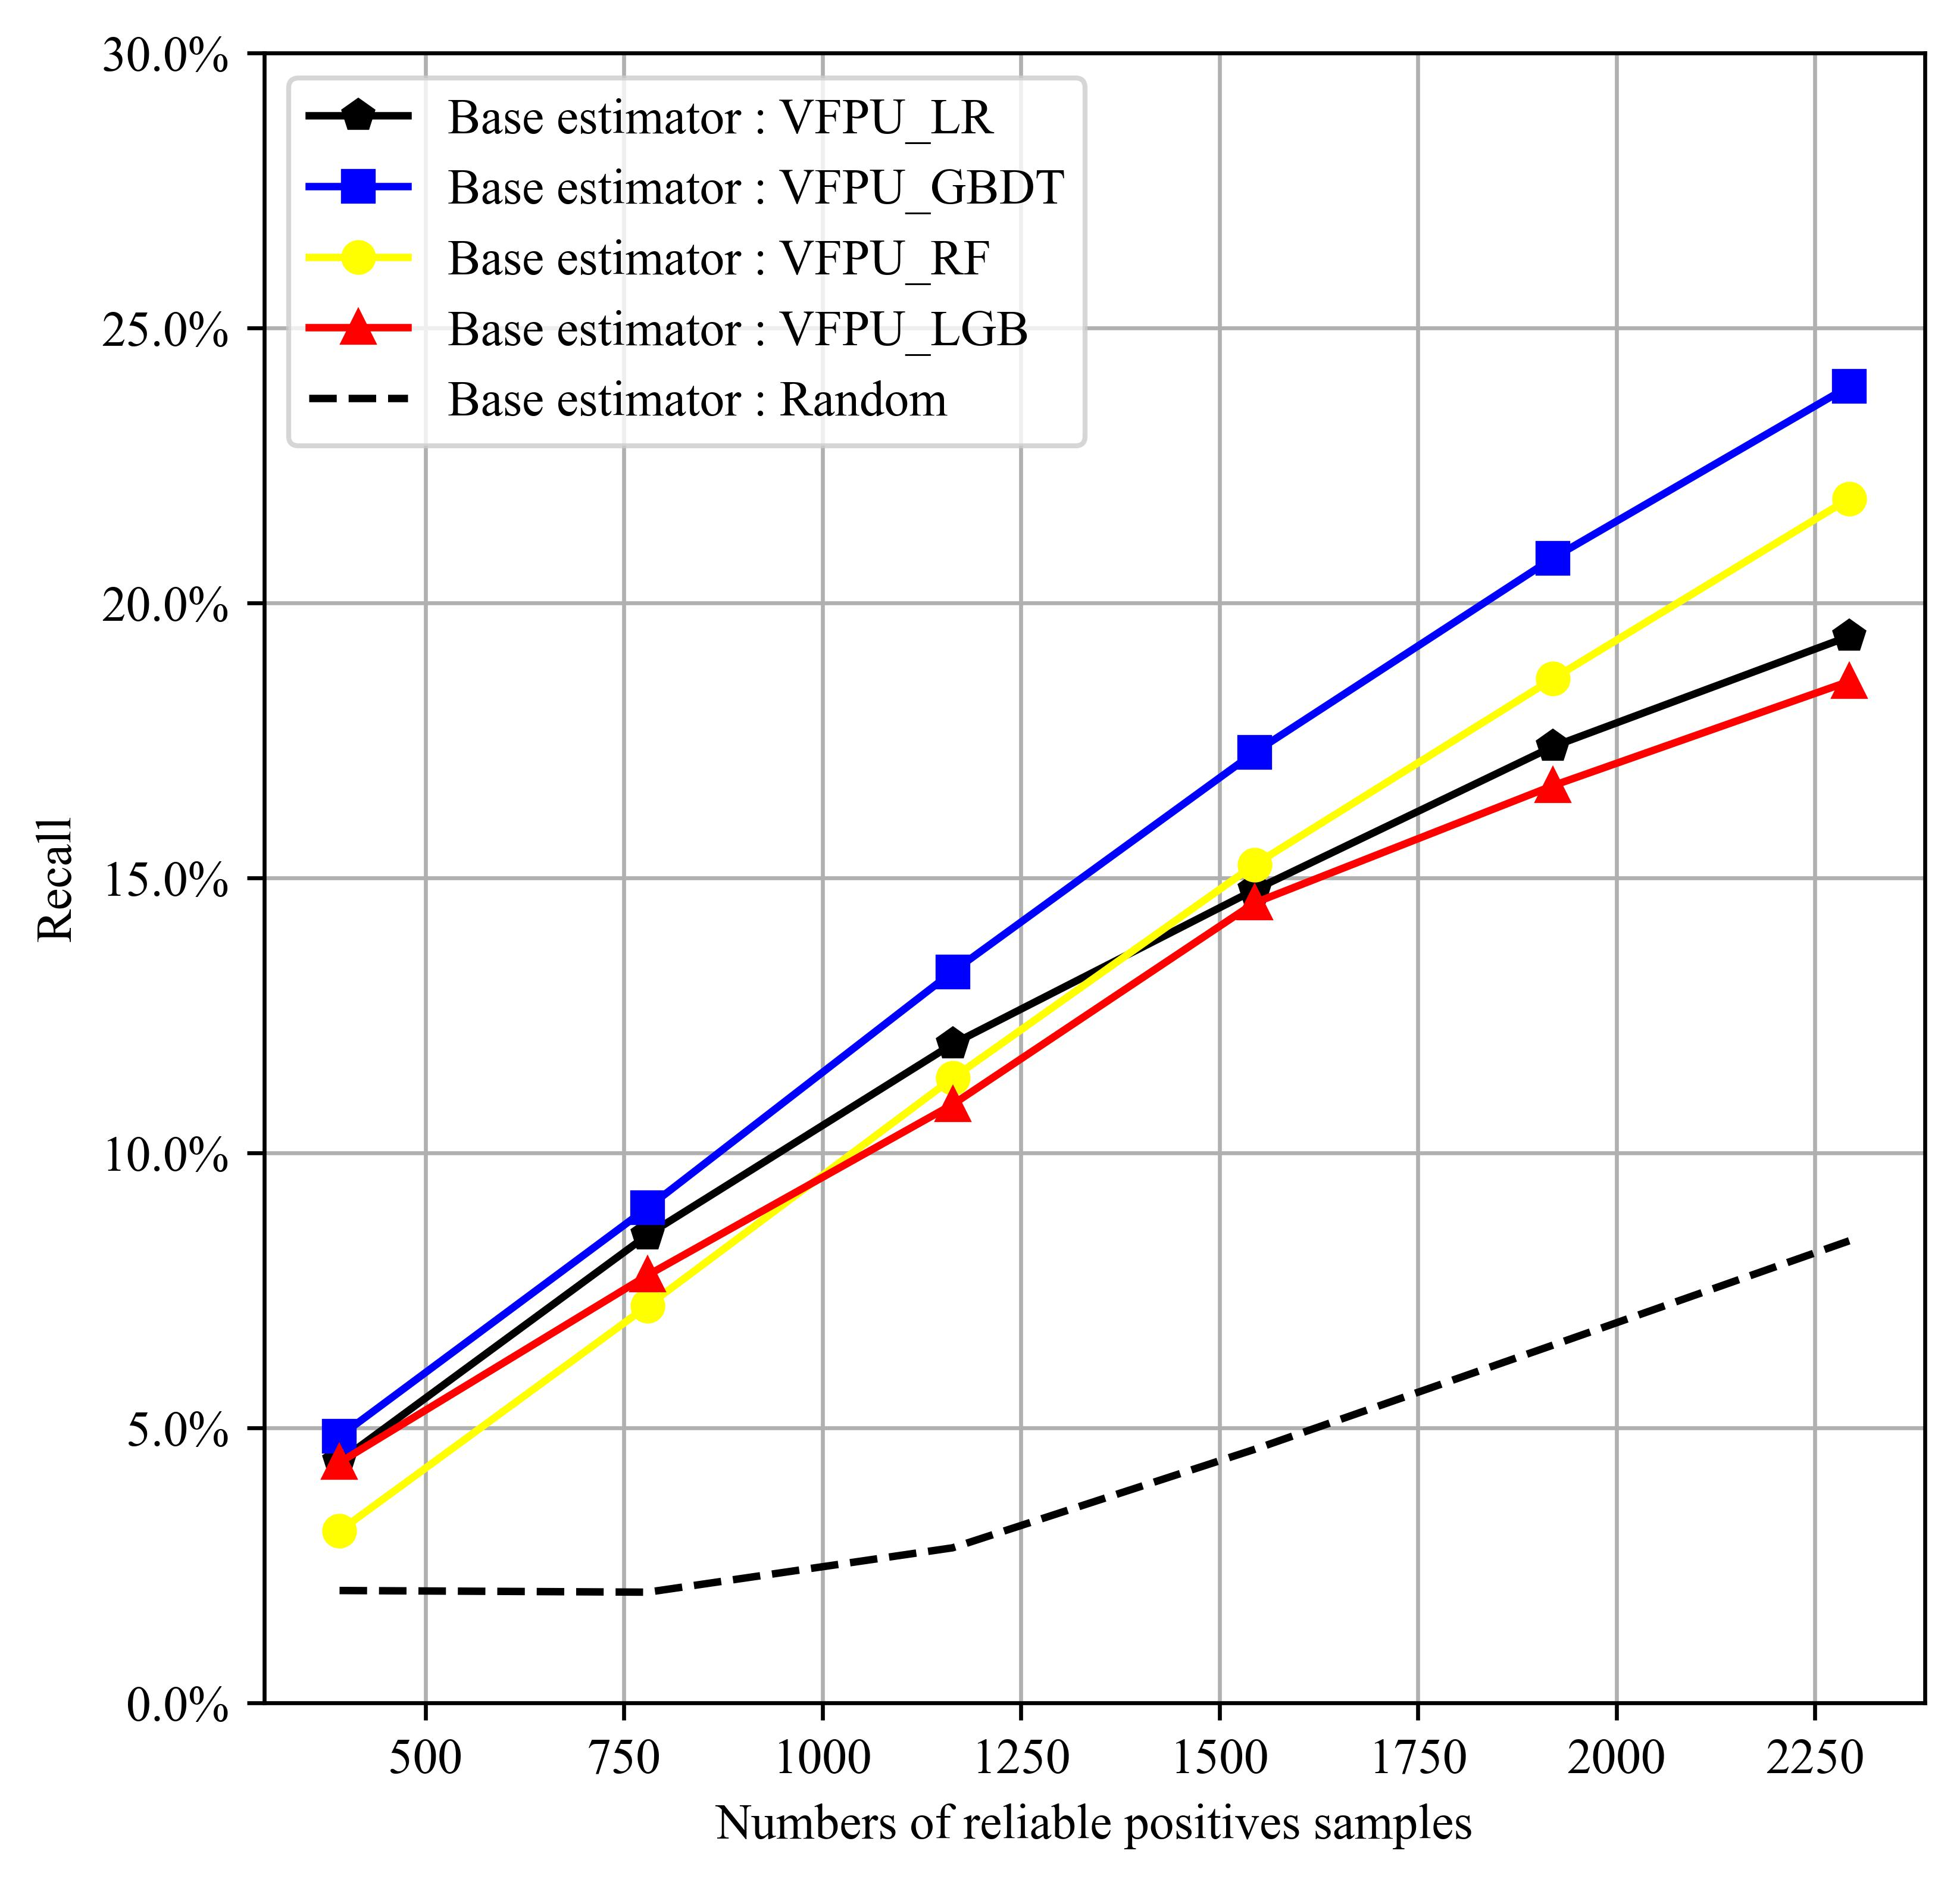
\includegraphics[width=0.45\textwidth,height=5.1cm]{chapters/imgs/Figure 2 (2) in JEPG format}}
	\subfigure[]{\label{RQ2.1.sub3}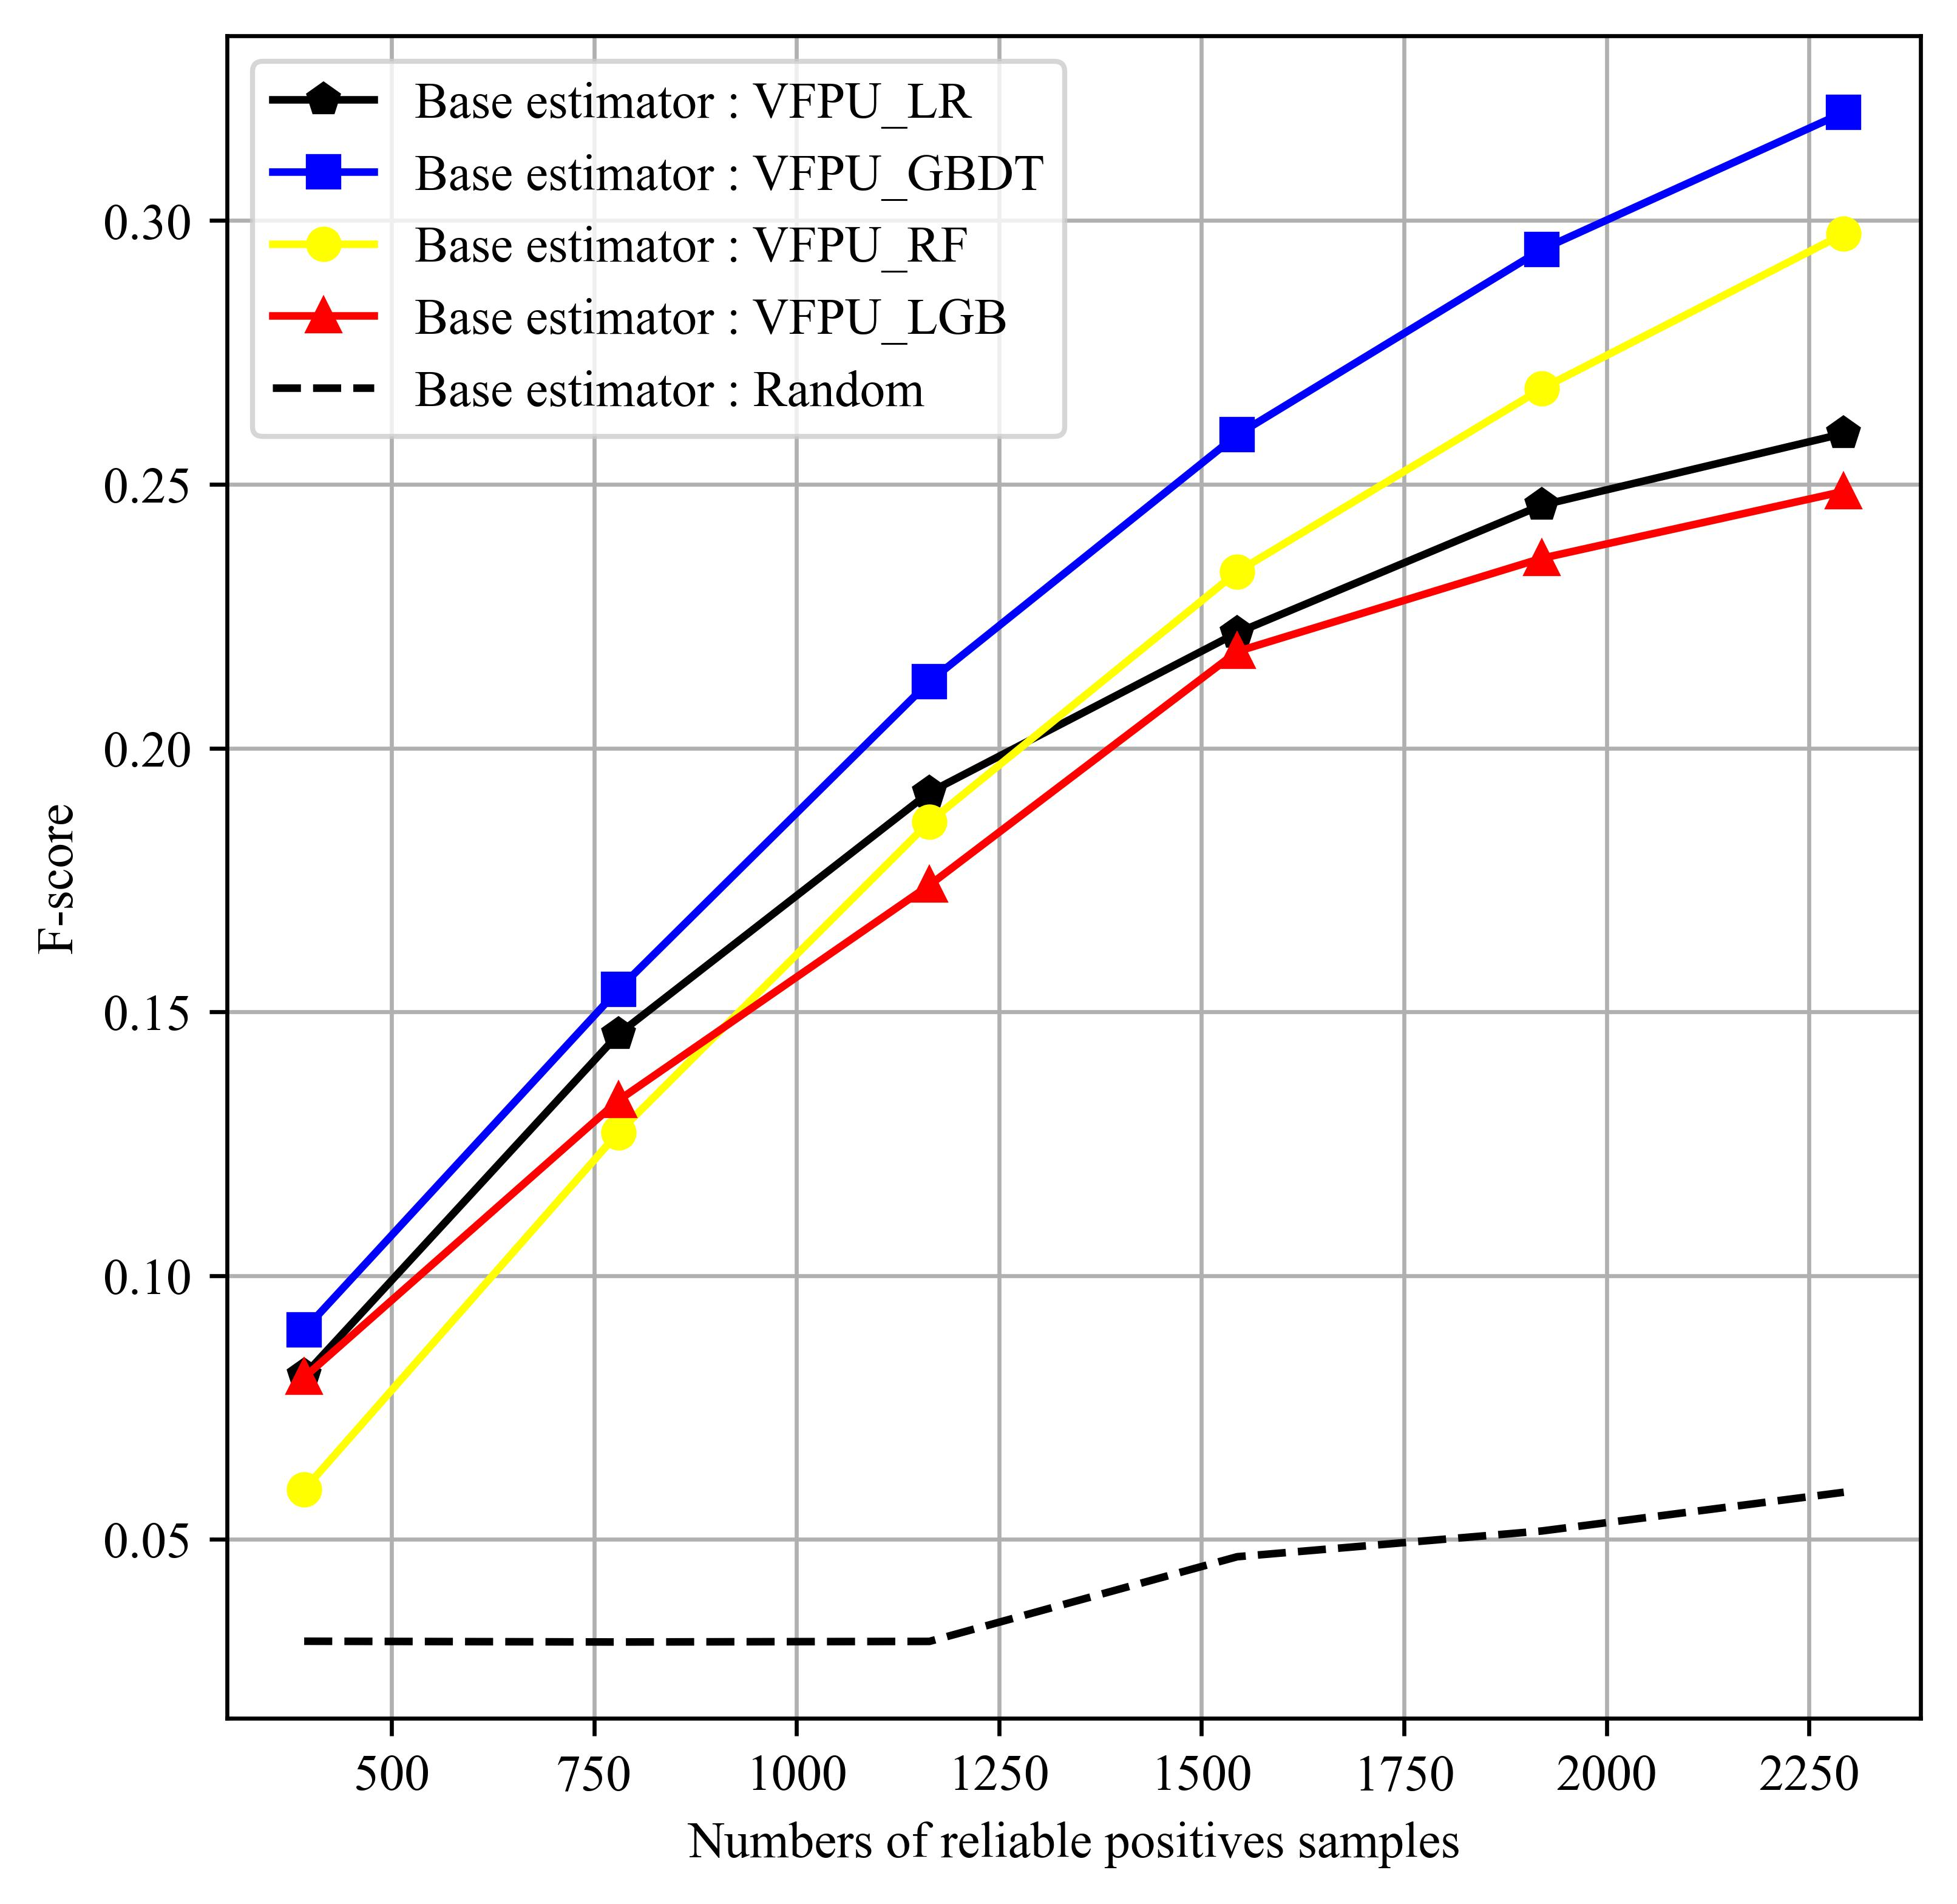
\includegraphics[width=0.45\textwidth,height=5.1cm]{chapters/imgs/Figure 2 (3) in JEPG format}}
	\subfigure[]{\label{RQ2.1.sub4}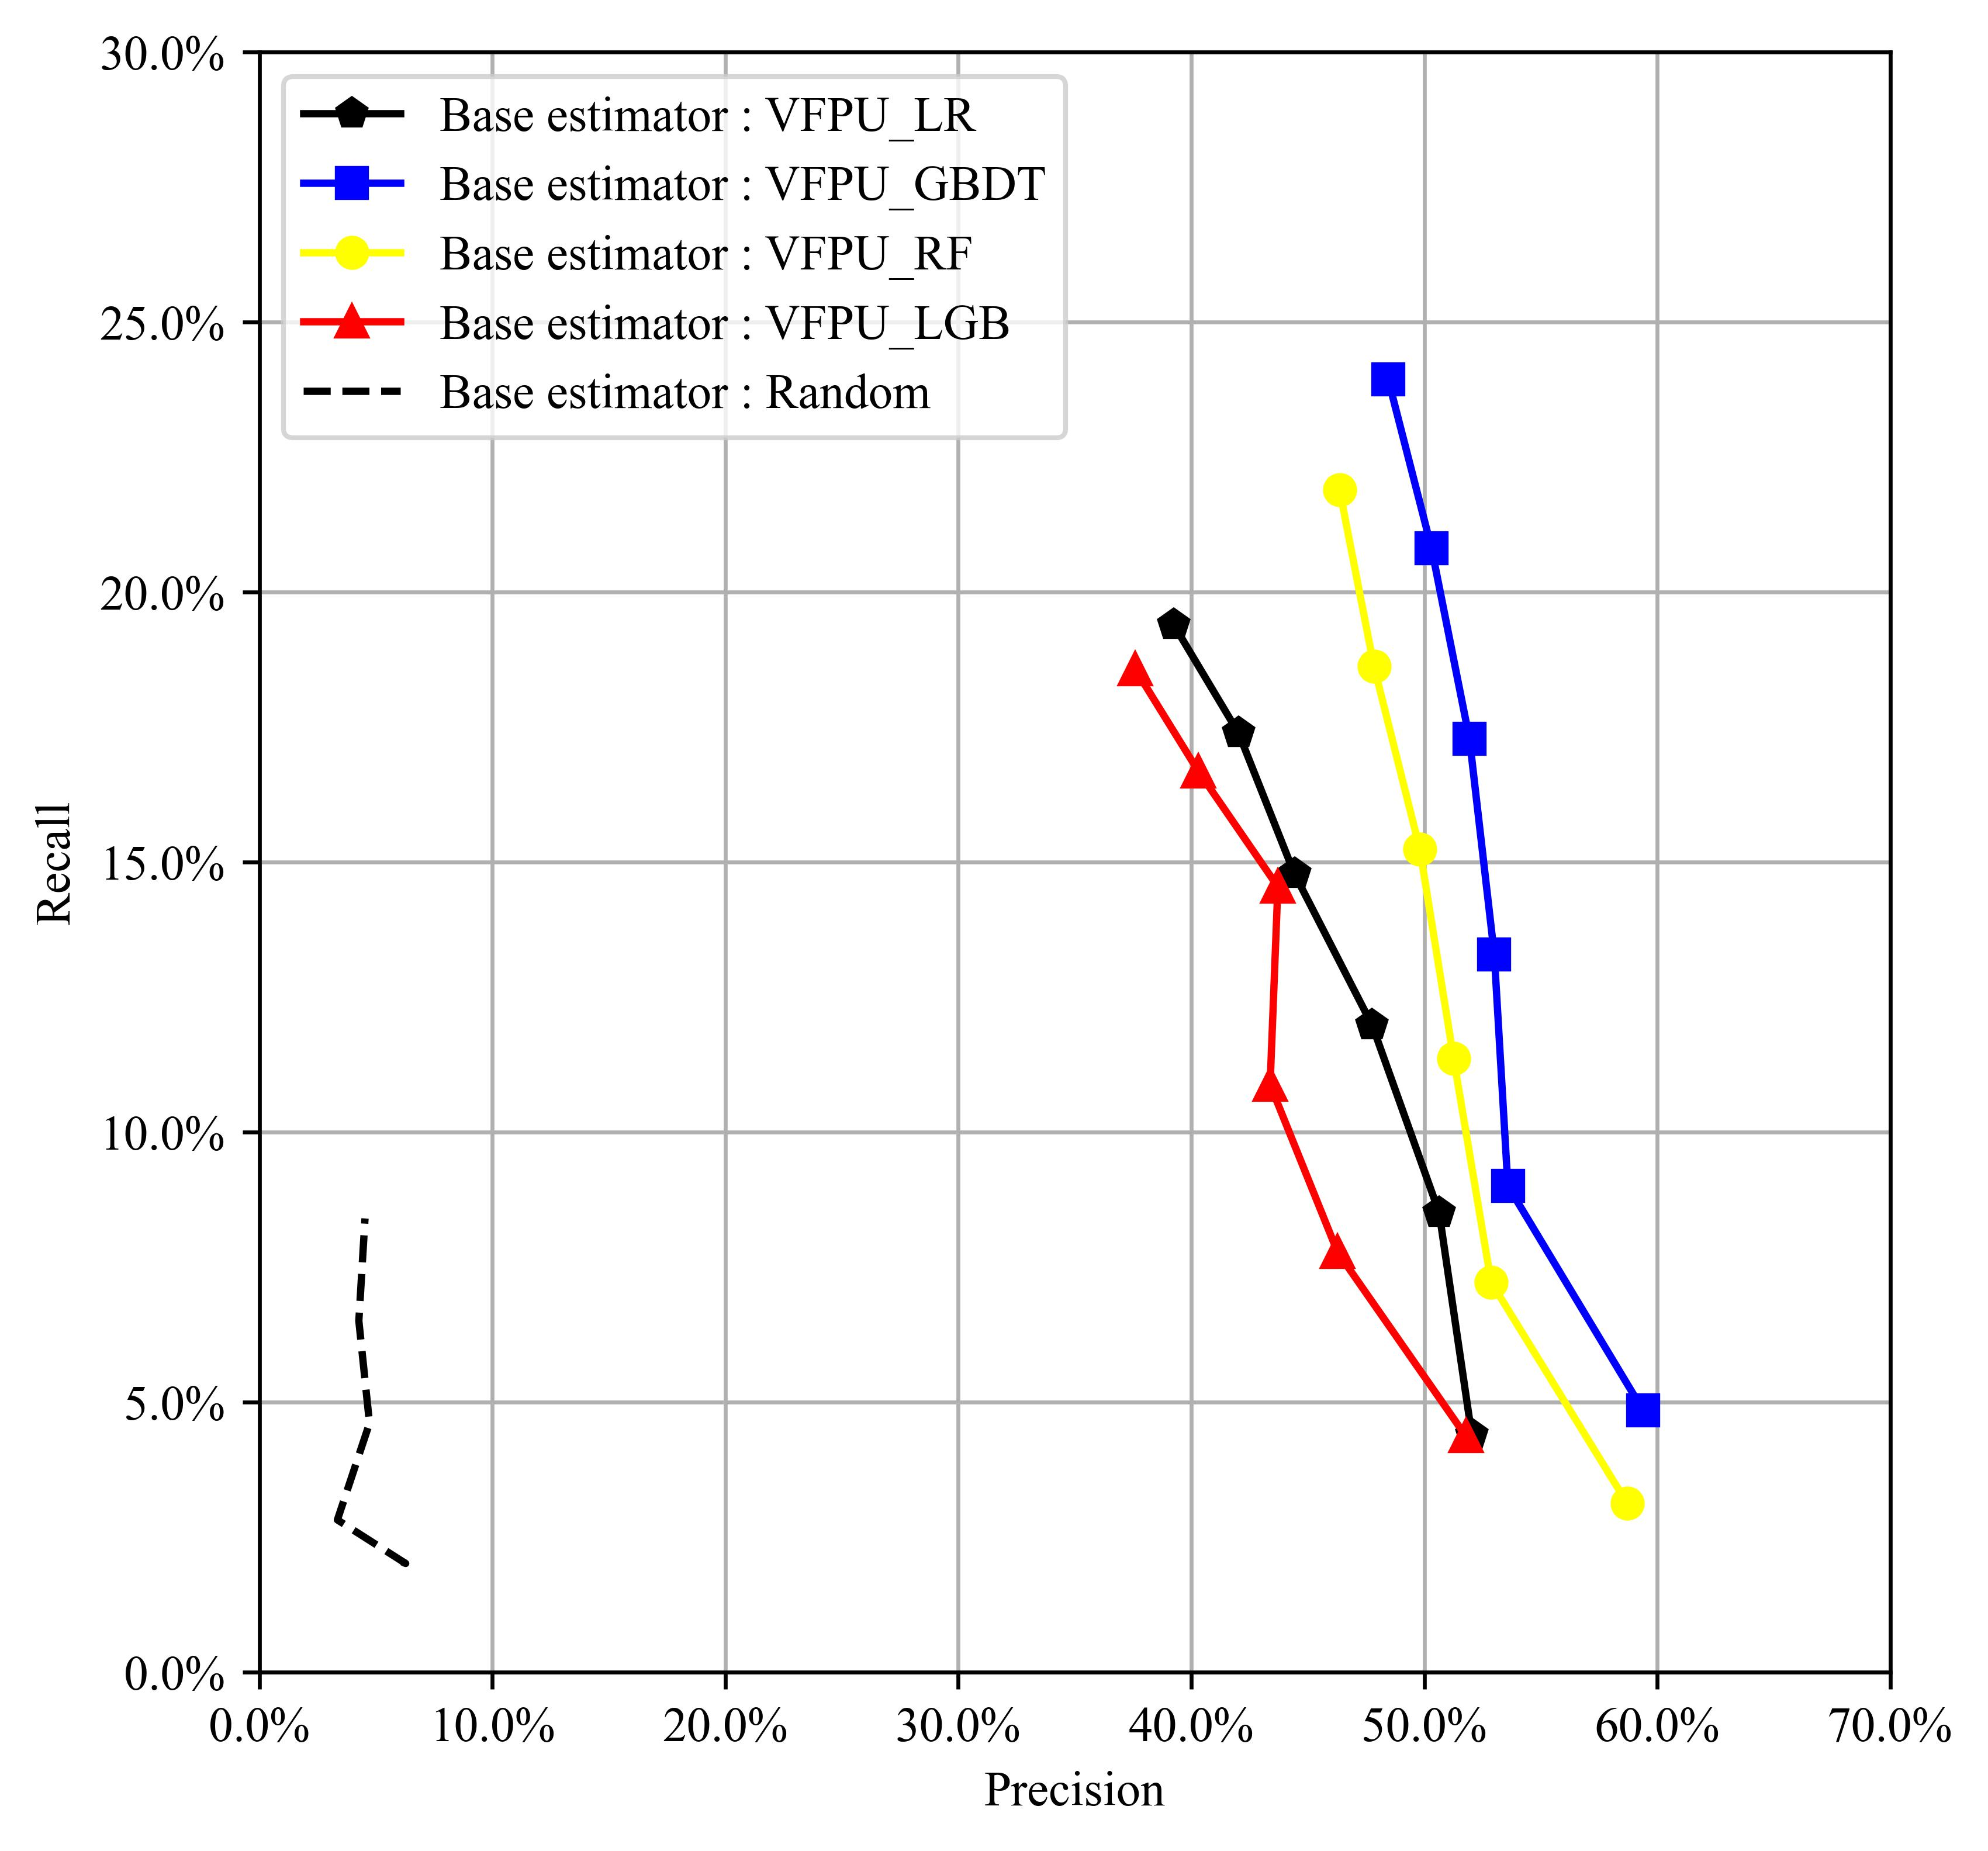
\includegraphics[width=0.45\textwidth,height=5.1cm]{chapters/imgs/Figure 2 (4) in JEPG format}}
	\begin{itemize}[leftmargin=1.6cm,rightmargin=1.6cm]
		\item[\quad] \bicaption[\xiaosi 不同基学器在不同可靠正样本数量下的性能]
	{\centering \wuhao 不同基学器在不同可靠正样本数量下的性能:(a)精度;(b)召回率;(c)F-score;(d)精度-召回率(Bank 数据集)}
	{\centering \wuhao Performance of Different Base Estimators with Varying Reliable Positive Samples: (a) Precision; (b) Recall; (c) F-score; (d) Precision-Recall (The Bank Marketing Dataset)}
	\end{itemize}
	\label{RQ2.1}
\end{figure}






\begin{figure}[!htbp]
	\centering
%	\setlength{\subfigcapskip}{0.1cm}
	
	\captionsetup{size=footnotesize}
	\begin{subfigure}{0.45\textwidth}
		\centering
		\captionsetup{skip=1pt}
		\captionsetup{size=scriptsize}
		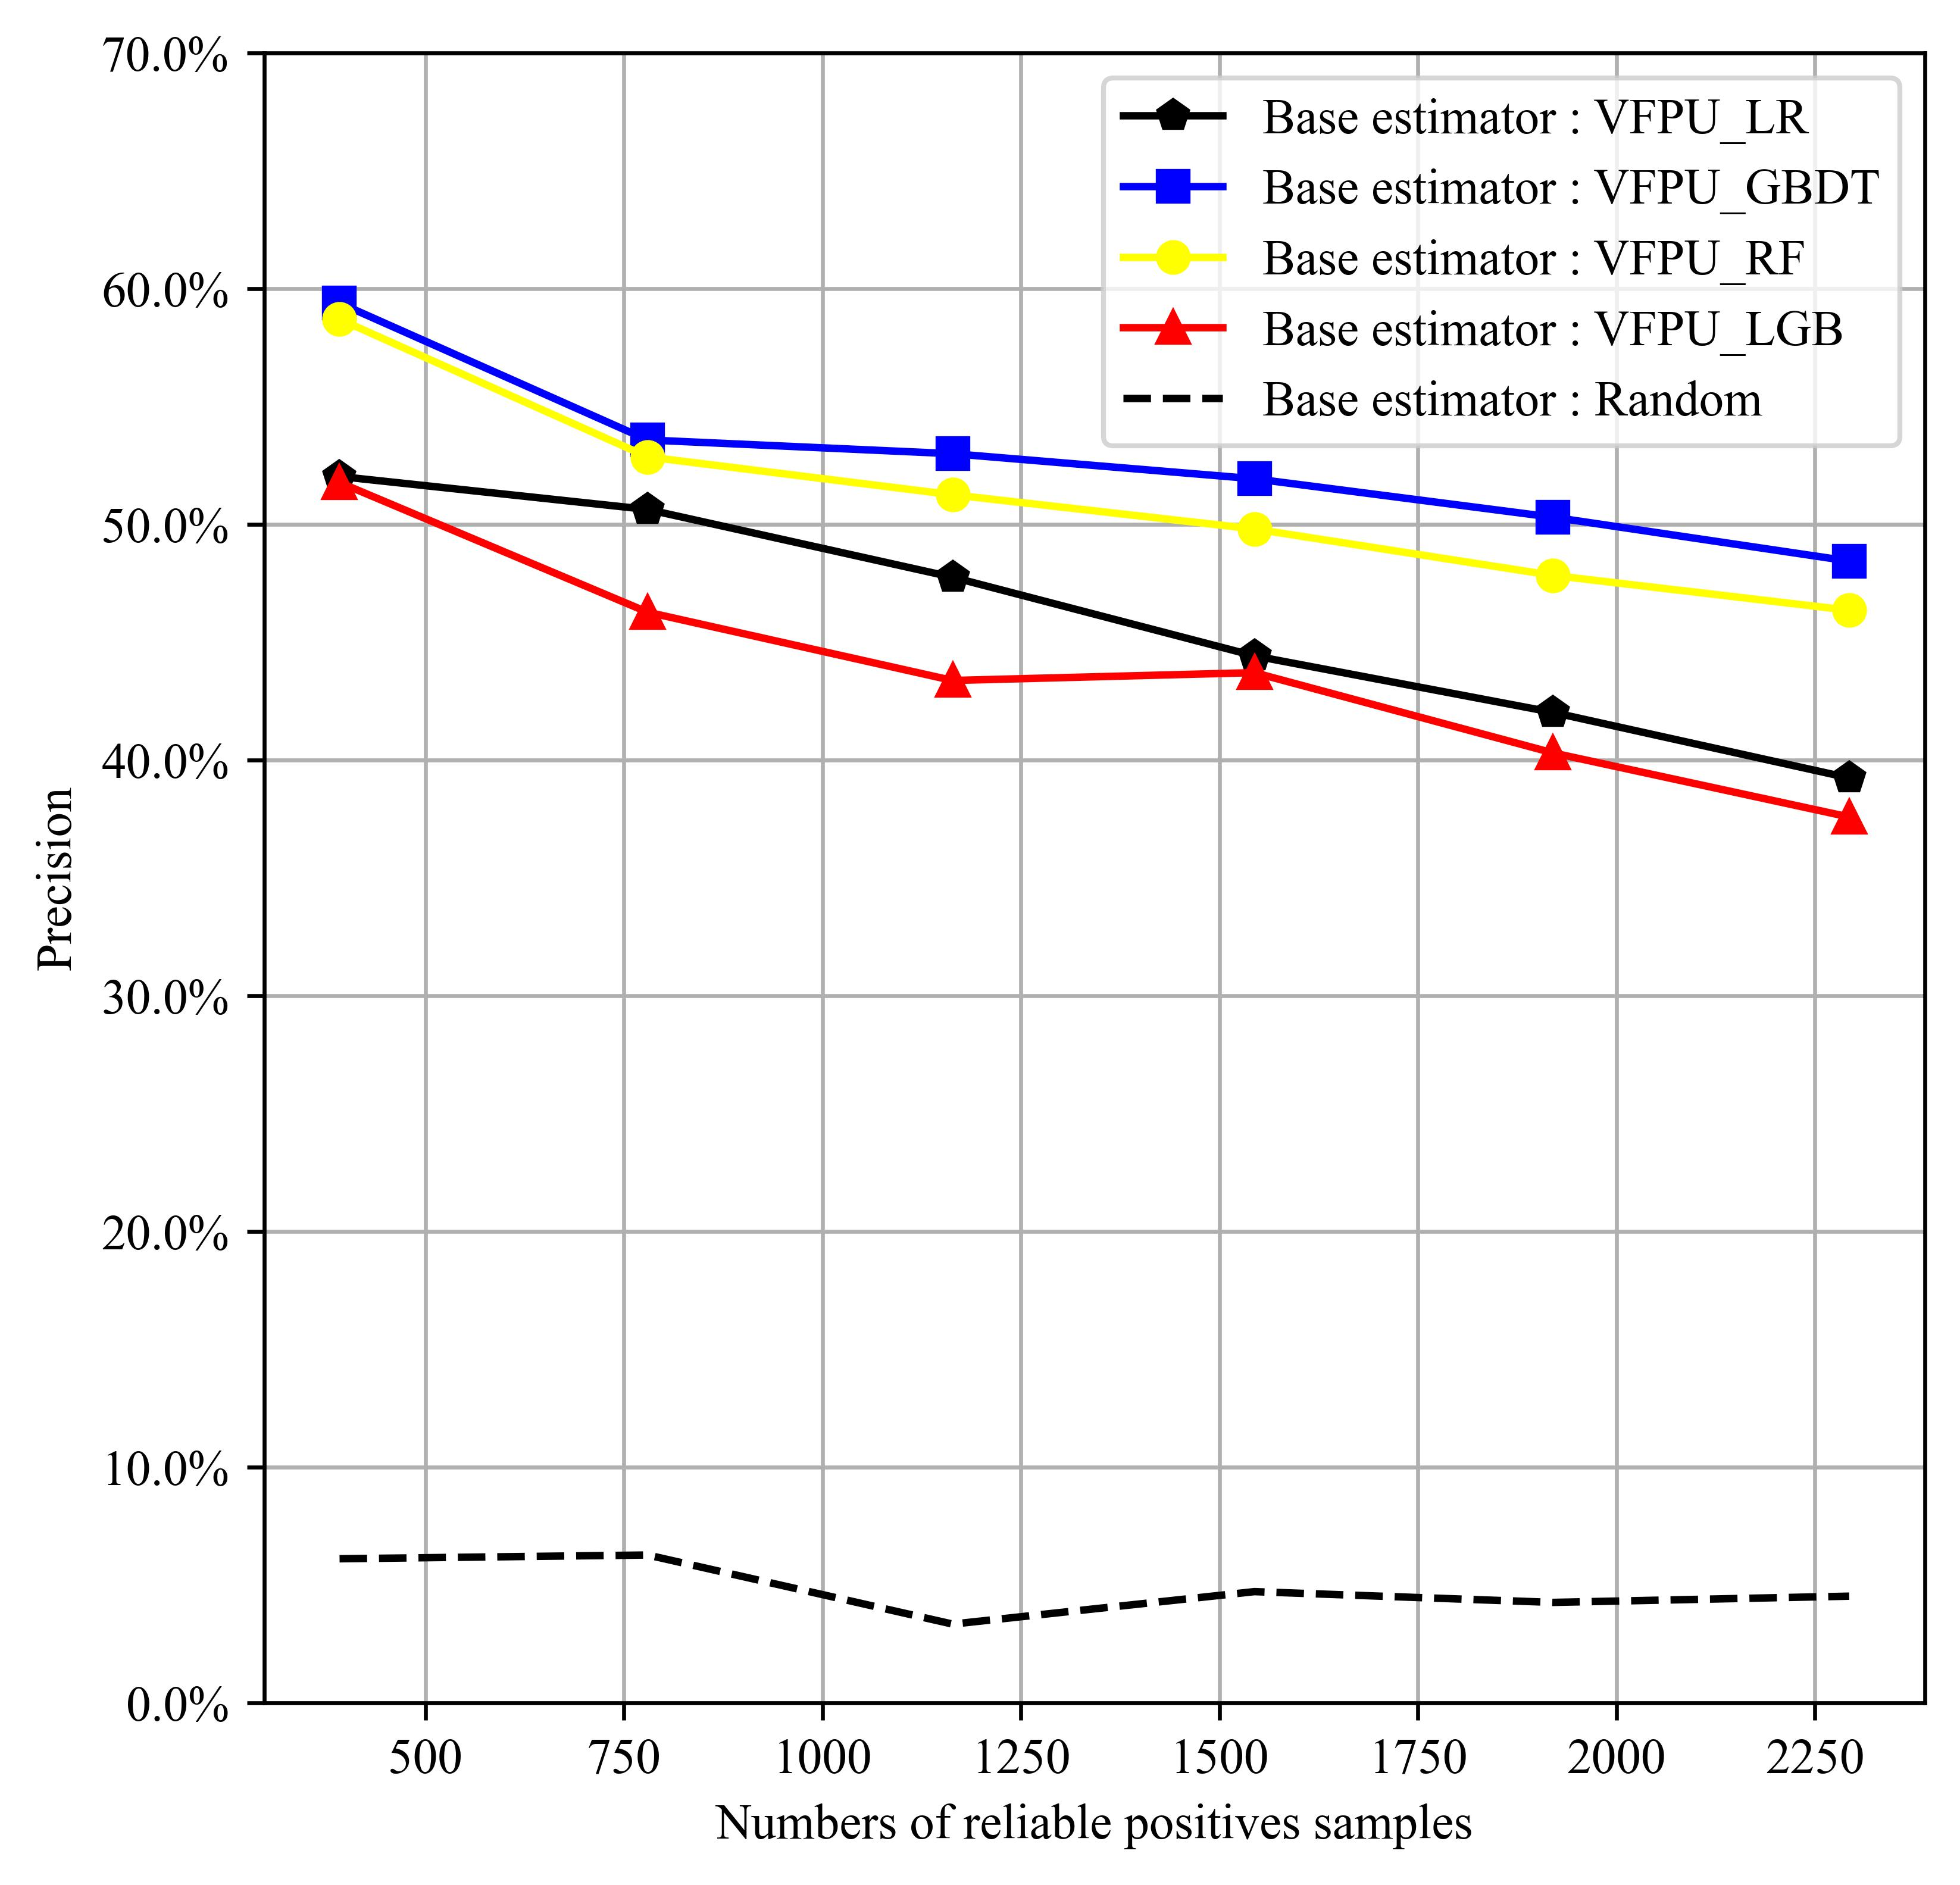
\includegraphics[width=0.9\textwidth,height=5.1cm]{chapters/imgs/Figure 2 (1) in JEPG format}
		\caption{Precision}
%		\vspace{0cm}
		\label{RQ2.1.sub1}
	\end{subfigure}
%	\hfill
%    \hspace{-1cm}
	\begin{subfigure}{0.45\textwidth}
		\centering
		\captionsetup{skip=4pt}
		\captionsetup{size=scriptsize}
		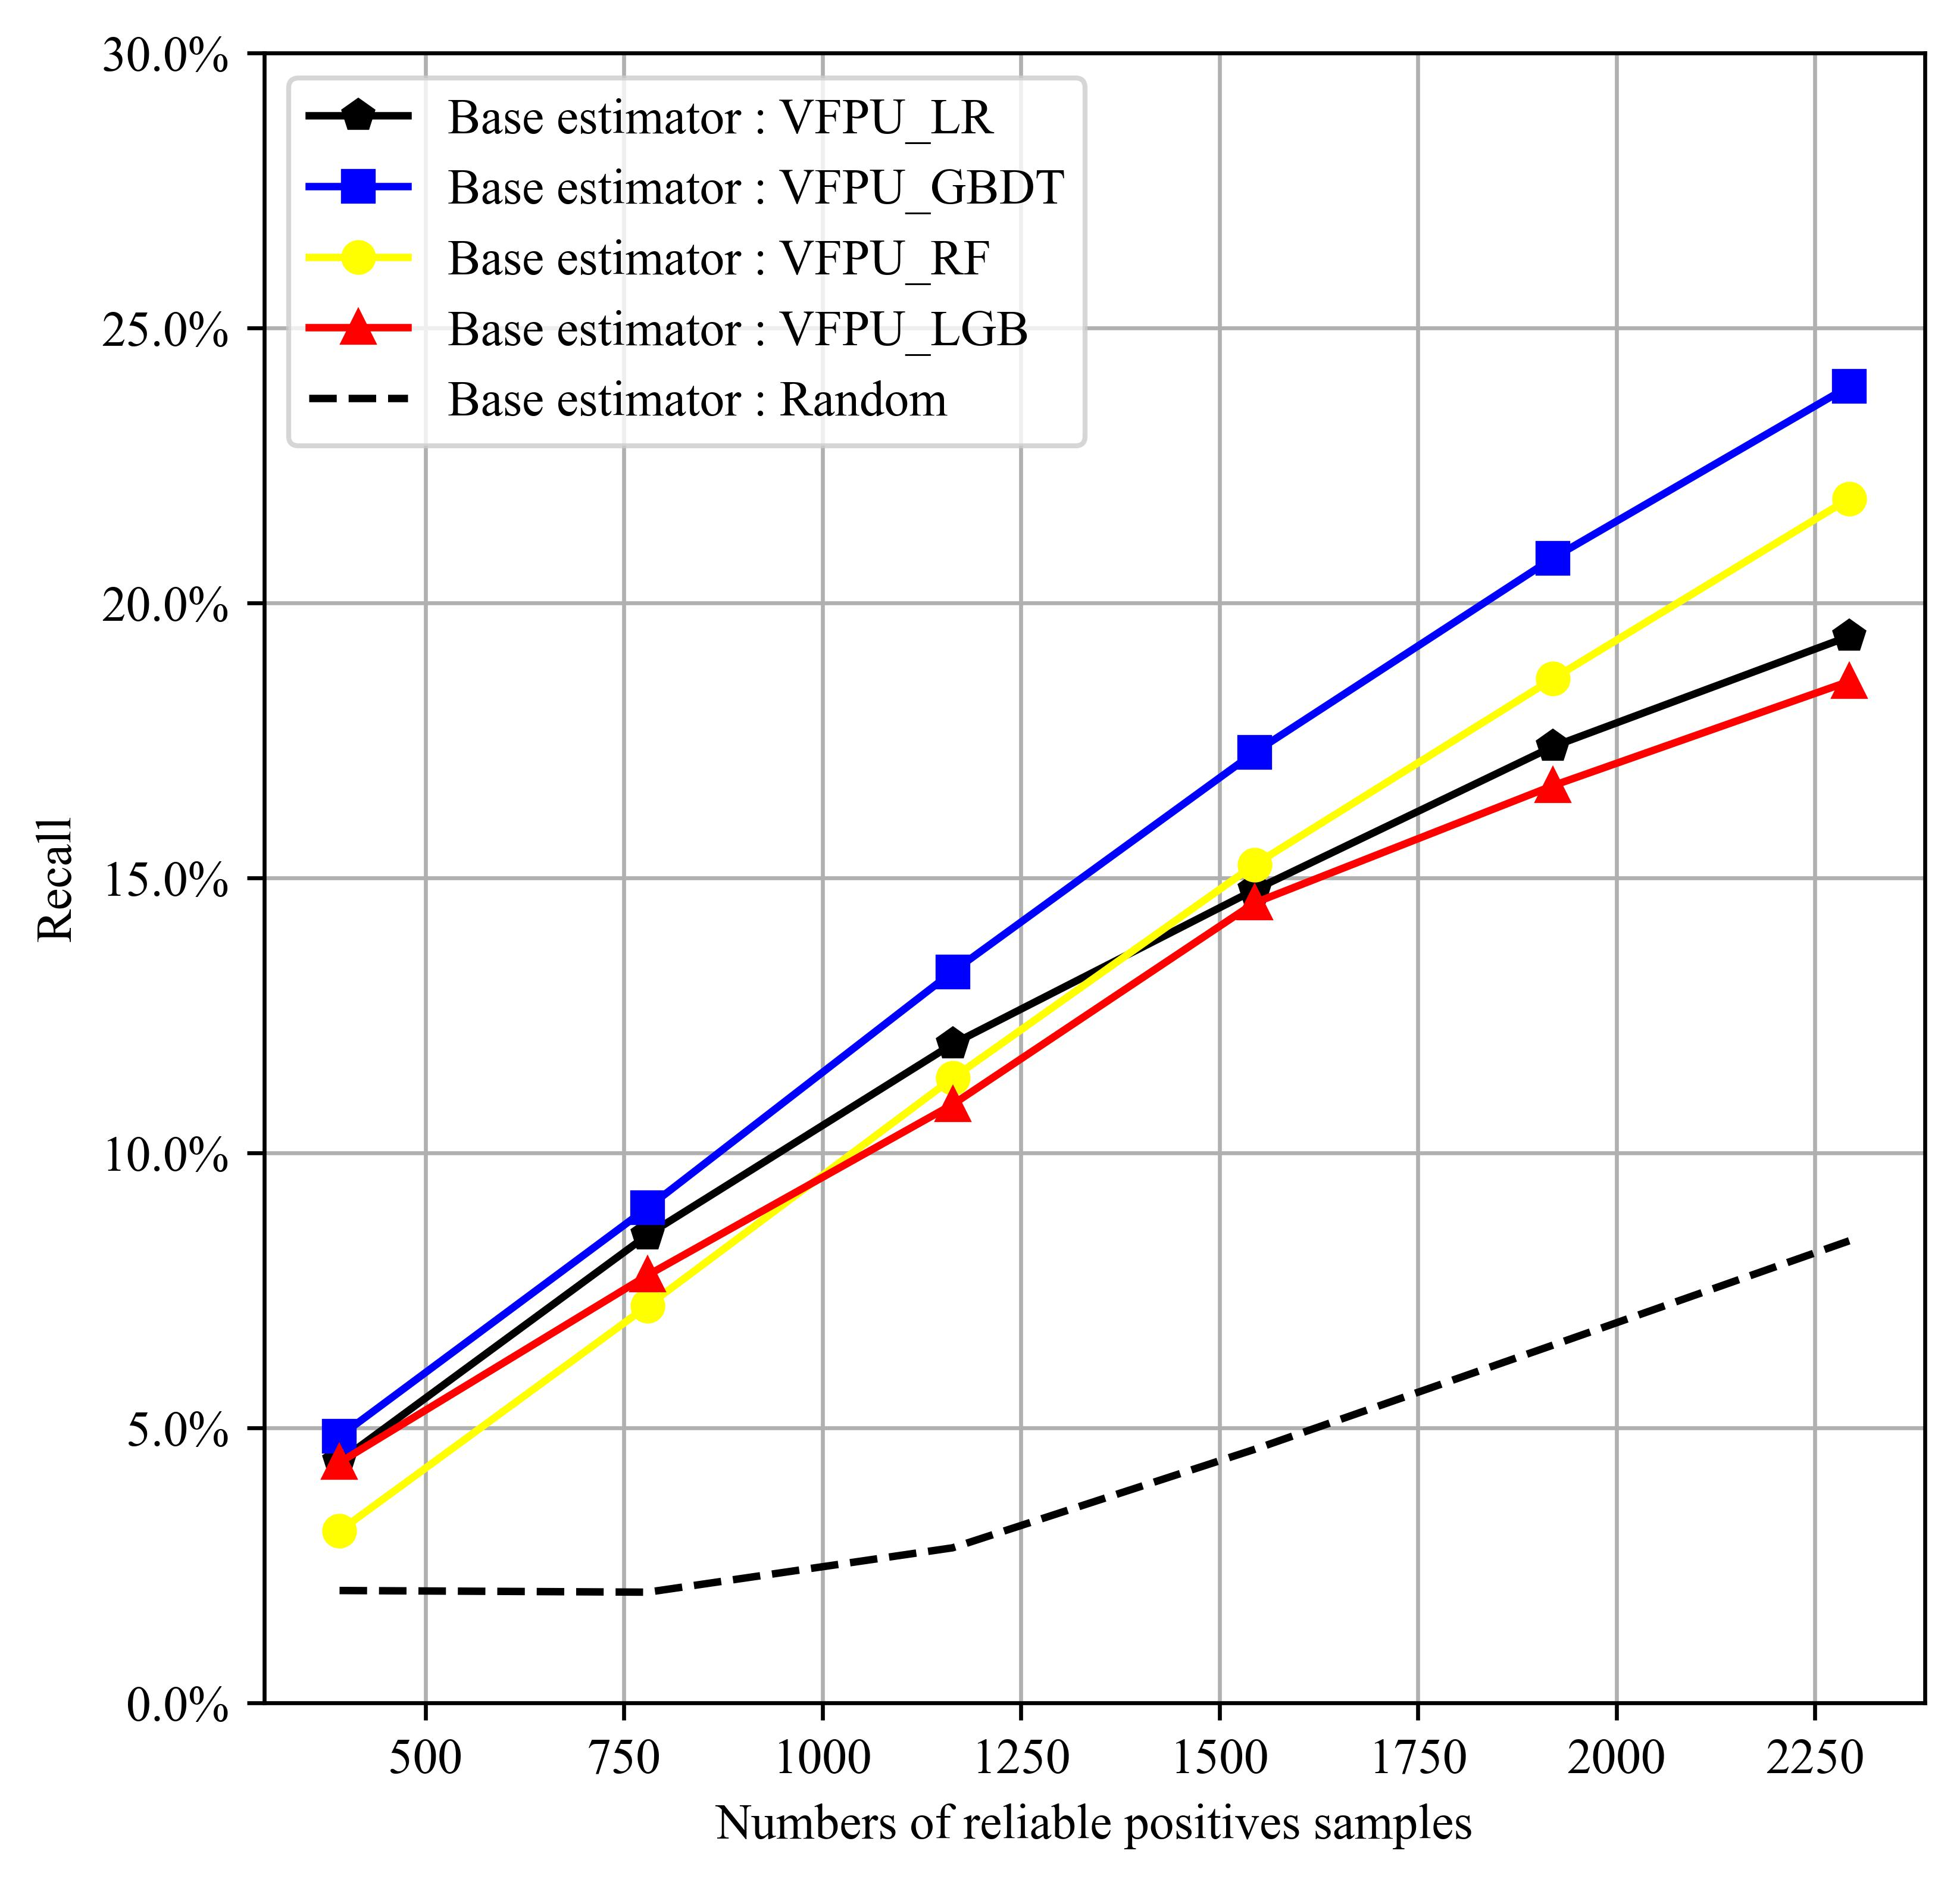
\includegraphics[width=0.9\textwidth,height=5.1cm]{chapters/imgs/Figure 2 (2) in JEPG format}
		\caption{Recall}
		\label{RQ2.1.sub2}
	\end{subfigure}
	
%	\vspace{0.05cm}
	
	\begin{subfigure}{0.45\textwidth}
		\centering
		\captionsetup{skip=4pt}
		\captionsetup{size=scriptsize}
		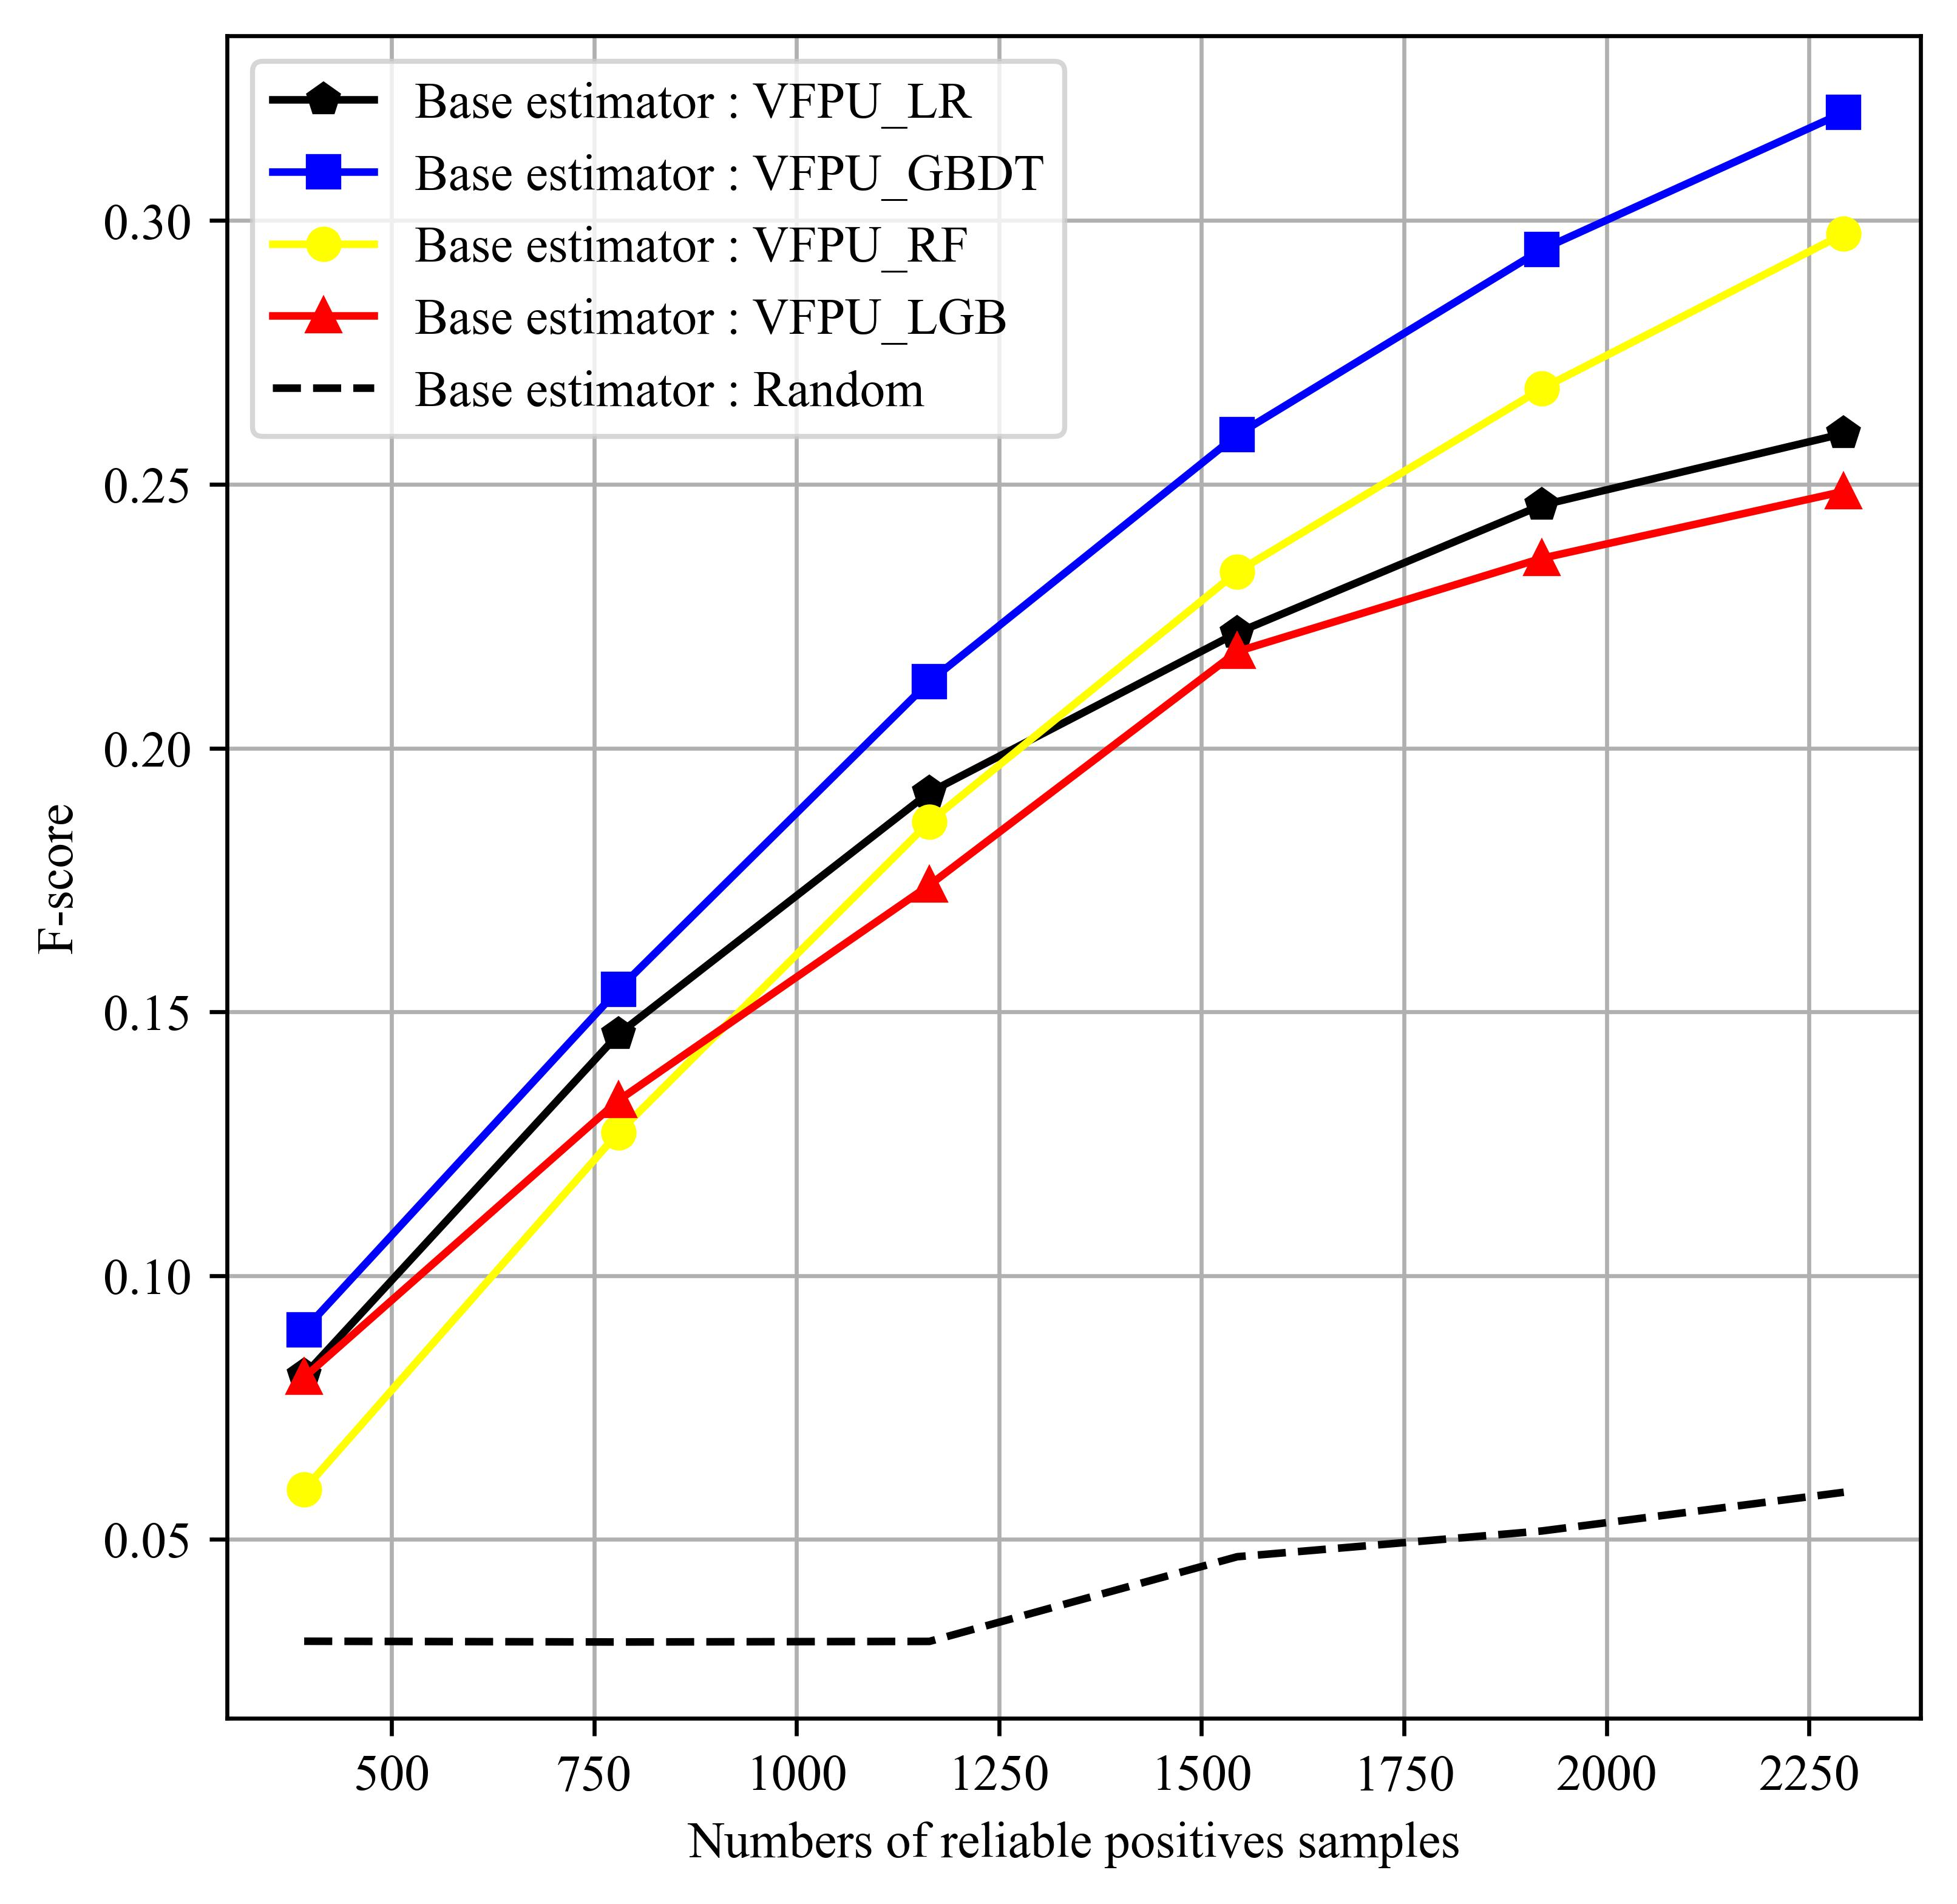
\includegraphics[width=0.9\textwidth,height=5.1cm]{chapters/imgs/Figure 2 (3) in JEPG format}
		\caption{F-score}
		\label{RQ2.1.sub3}
	\end{subfigure}
%\hfill
	\begin{subfigure}{0.45\textwidth}
		\centering
		\captionsetup{skip=4pt}
		\captionsetup{size=scriptsize}
		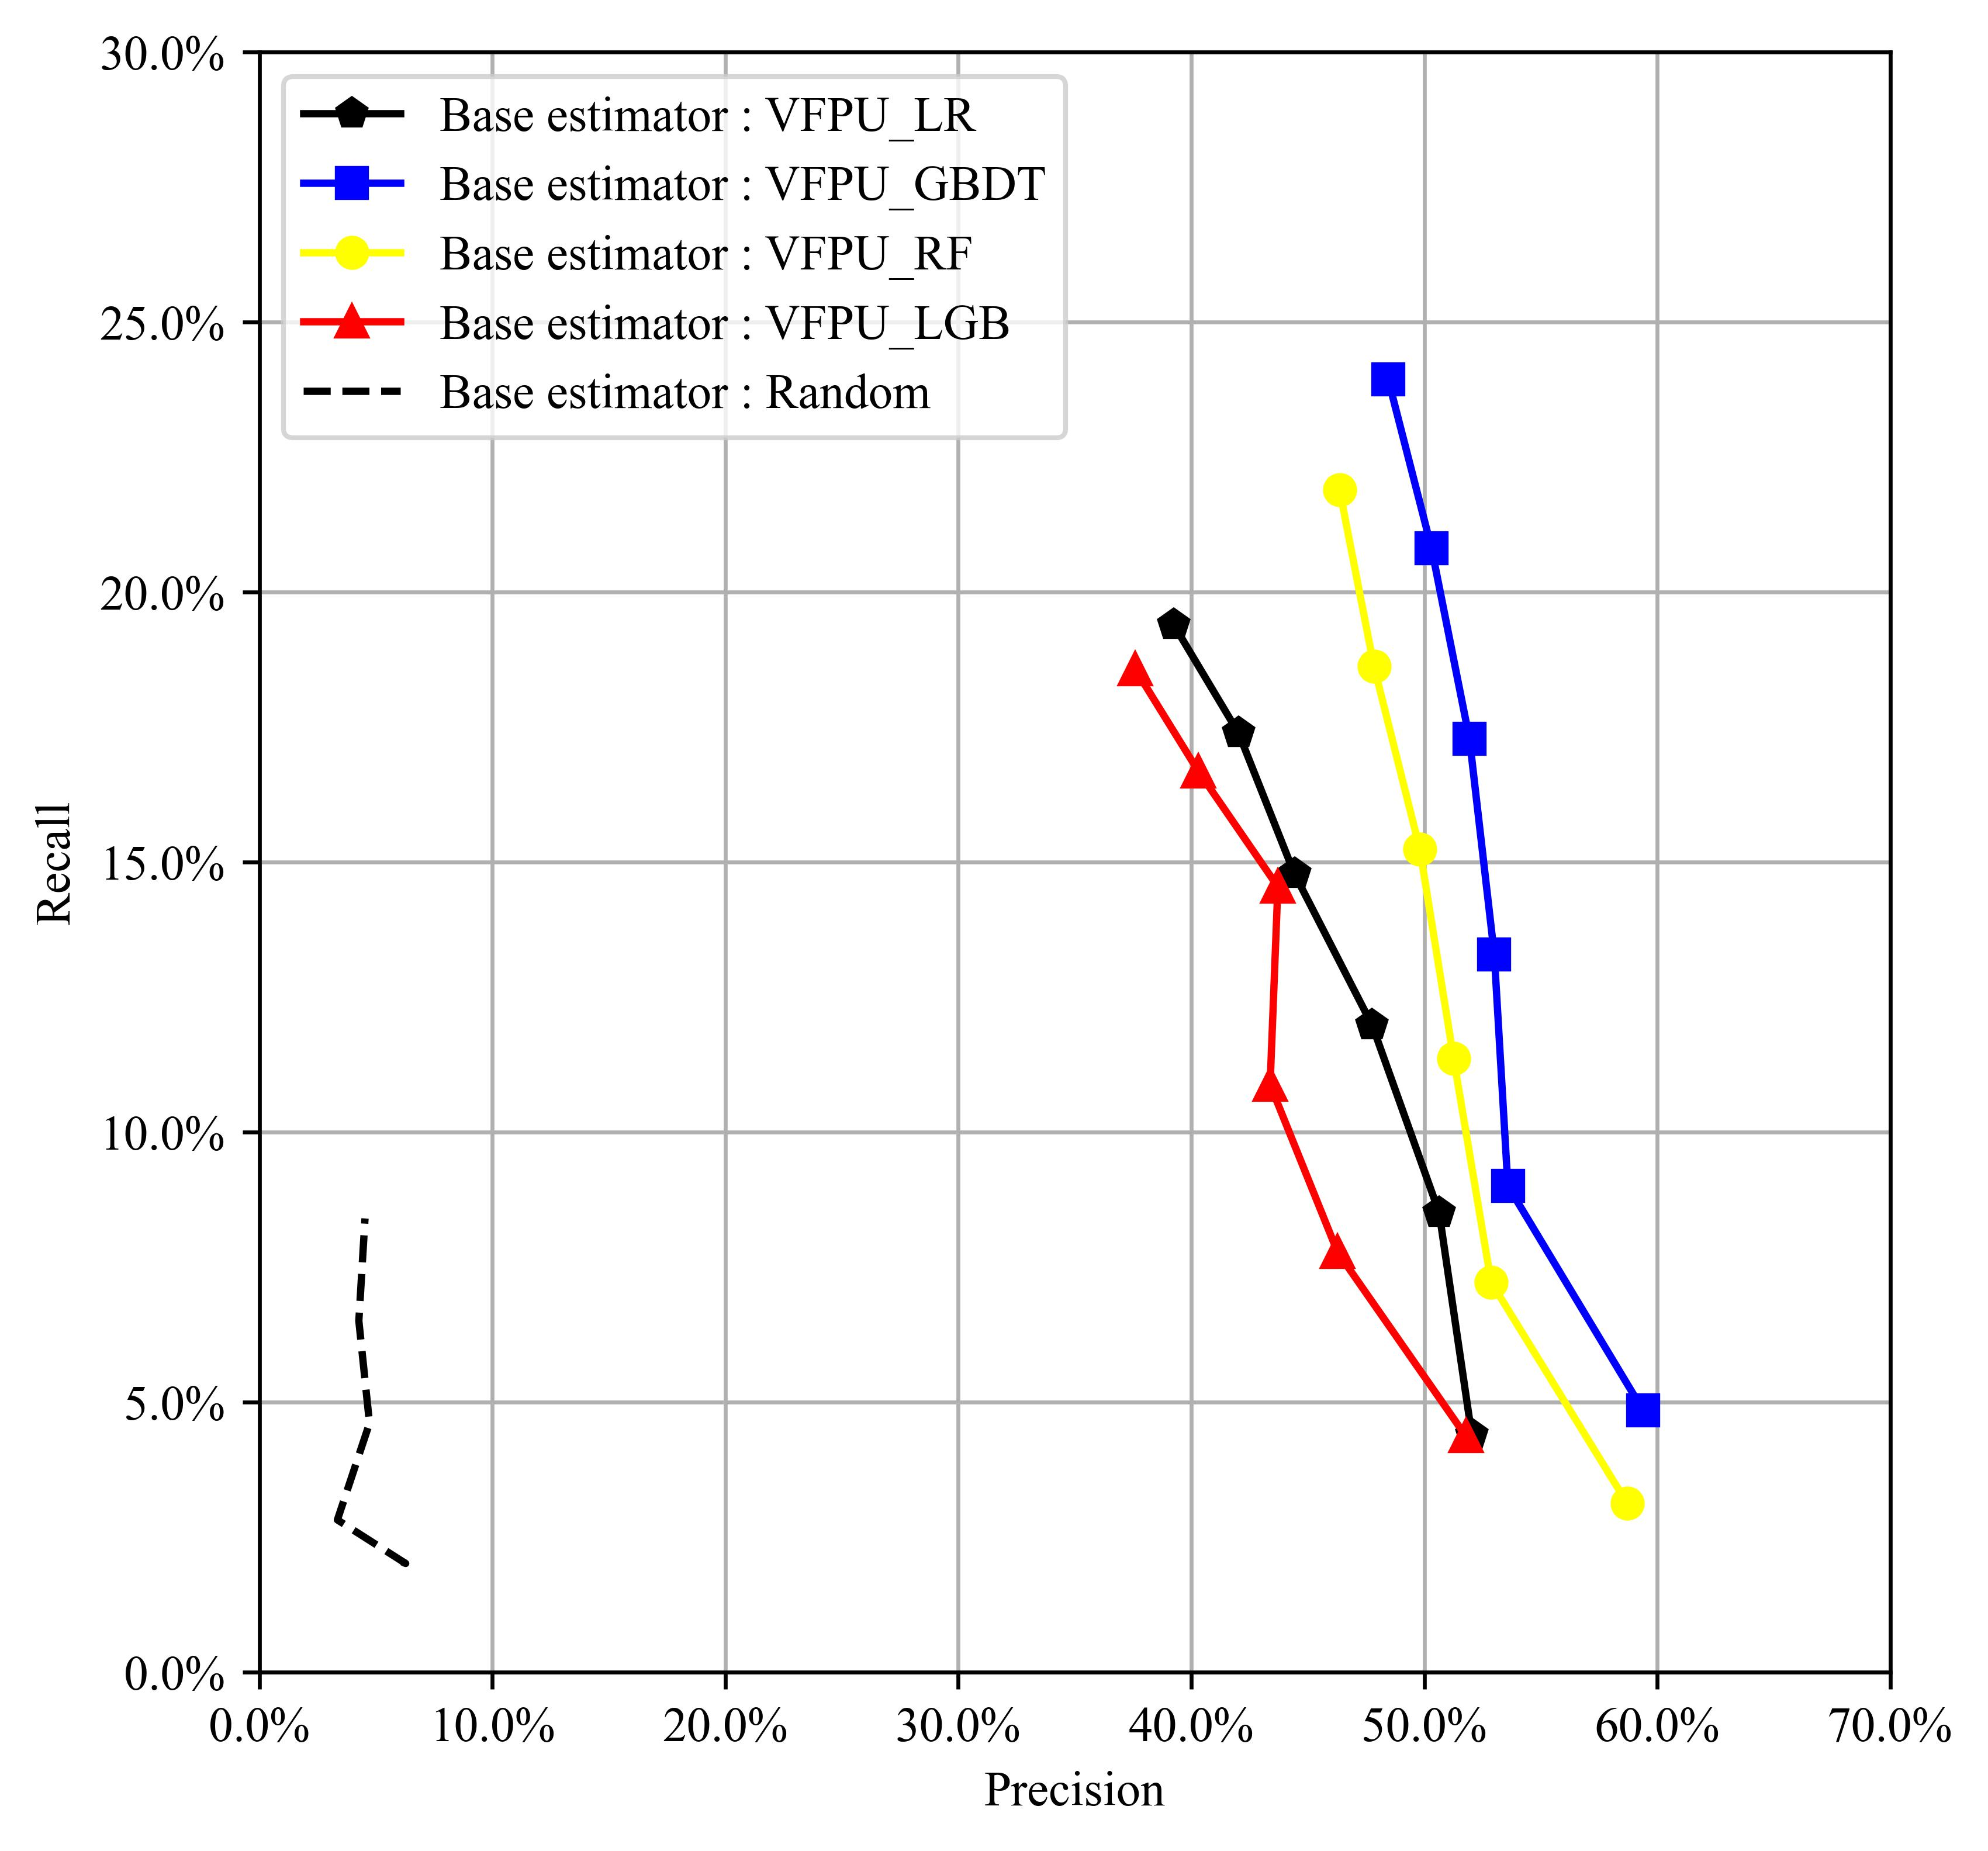
\includegraphics[width=0.95\textwidth,height=5.1cm]{chapters/imgs/Figure 2 (4) in JEPG format}
		\caption{Precision-Recall}
		\label{RQ2.1.sub4}
	\end{subfigure}
	
	\bicaption[\xiaosi 不同基学器在不同可靠正样本数量下的性能]{\wuhao 不同基学器在不同可靠正样本数量下的性能:(1)精度;(2)召回率;(3)F-score;(4)精度-召回率(Bank 数据集)}{\wuhao Performance of Different Base Estimators with Varying Reliable Positive Samples: (1) Precision; (2) Recall; (3) F-score; (4) Precision-Recall (The Bank Marketing Dataset)}
    \label{RQ2.1}
\end{figure}


\begin{figure}[!htbp]
	\centering
	\captionsetup{size=footnotesize}
	\begin{subfigure}{0.45\textwidth}
		\centering
		\captionsetup{skip=4pt}
		\captionsetup{size=scriptsize}
		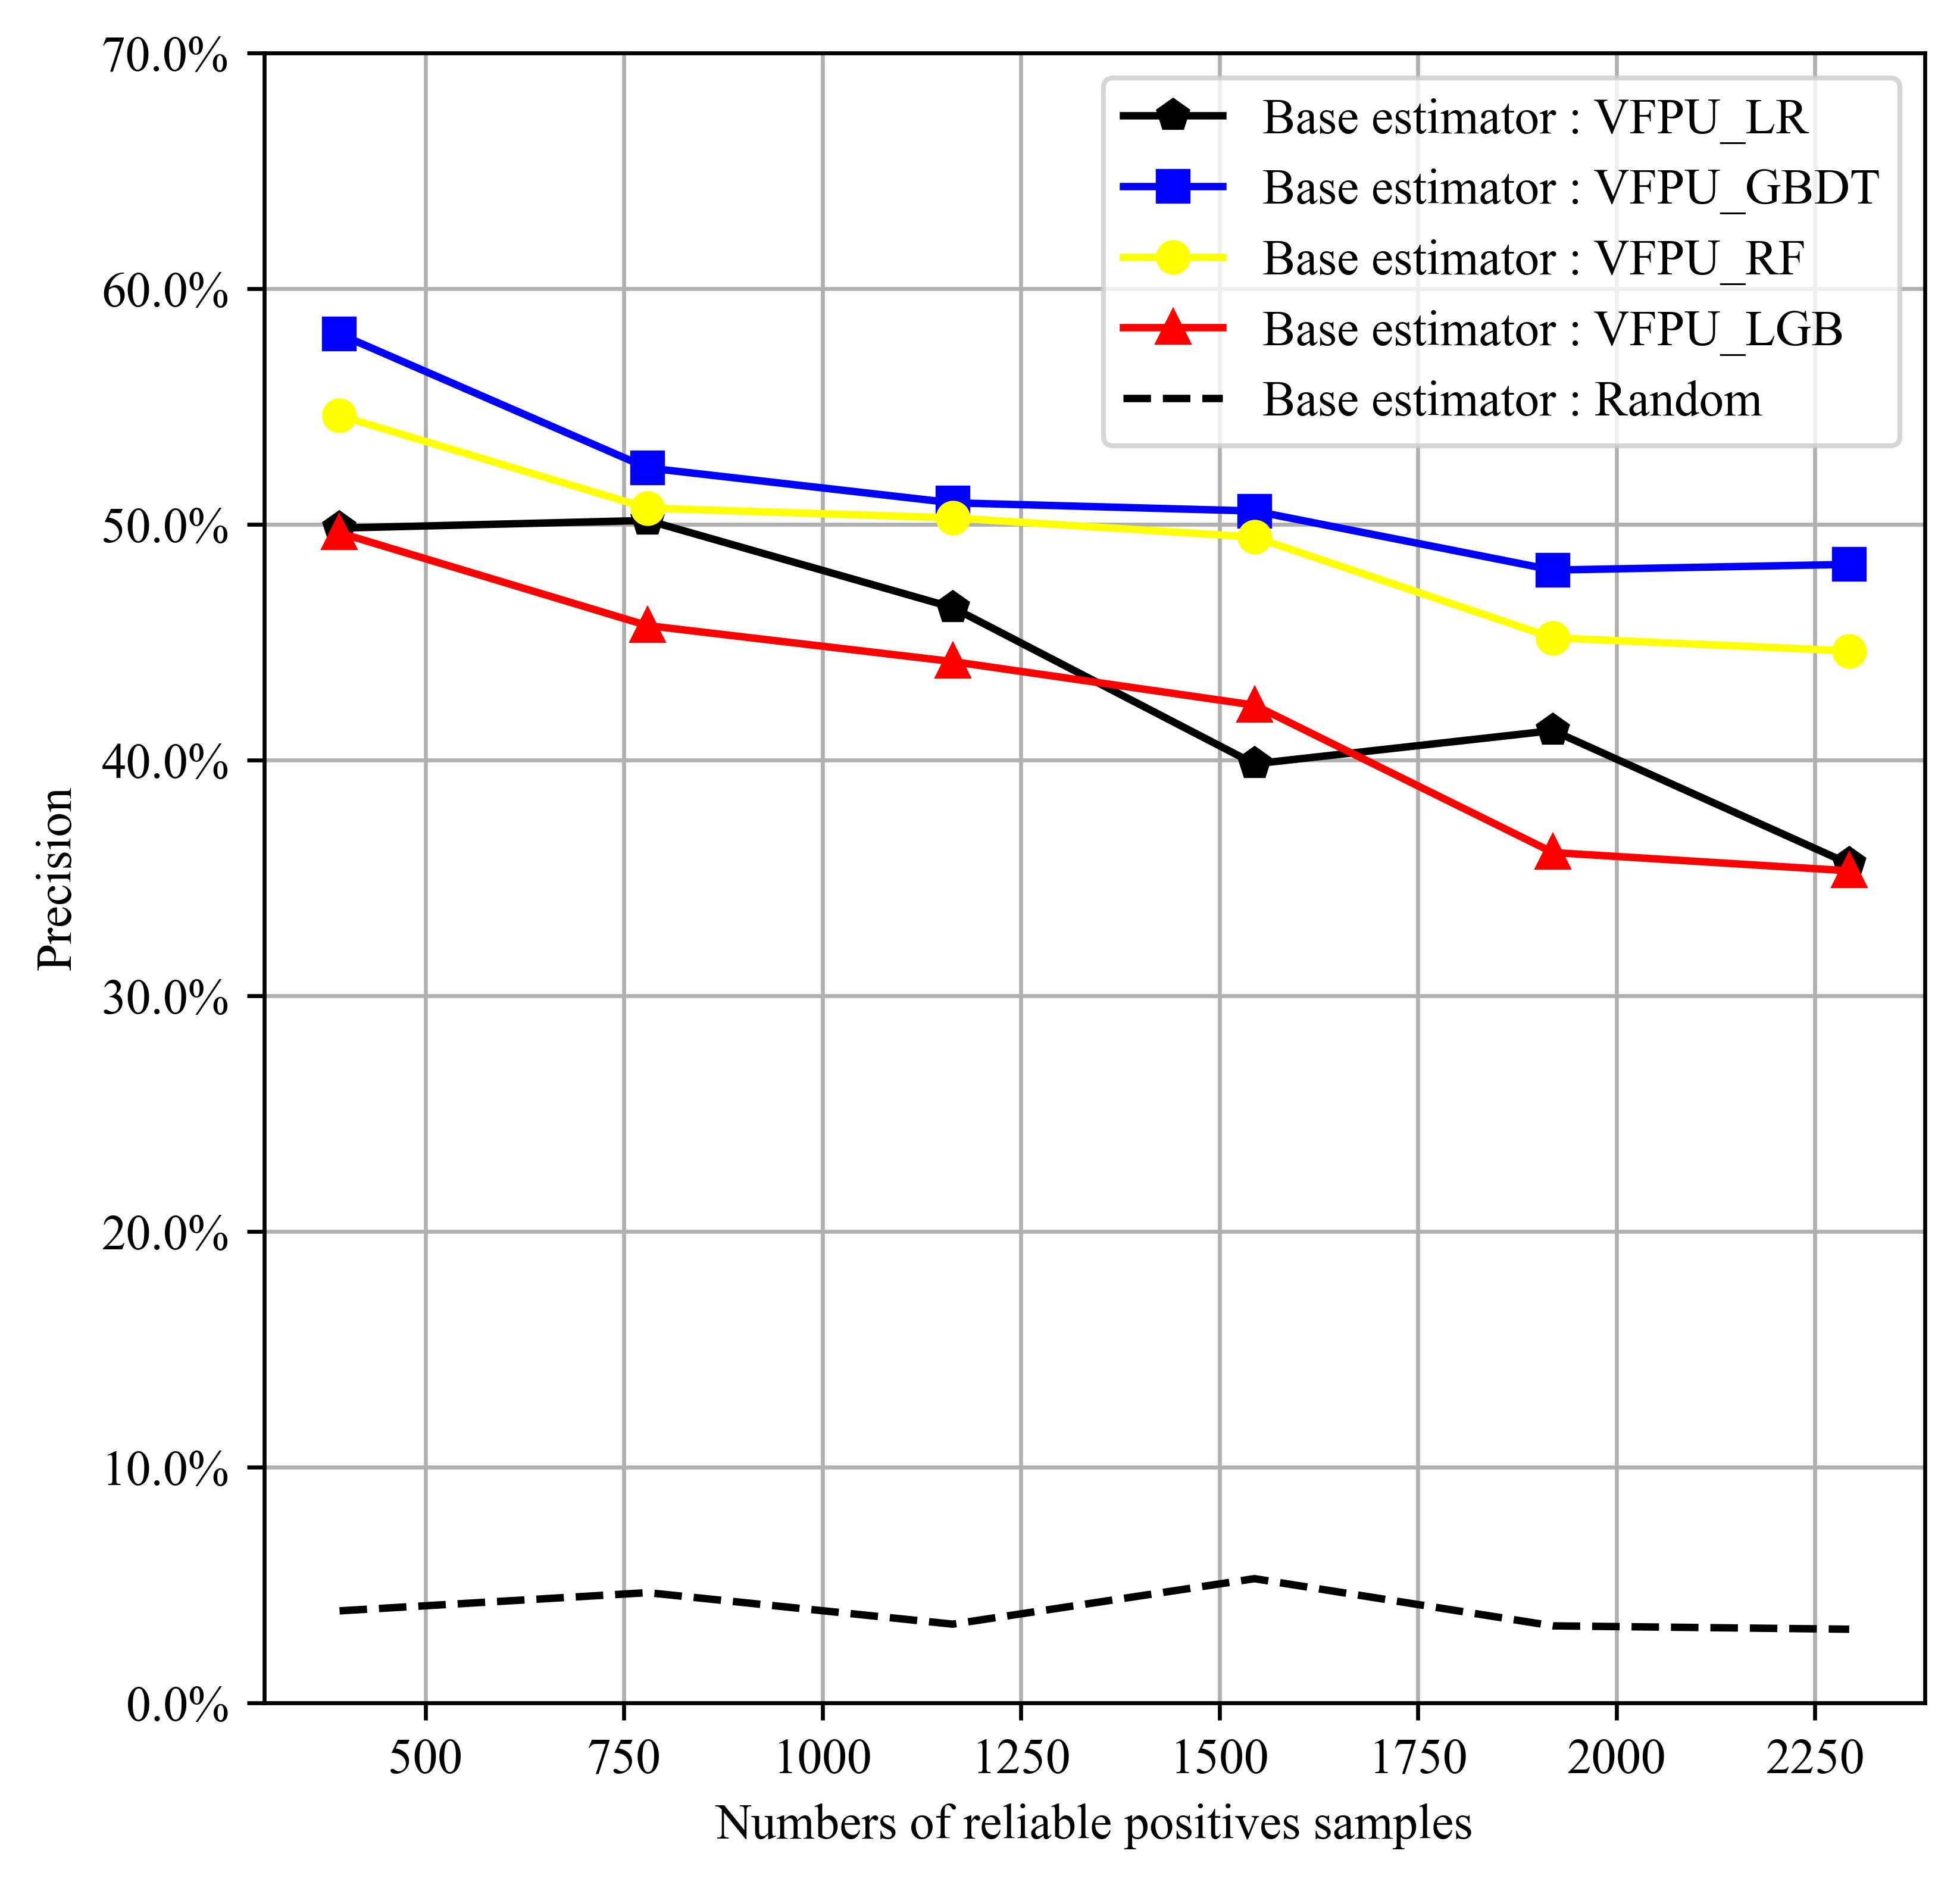
\includegraphics[width=0.9\textwidth,height=5.1cm]{chapters/imgs/Figure 3 (1) in JEPG format}
		\caption{Precision}
		\label{RQ2.2.sub1}
	\end{subfigure}
%\hfill
	\begin{subfigure}{0.45\textwidth}
		\centering
		\captionsetup{skip=4pt}
		\captionsetup{size=scriptsize}
		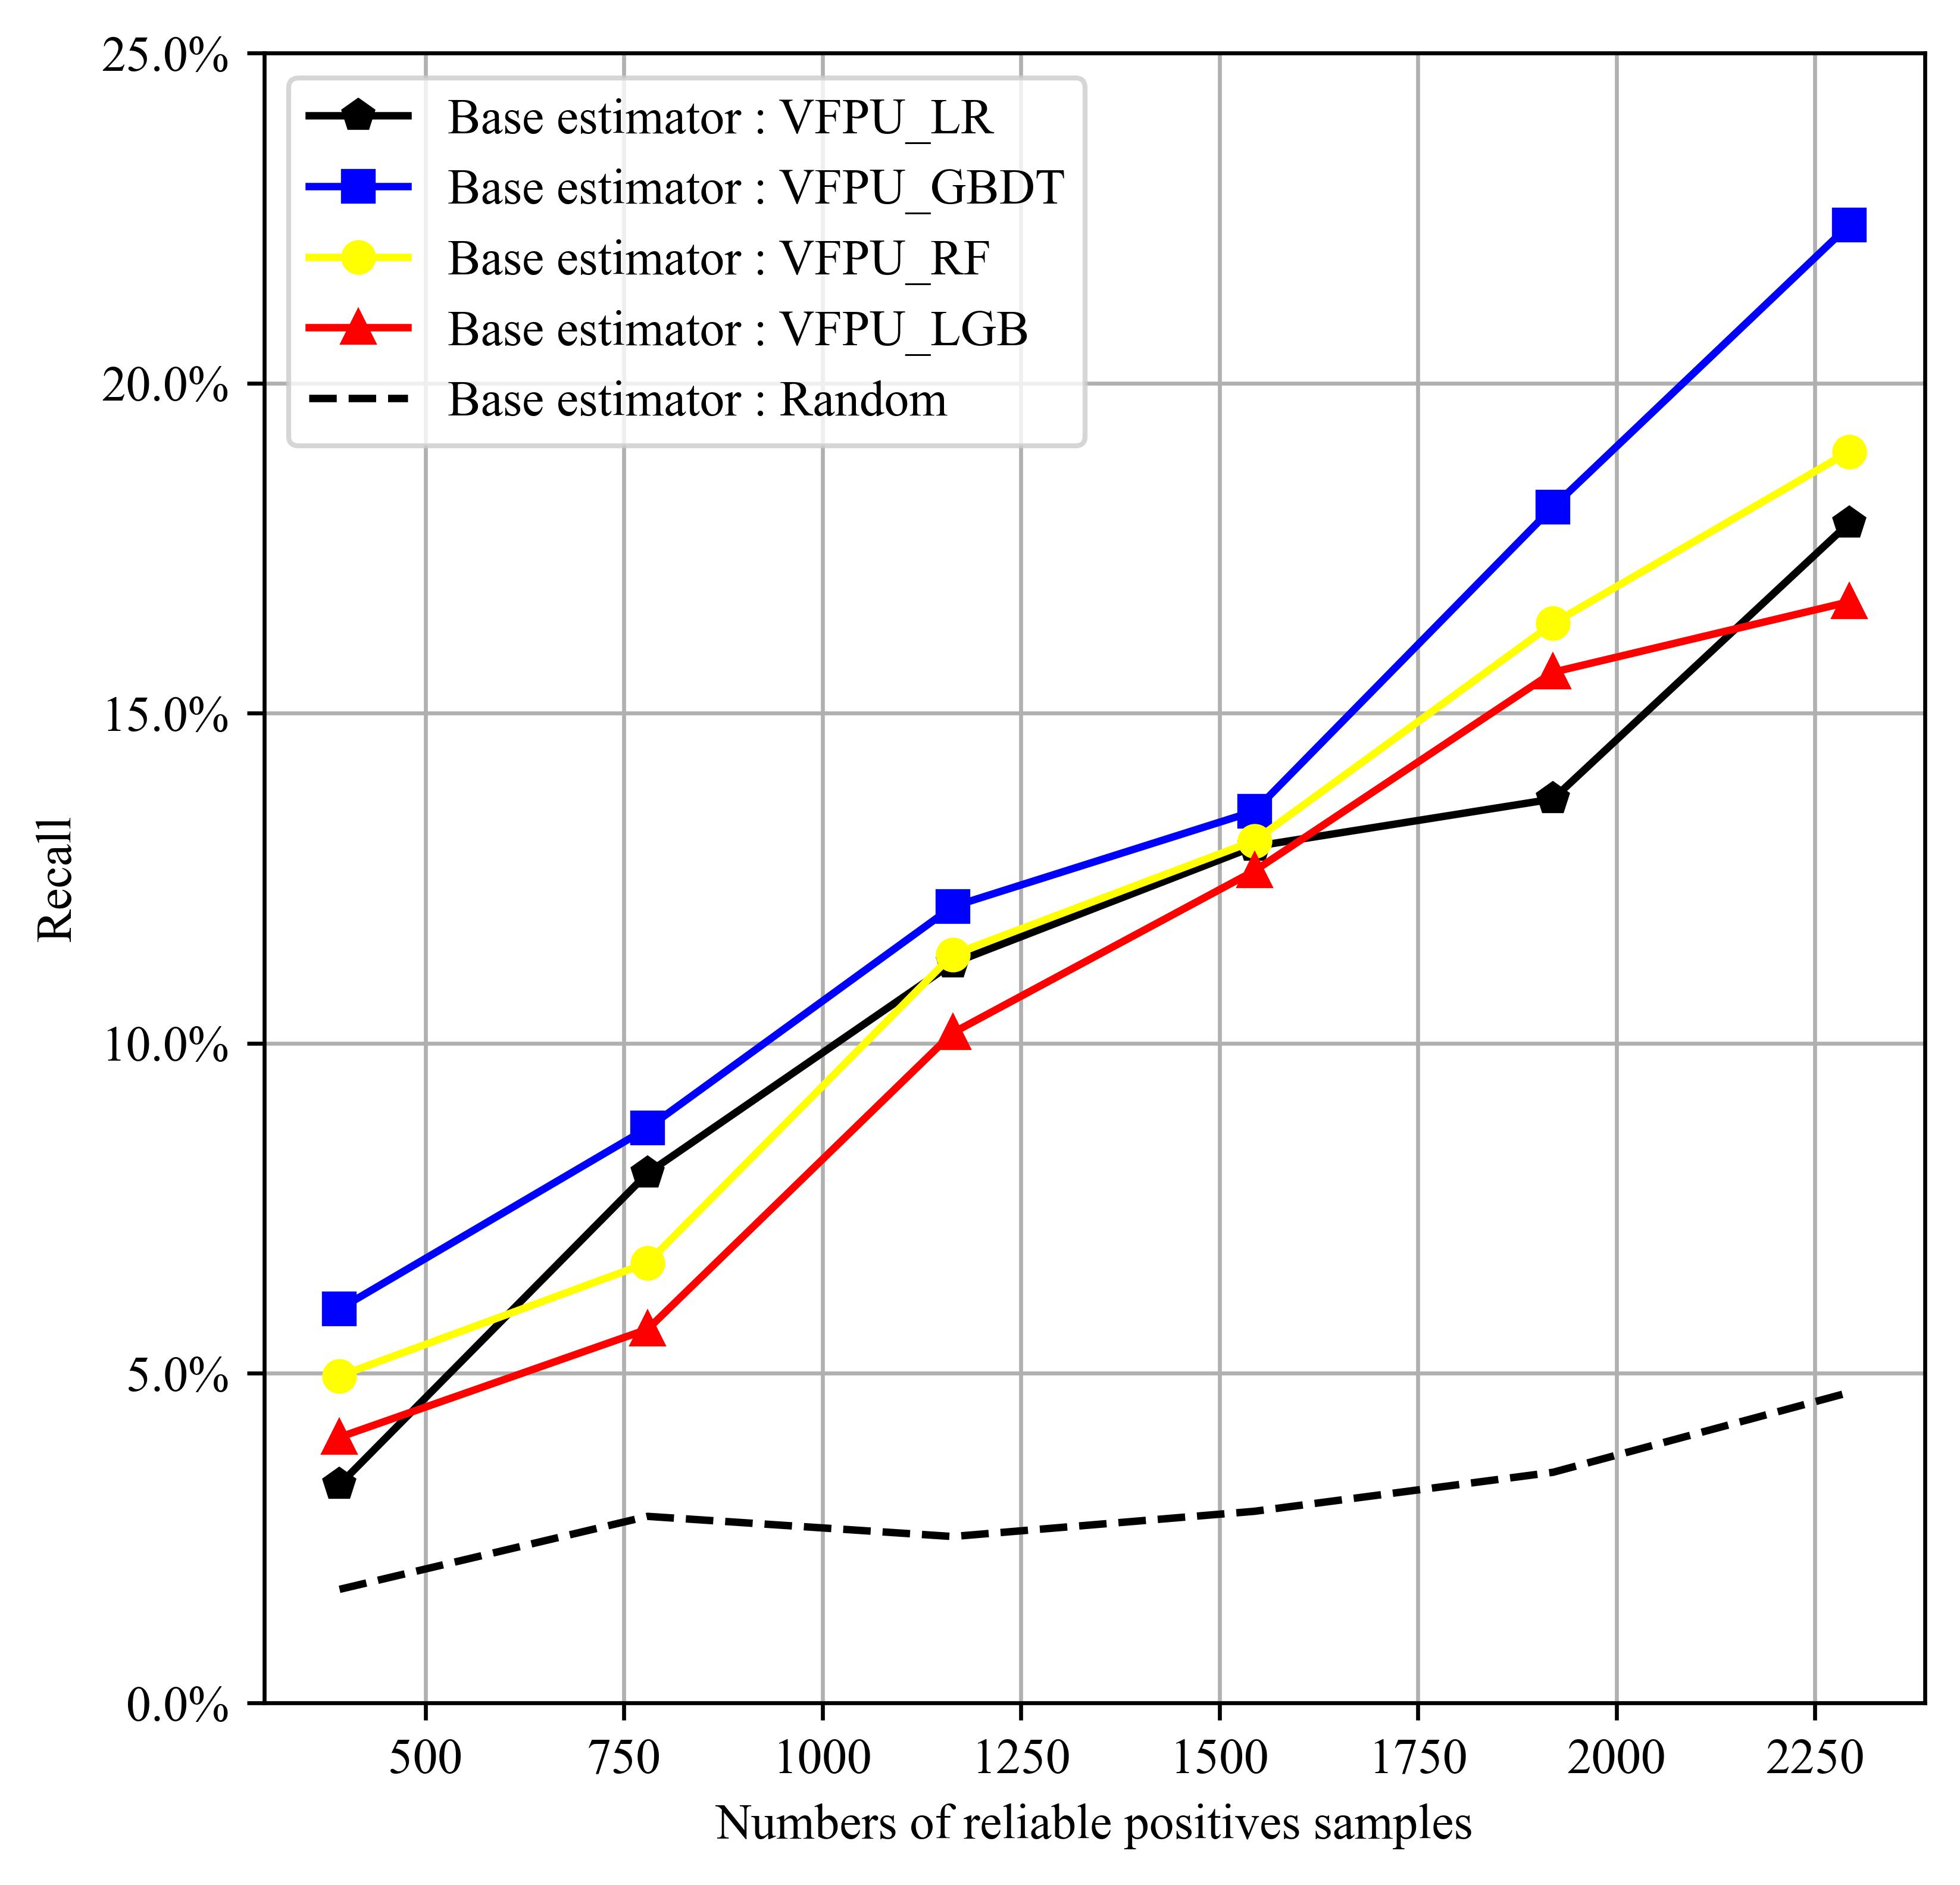
\includegraphics[width=0.9\textwidth,height=5.1cm]{chapters/imgs/Figure 3 (2) in JEPG format}
		\caption{Recall}
		\label{RQ2.2.sub2}
	\end{subfigure}
	
%	\vspace{0.05cm}
	
	\begin{subfigure}{0.45\textwidth}
		\centering
		\captionsetup{skip=4pt}
		\captionsetup{size=scriptsize}
		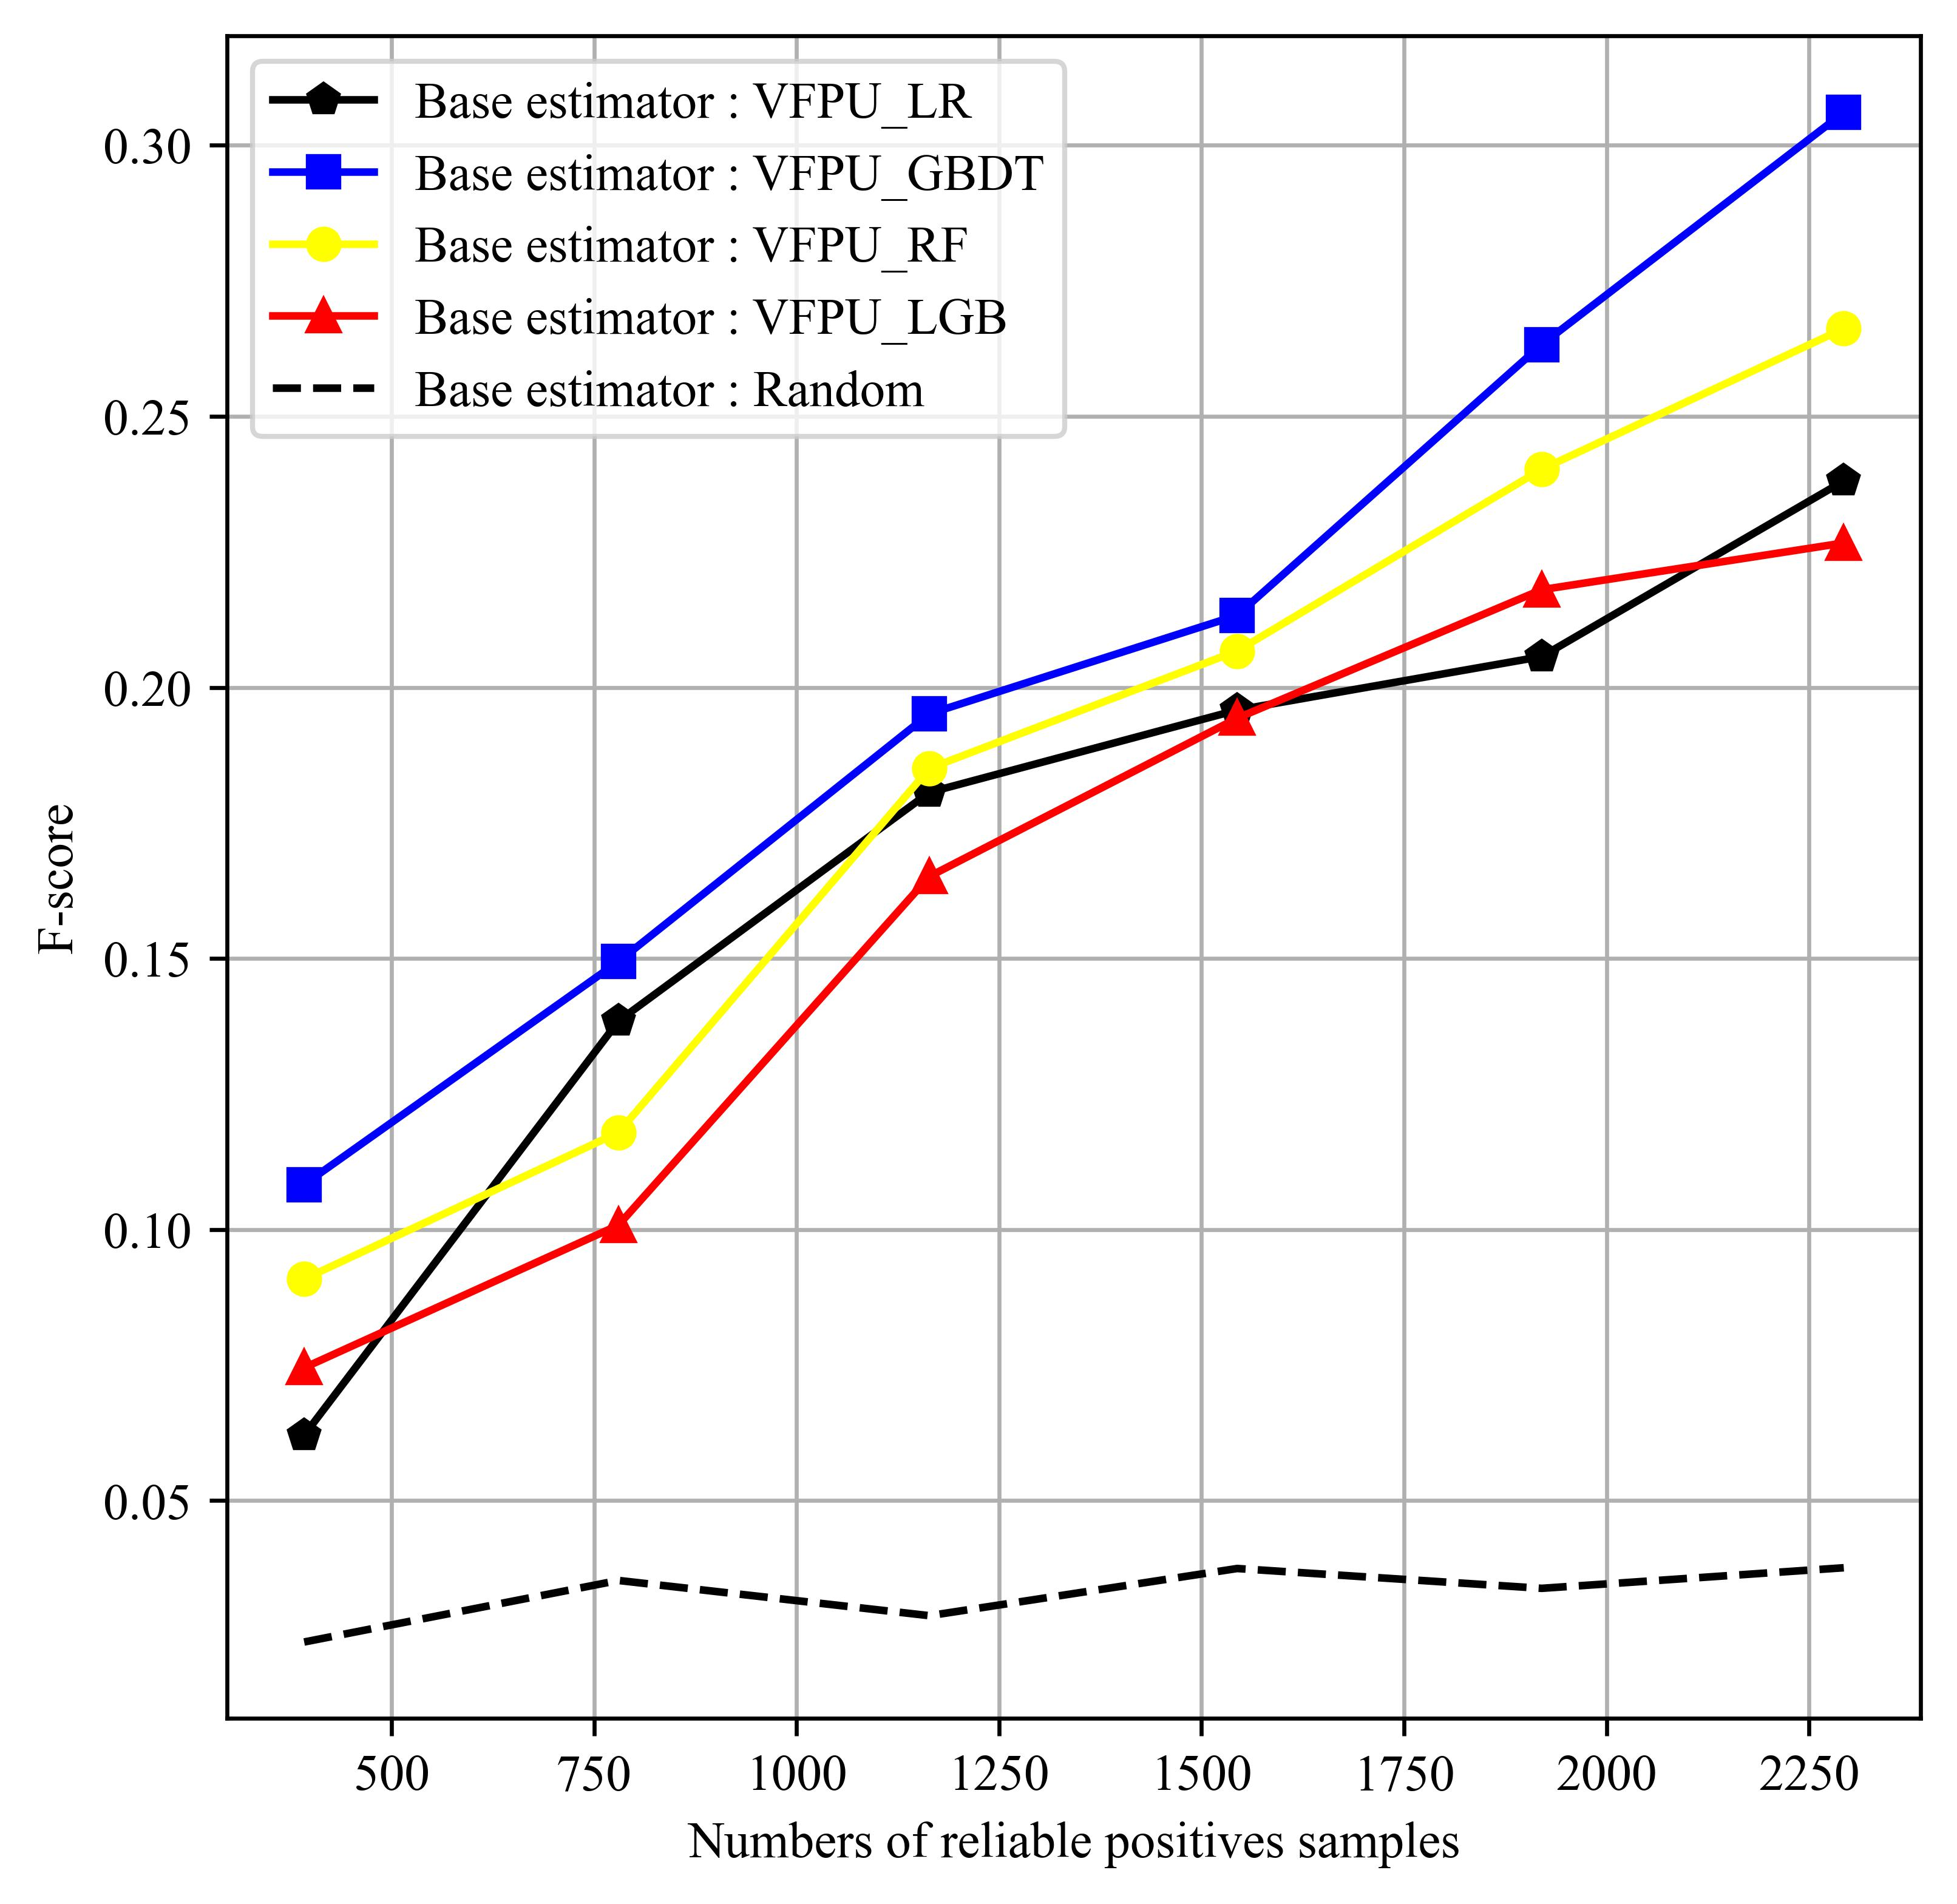
\includegraphics[width=0.9\textwidth,height=5.1cm]{chapters/imgs/Figure 3 (3) in JEPG format}
		\caption{F-score}
		\label{RQ2.2.sub3}
	\end{subfigure}
%\hfill
	\begin{subfigure}{0.45\textwidth}
		\centering
		\captionsetup{skip=4pt}
		\captionsetup{size=scriptsize}
		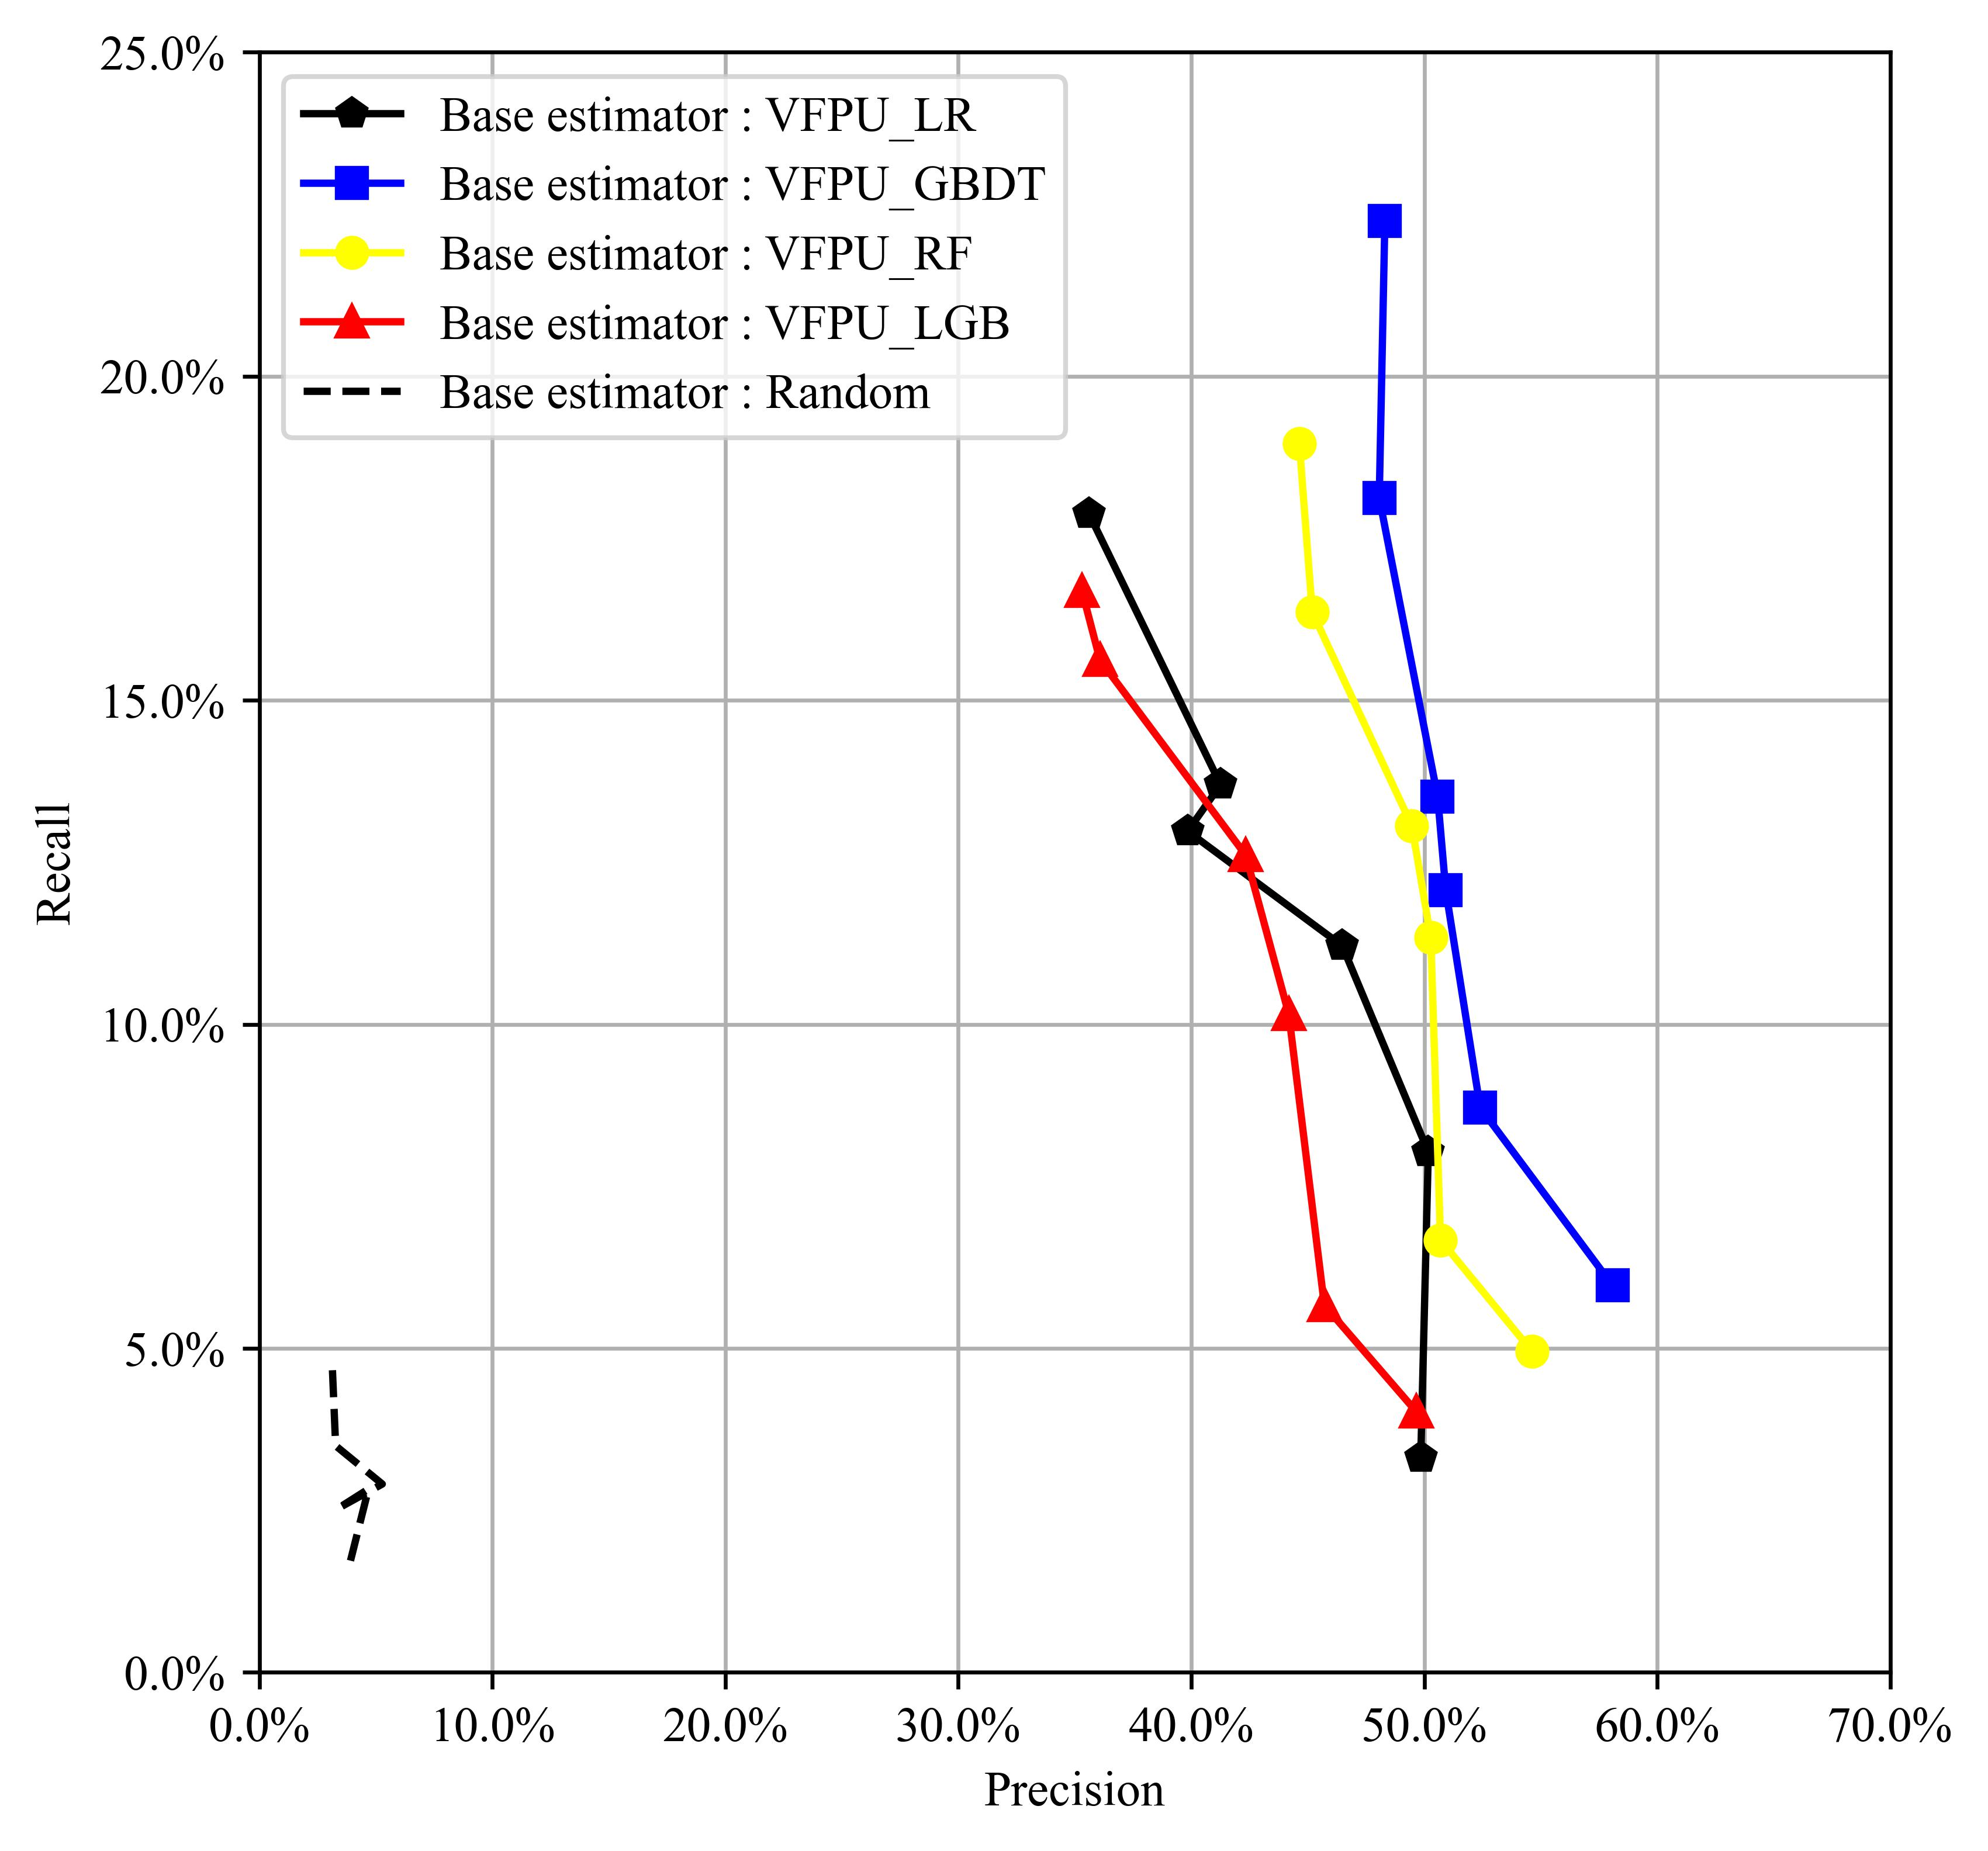
\includegraphics[width=0.9\textwidth,height=5.1cm]{chapters/imgs/Figure 3 (4) in JEPG format}
		\caption{Precision-Recall}
		\label{RQ2.2.sub4}
	\end{subfigure}
	
	\caption{Performance of Different Base Estimators with Varying Reliable Positive Samples: (1) Precision; (2) Recall; (3) F-score; (4) Precision-Recall (The Default of Credit Card Clients Dataset)}
	\bicaption[\xiaosi 不同基学器在不同可靠正样本数量下的性能]{\wuhao 不同基学器在不同可靠正样本数量下的性能:(1)精度;(2)召回率;(3)F-score;(4)精度-召回率(Credit 数据集)}{\wuhao Performance of Different Base Estimators with Varying Reliable Positive Samples: (1) Precision; (2) Recall; (3) F-score; (4) Precision-Recall (The Default of Credit Card Clients Dataset)}
    \label{RQ2.2}
\end{figure}

\begin{figure}[!htbp]
	\centering
	\captionsetup{size=footnotesize}
	\begin{subfigure}{0.45\textwidth}
		\centering
		\captionsetup{skip=2pt}
		\captionsetup{size=scriptsize}
		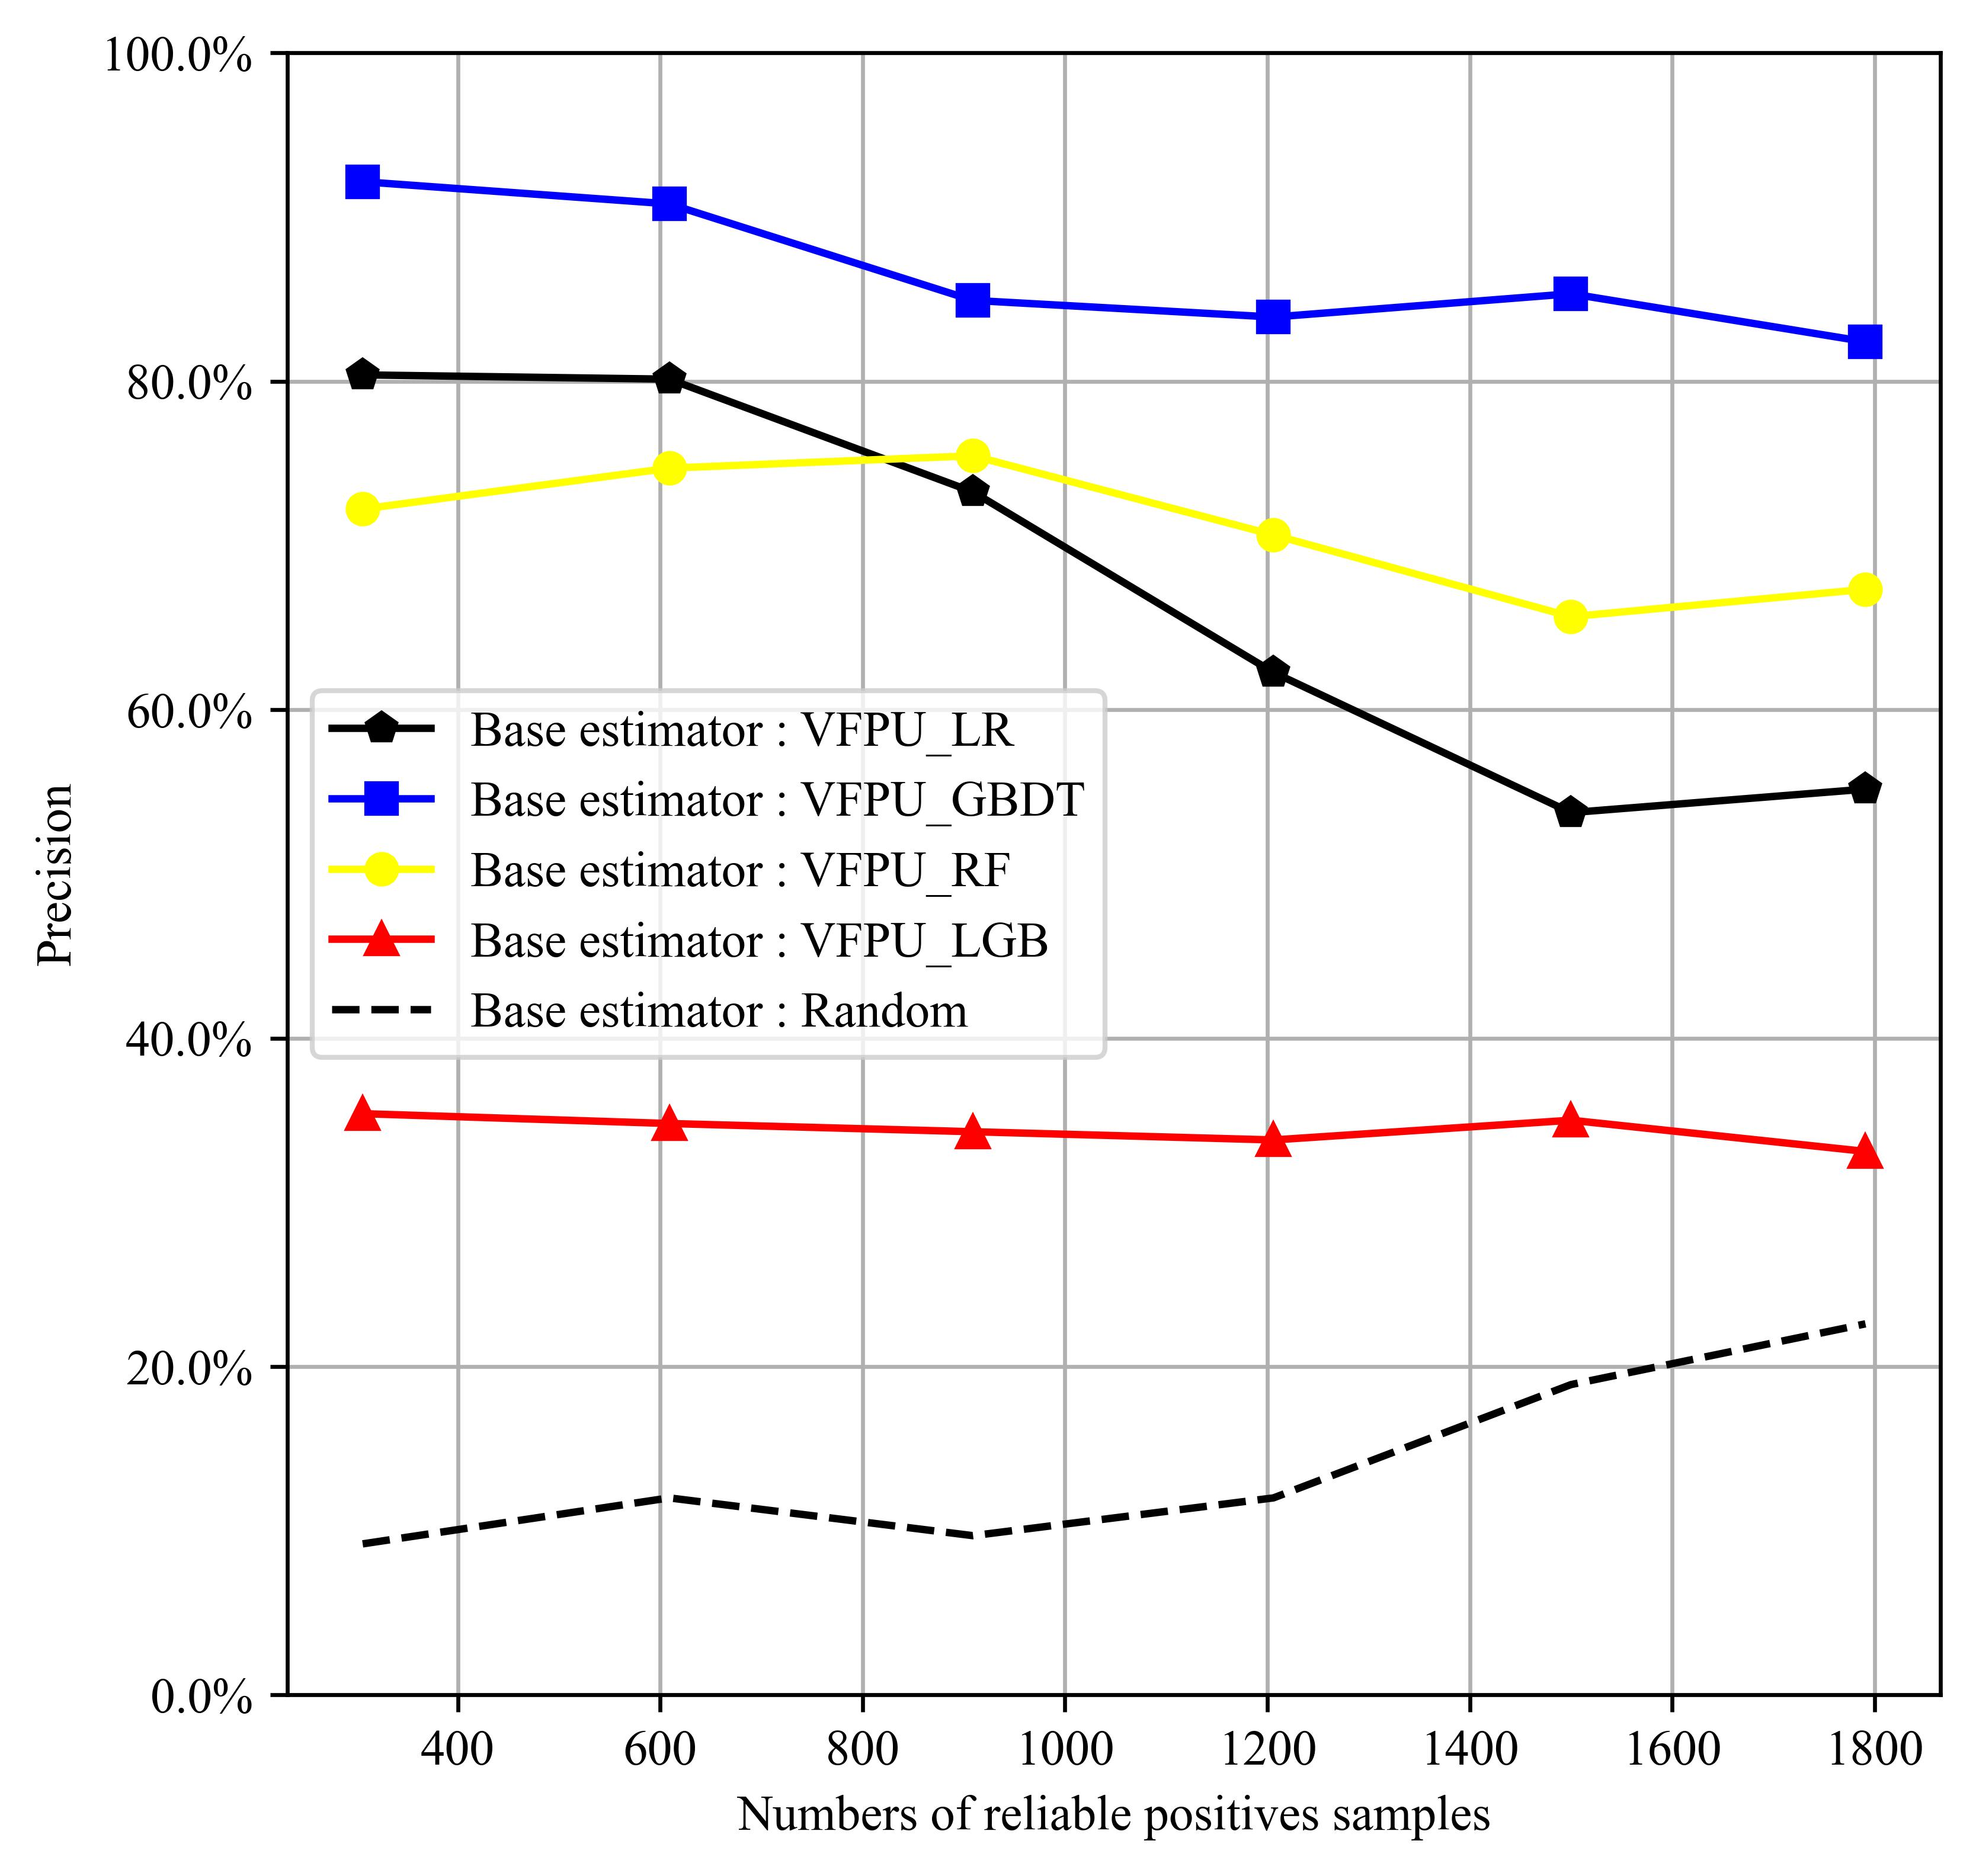
\includegraphics[width=0.9\textwidth,height=5.1cm]{chapters/imgs/Figure 4 (1) in JEPG format}
		\caption{Precision}
		\label{RQ2.3.sub1}
	\end{subfigure}
%\hfill
	\begin{subfigure}{0.45\textwidth}
		\centering
		\captionsetup{skip=2pt}
		\captionsetup{size=scriptsize}
		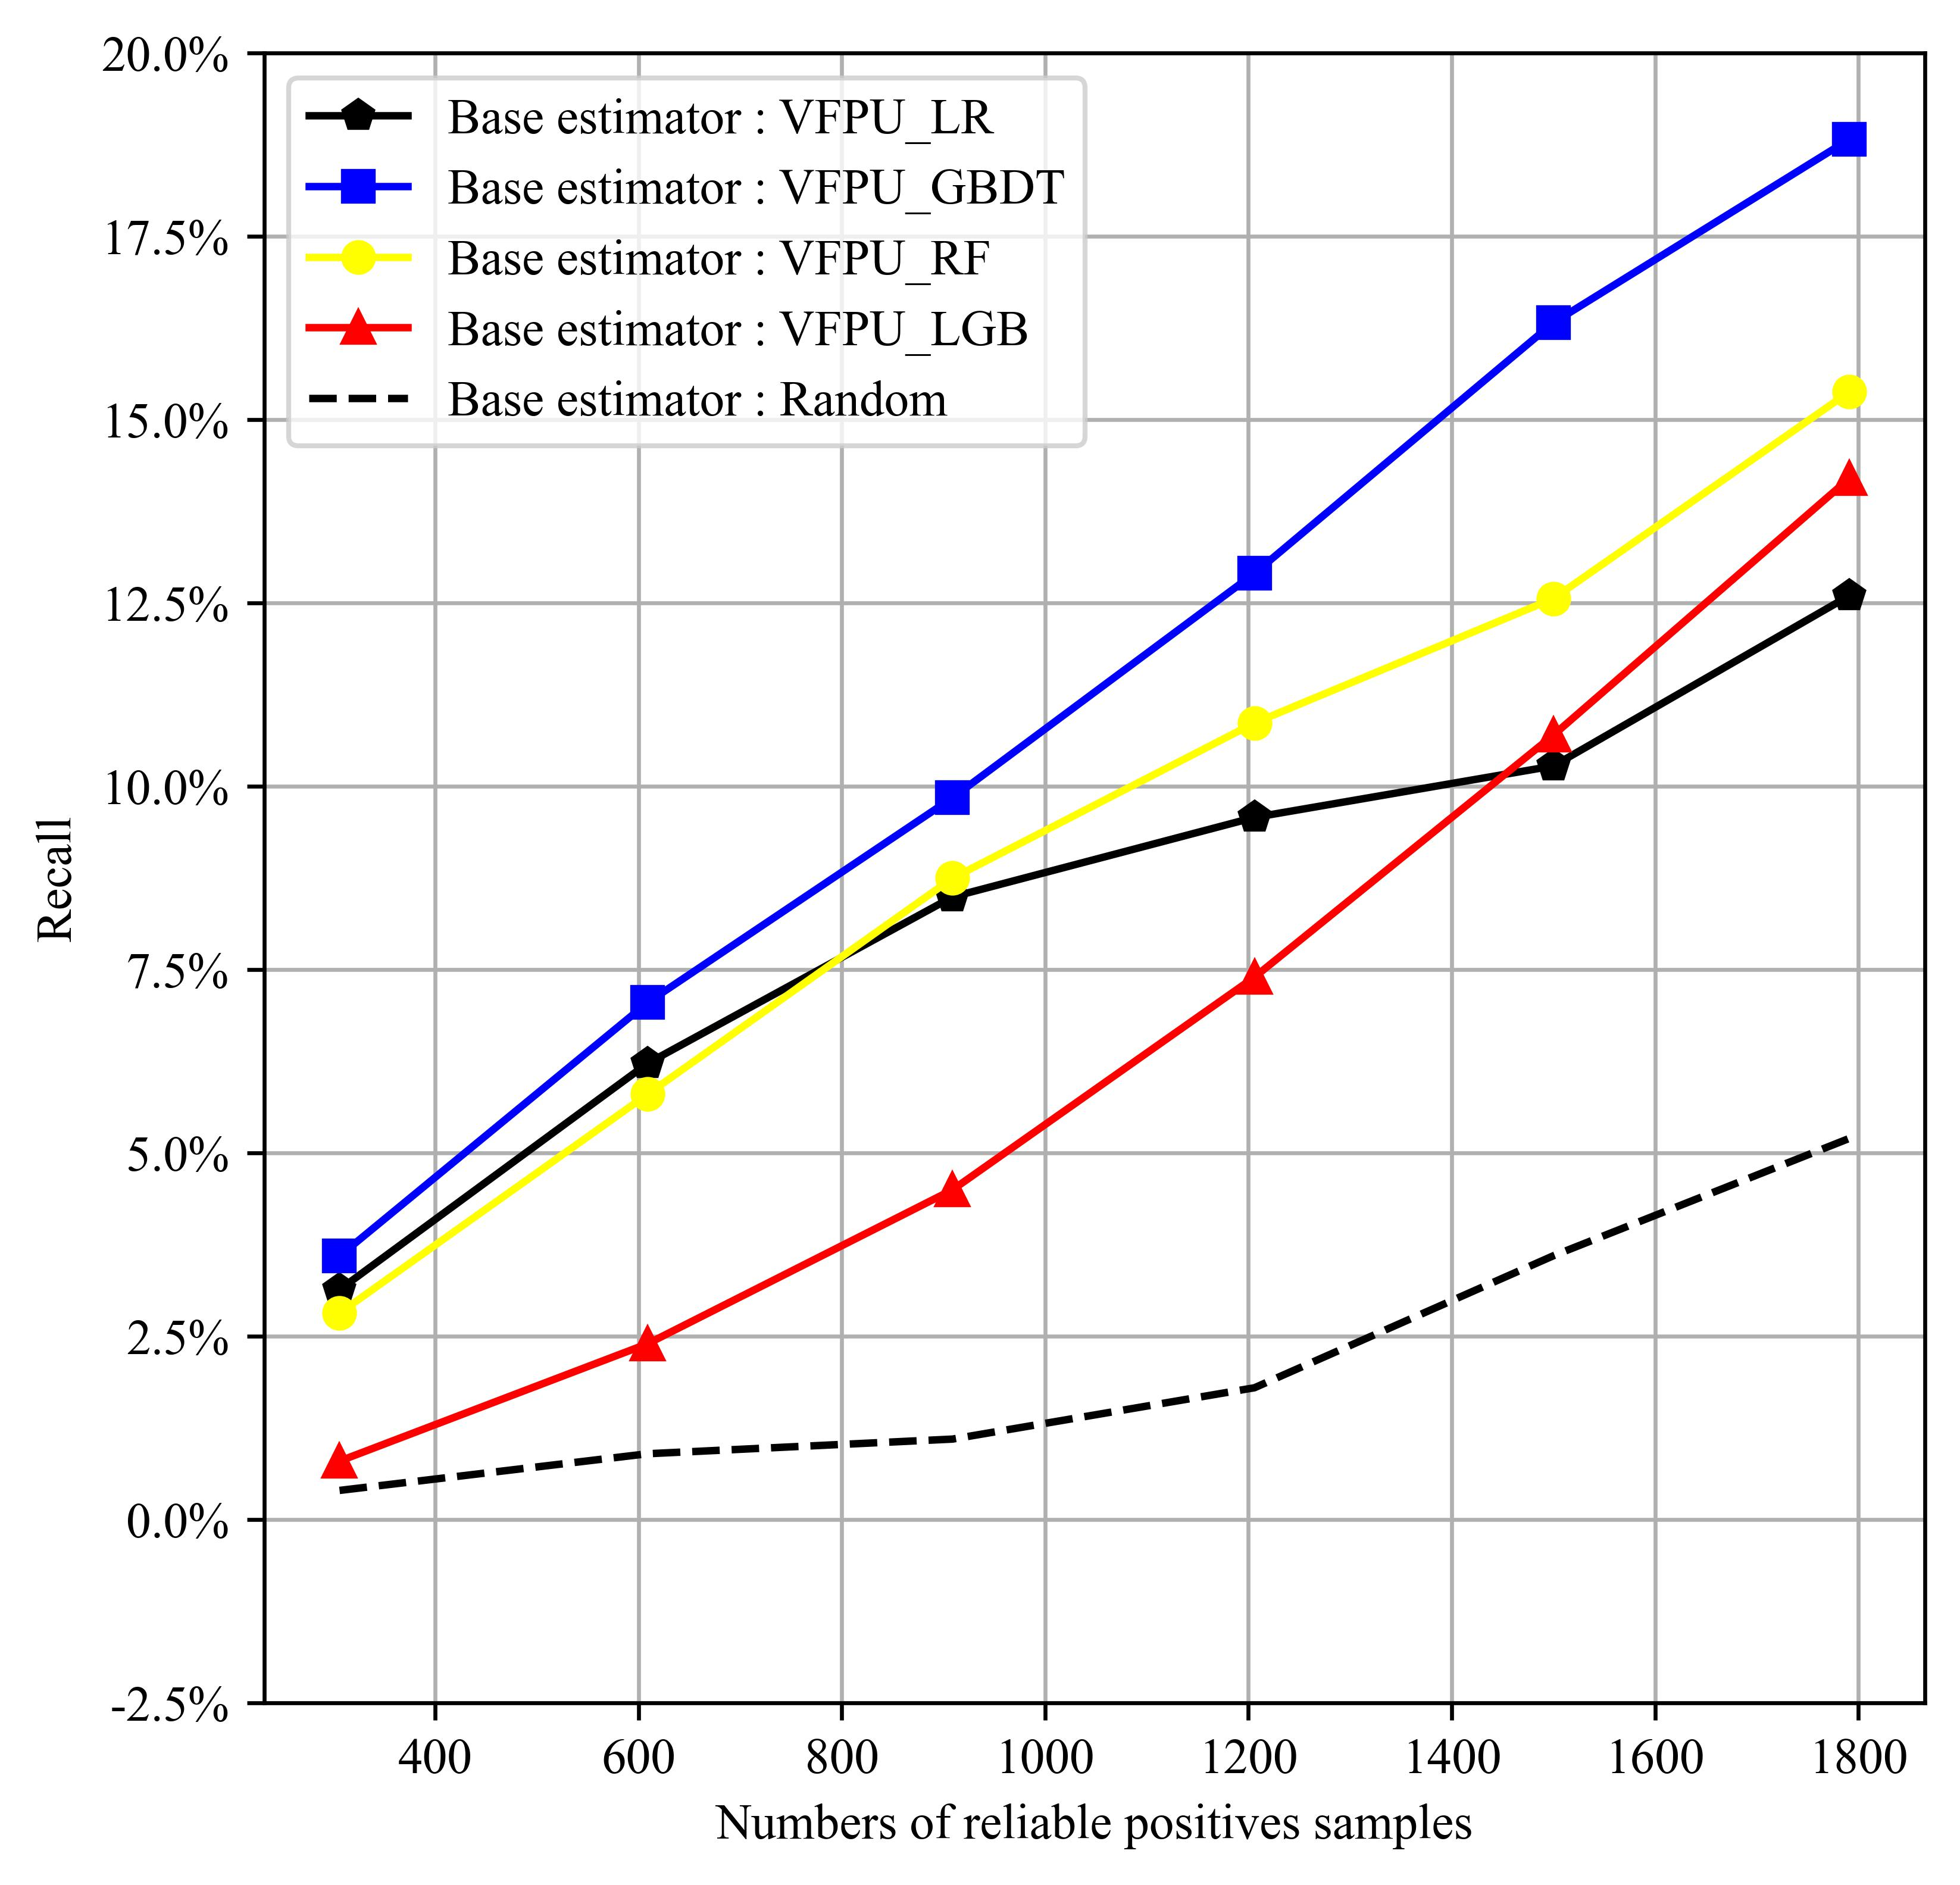
\includegraphics[width=0.9\textwidth,height=5.1cm]{chapters/imgs/Figure 4 (2) in JEPG format}
		\caption{Recall}
		\label{RQ2.3.sub2}
	\end{subfigure}
	
%	\vspace{0.05cm}
	
	\begin{subfigure}{0.45\textwidth}
		\centering
		\captionsetup{skip=2pt}
		\captionsetup{size=scriptsize}
		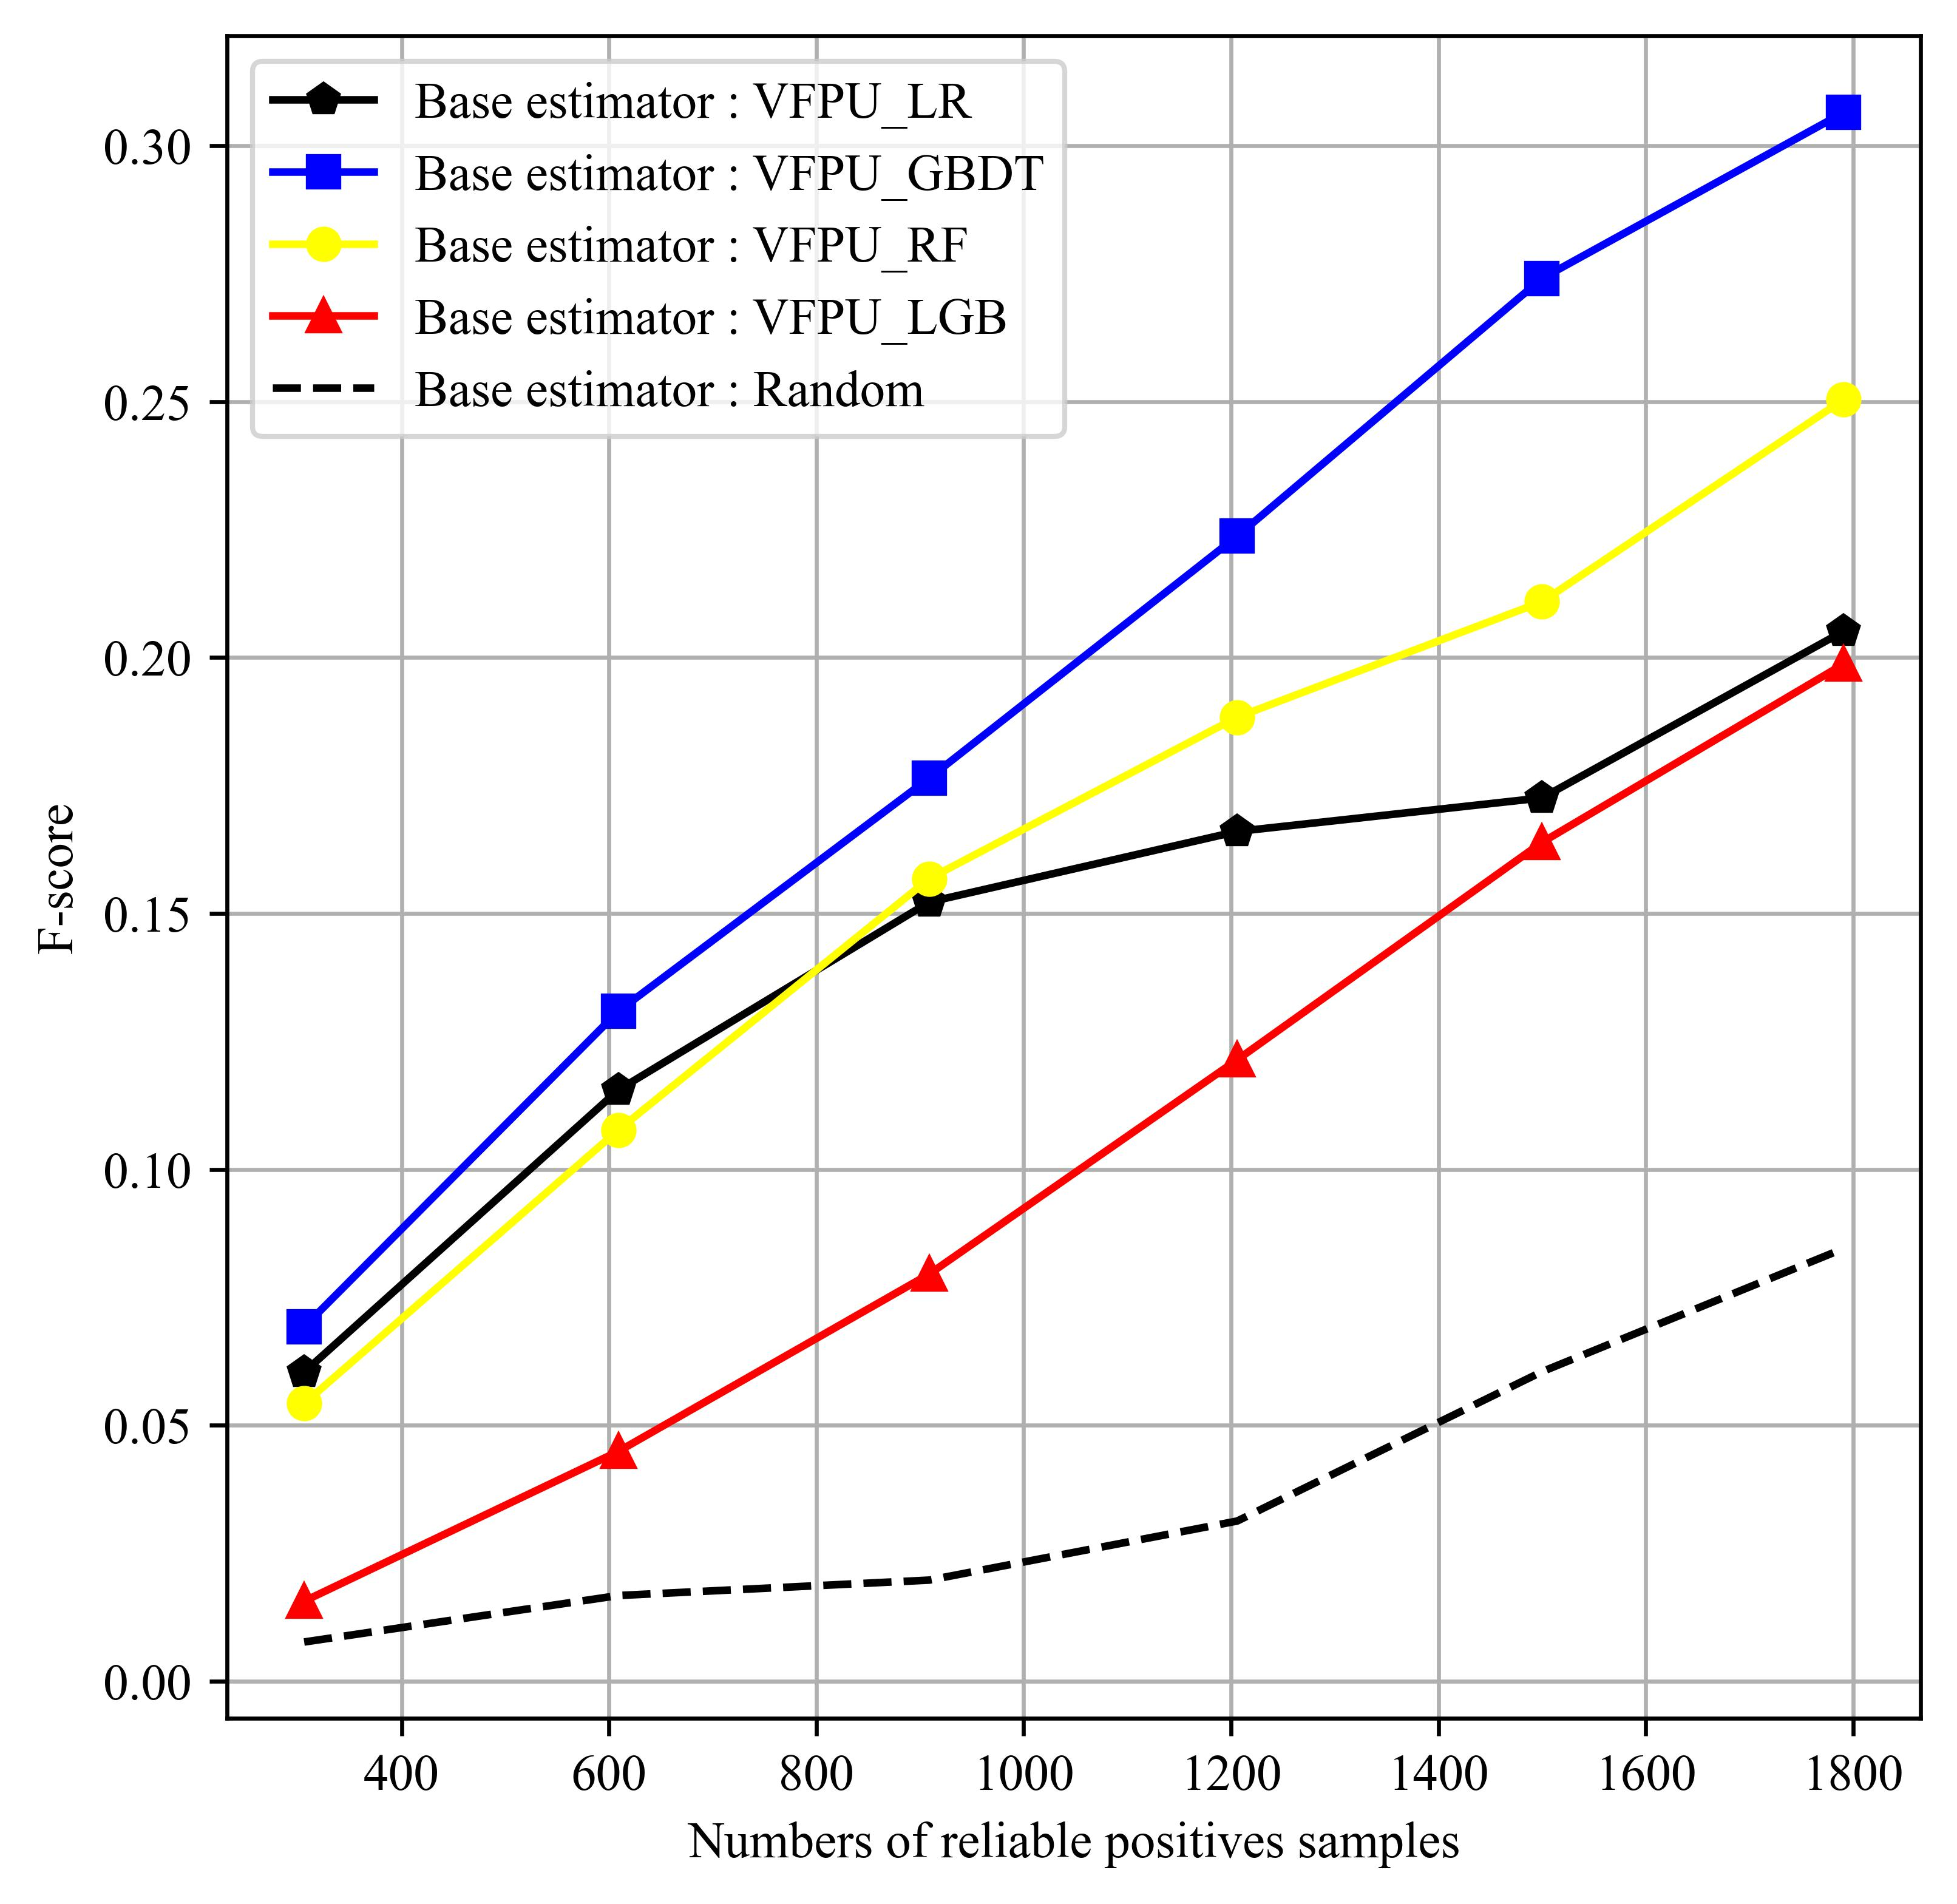
\includegraphics[width=0.9\textwidth,height=5.1cm]{chapters/imgs/Figure 4 (3) in JEPG format}
		\caption{F-score}
		\label{RQ2.3.sub3}
	\end{subfigure}
%\hfill
	\begin{subfigure}{0.45\textwidth}
		\centering
		\captionsetup{skip=2pt}
		\captionsetup{size=scriptsize}
		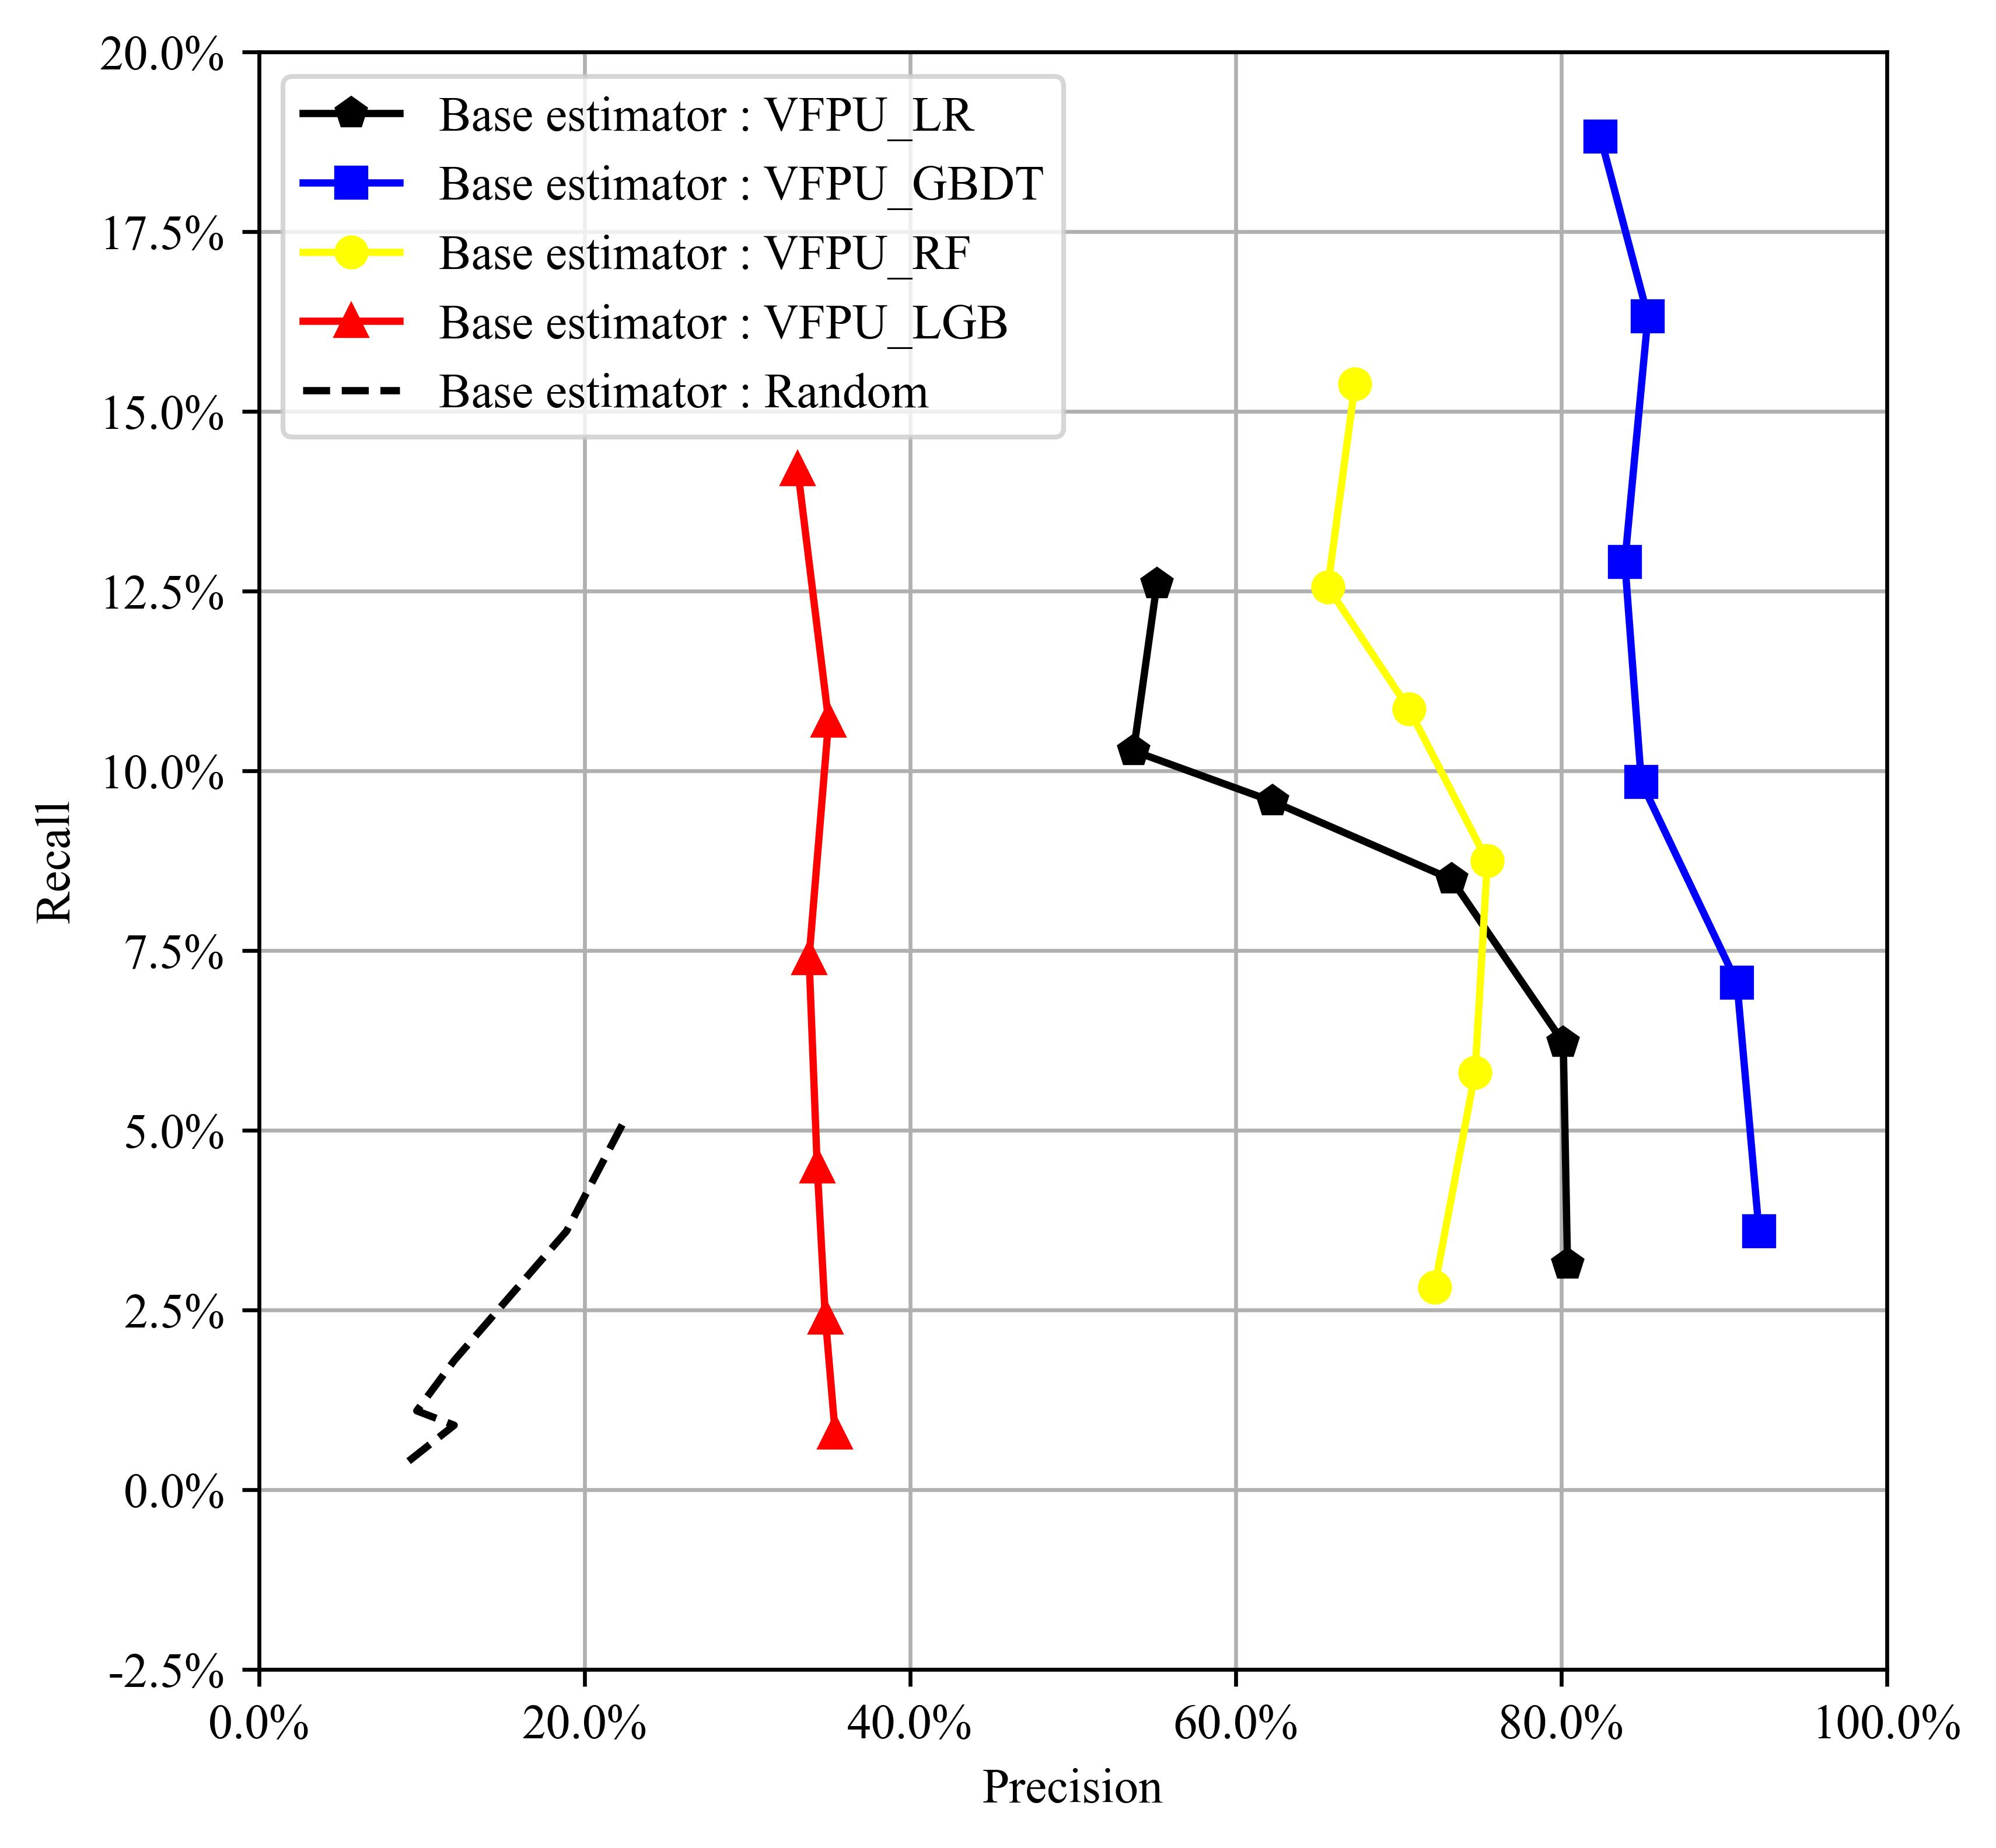
\includegraphics[width=0.9\textwidth,height=5.1cm]{chapters/imgs/Figure 4 (4) in JEPG format}
		\caption{Precision-Recall}
		\label{RQ2.3.sub4}
	\end{subfigure}
	\bicaption[\xiaosi 不同基学器在不同可靠正样本数量下的性能]{\wuhao 不同基学器在不同可靠正样本数量下的性能:(1)精度;(2)召回率;(3)F-score;(4)精度-召回率(Census 数据集)}{\wuhao Performance of Different Base Estimators with Varying Reliable Positive Samples: (1) Precision; (2) Recall; (3) F-score; (4) Precision-Recall (The Adult Census Dataset)}
    \label{RQ2.3}
\end{figure}

\begin{figure}[!htbp]
	\centering
	\captionsetup{size=footnotesize}
	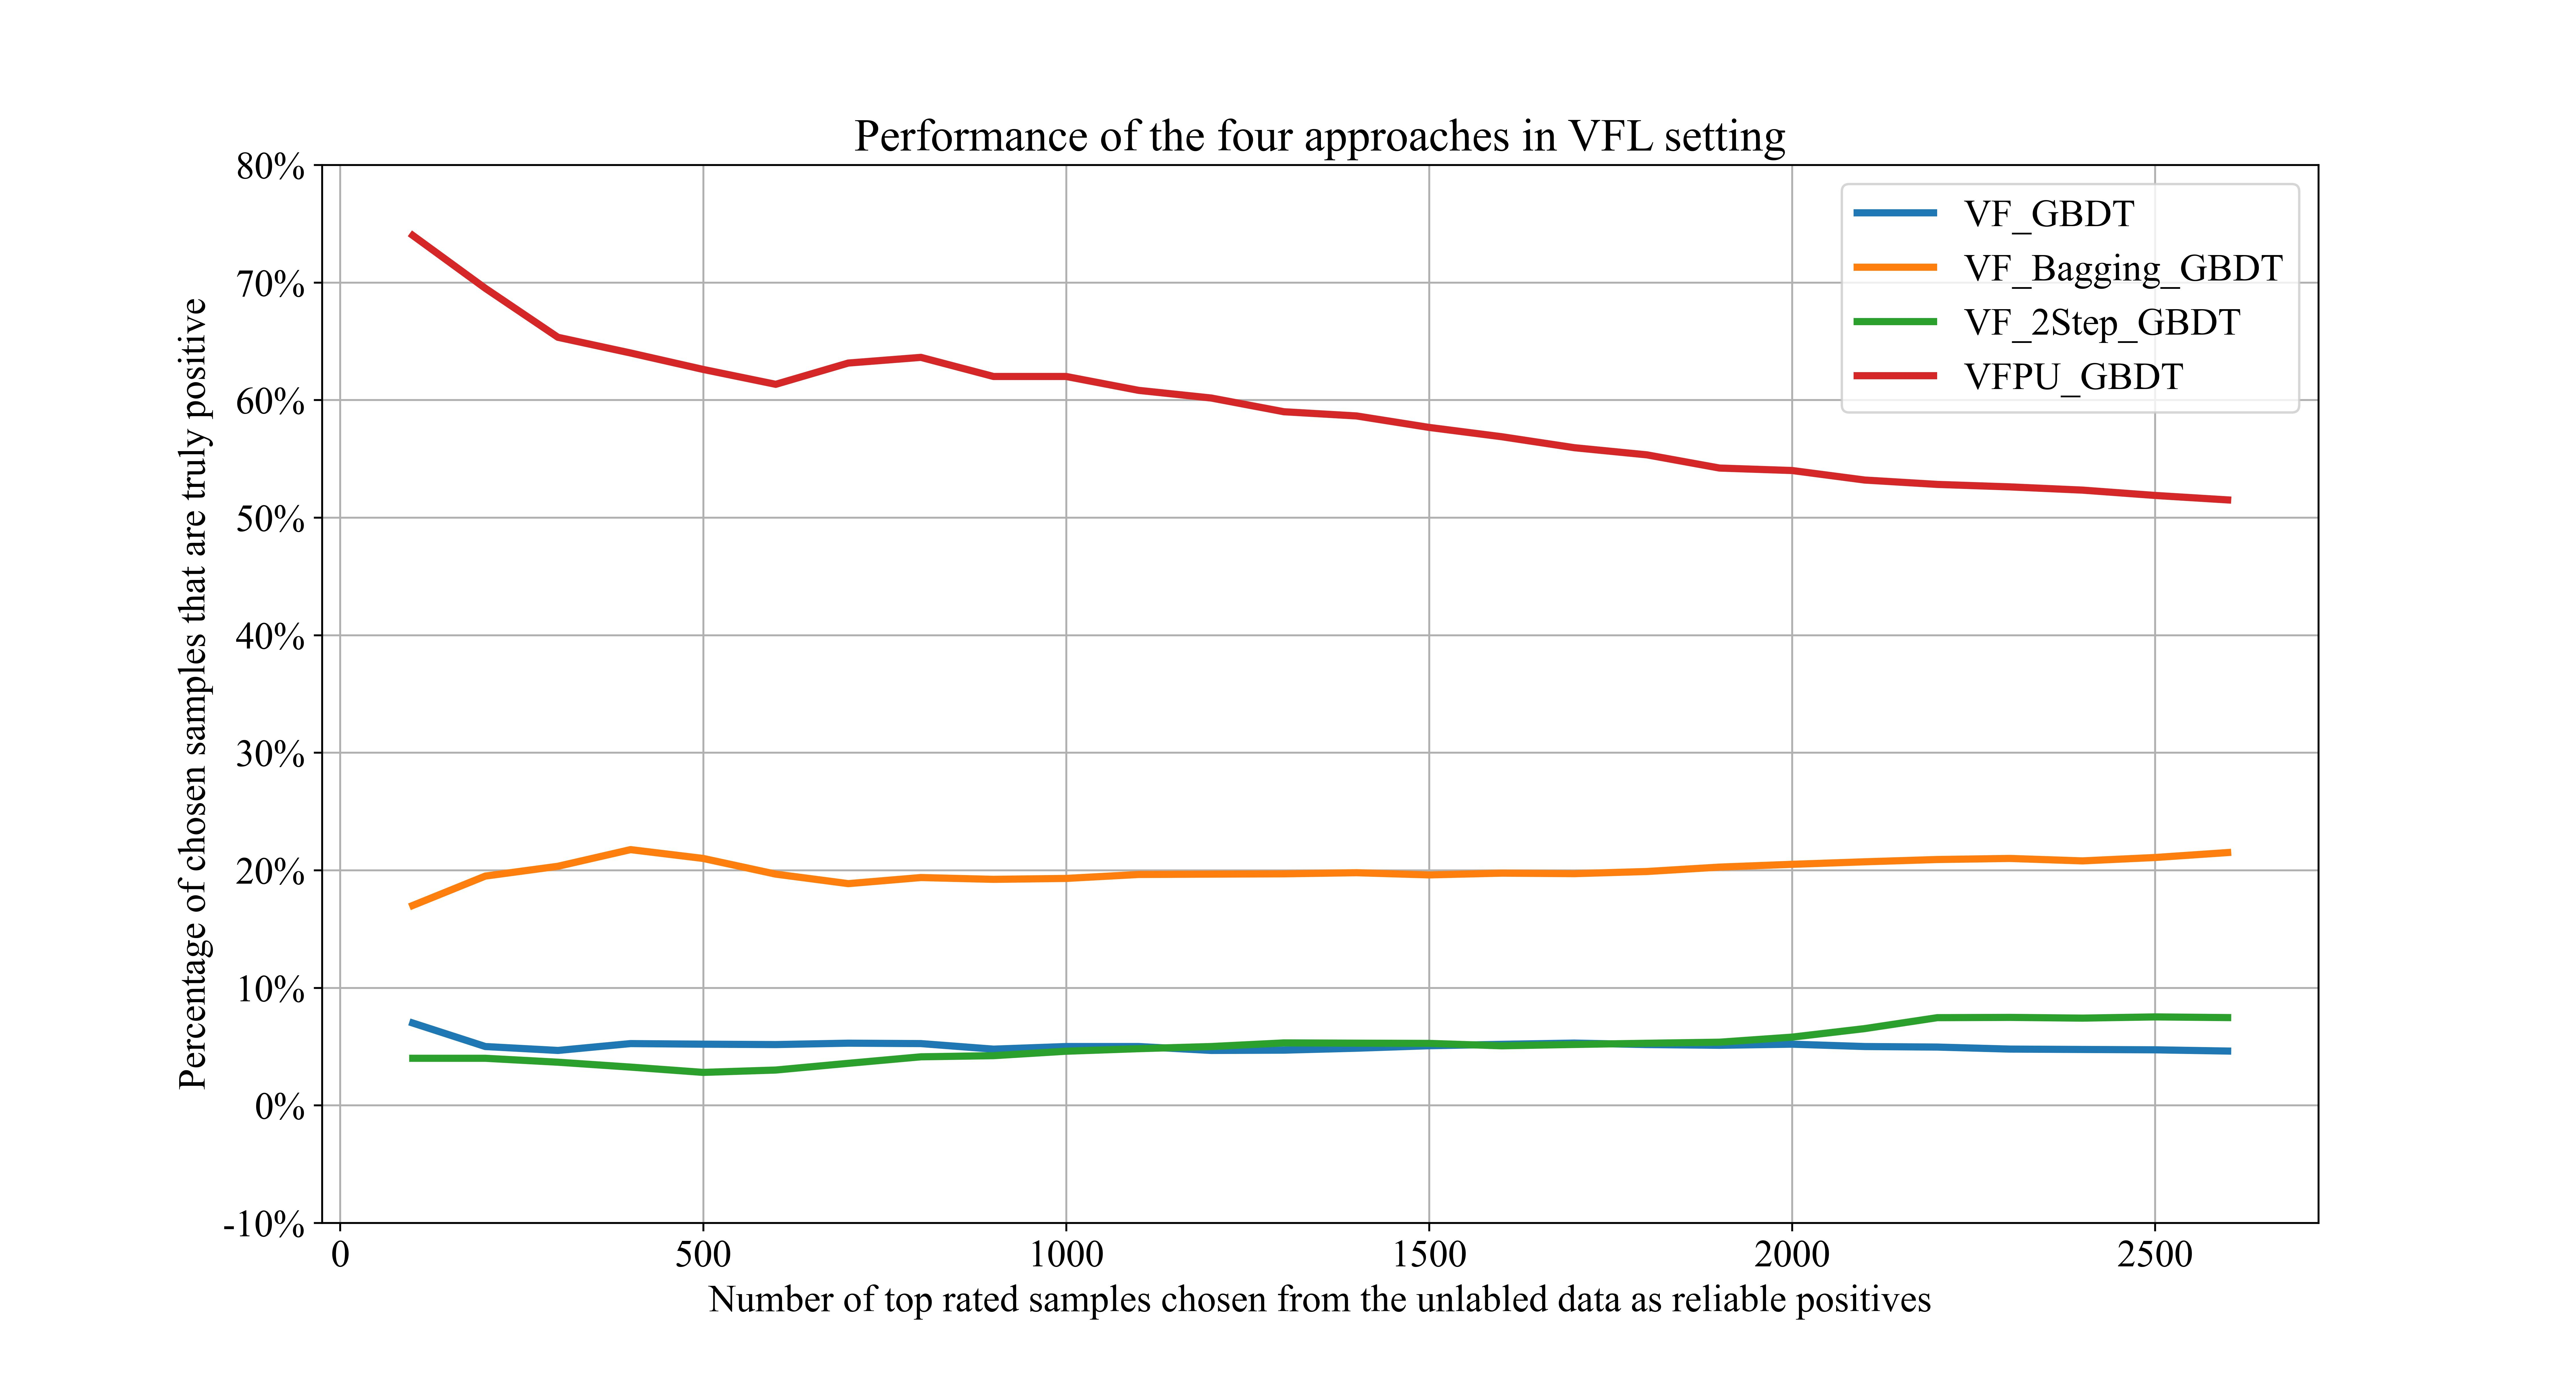
\includegraphics[width=0.9\textwidth,height=9cm]{chapters/imgs/Figure 5 in JPEG format}
    \bicaption[\xiaosi 在纵向联邦学习中通过不同的半监督方法获得的准确推荐百分比]{\wuhao 在纵向联邦学习中通过不同的半监督方法获得的准确推荐百分比(Bank数据集)}{\wuhao The accurate recommendations percentage by Different Semi-supervised Methods in VFL (The Bank Marketing Dataset)}
	\label{fig:GBDT}
\end{figure}











\begin{figure}[!htbp]  % 开始一个浮动图形环境,位置指定符:!htbp(此处、顶部、底部、单独页面)
    \centering  % 使图形居中对齐
    \vspace{0.5cm} % 调整图片与上文的间距,增加0.5厘米的垂直空间
    \captionsetup{size=footnotesize}  % 设置标题字体大小为脚注大小
    
    % 创建第一个子图(a),设置标签为RQ2.1.sub1,插入图片,宽度为0.45倍文本宽度,高度为5.1厘米
    \subfigure[]{\label{RQ2.1.sub1}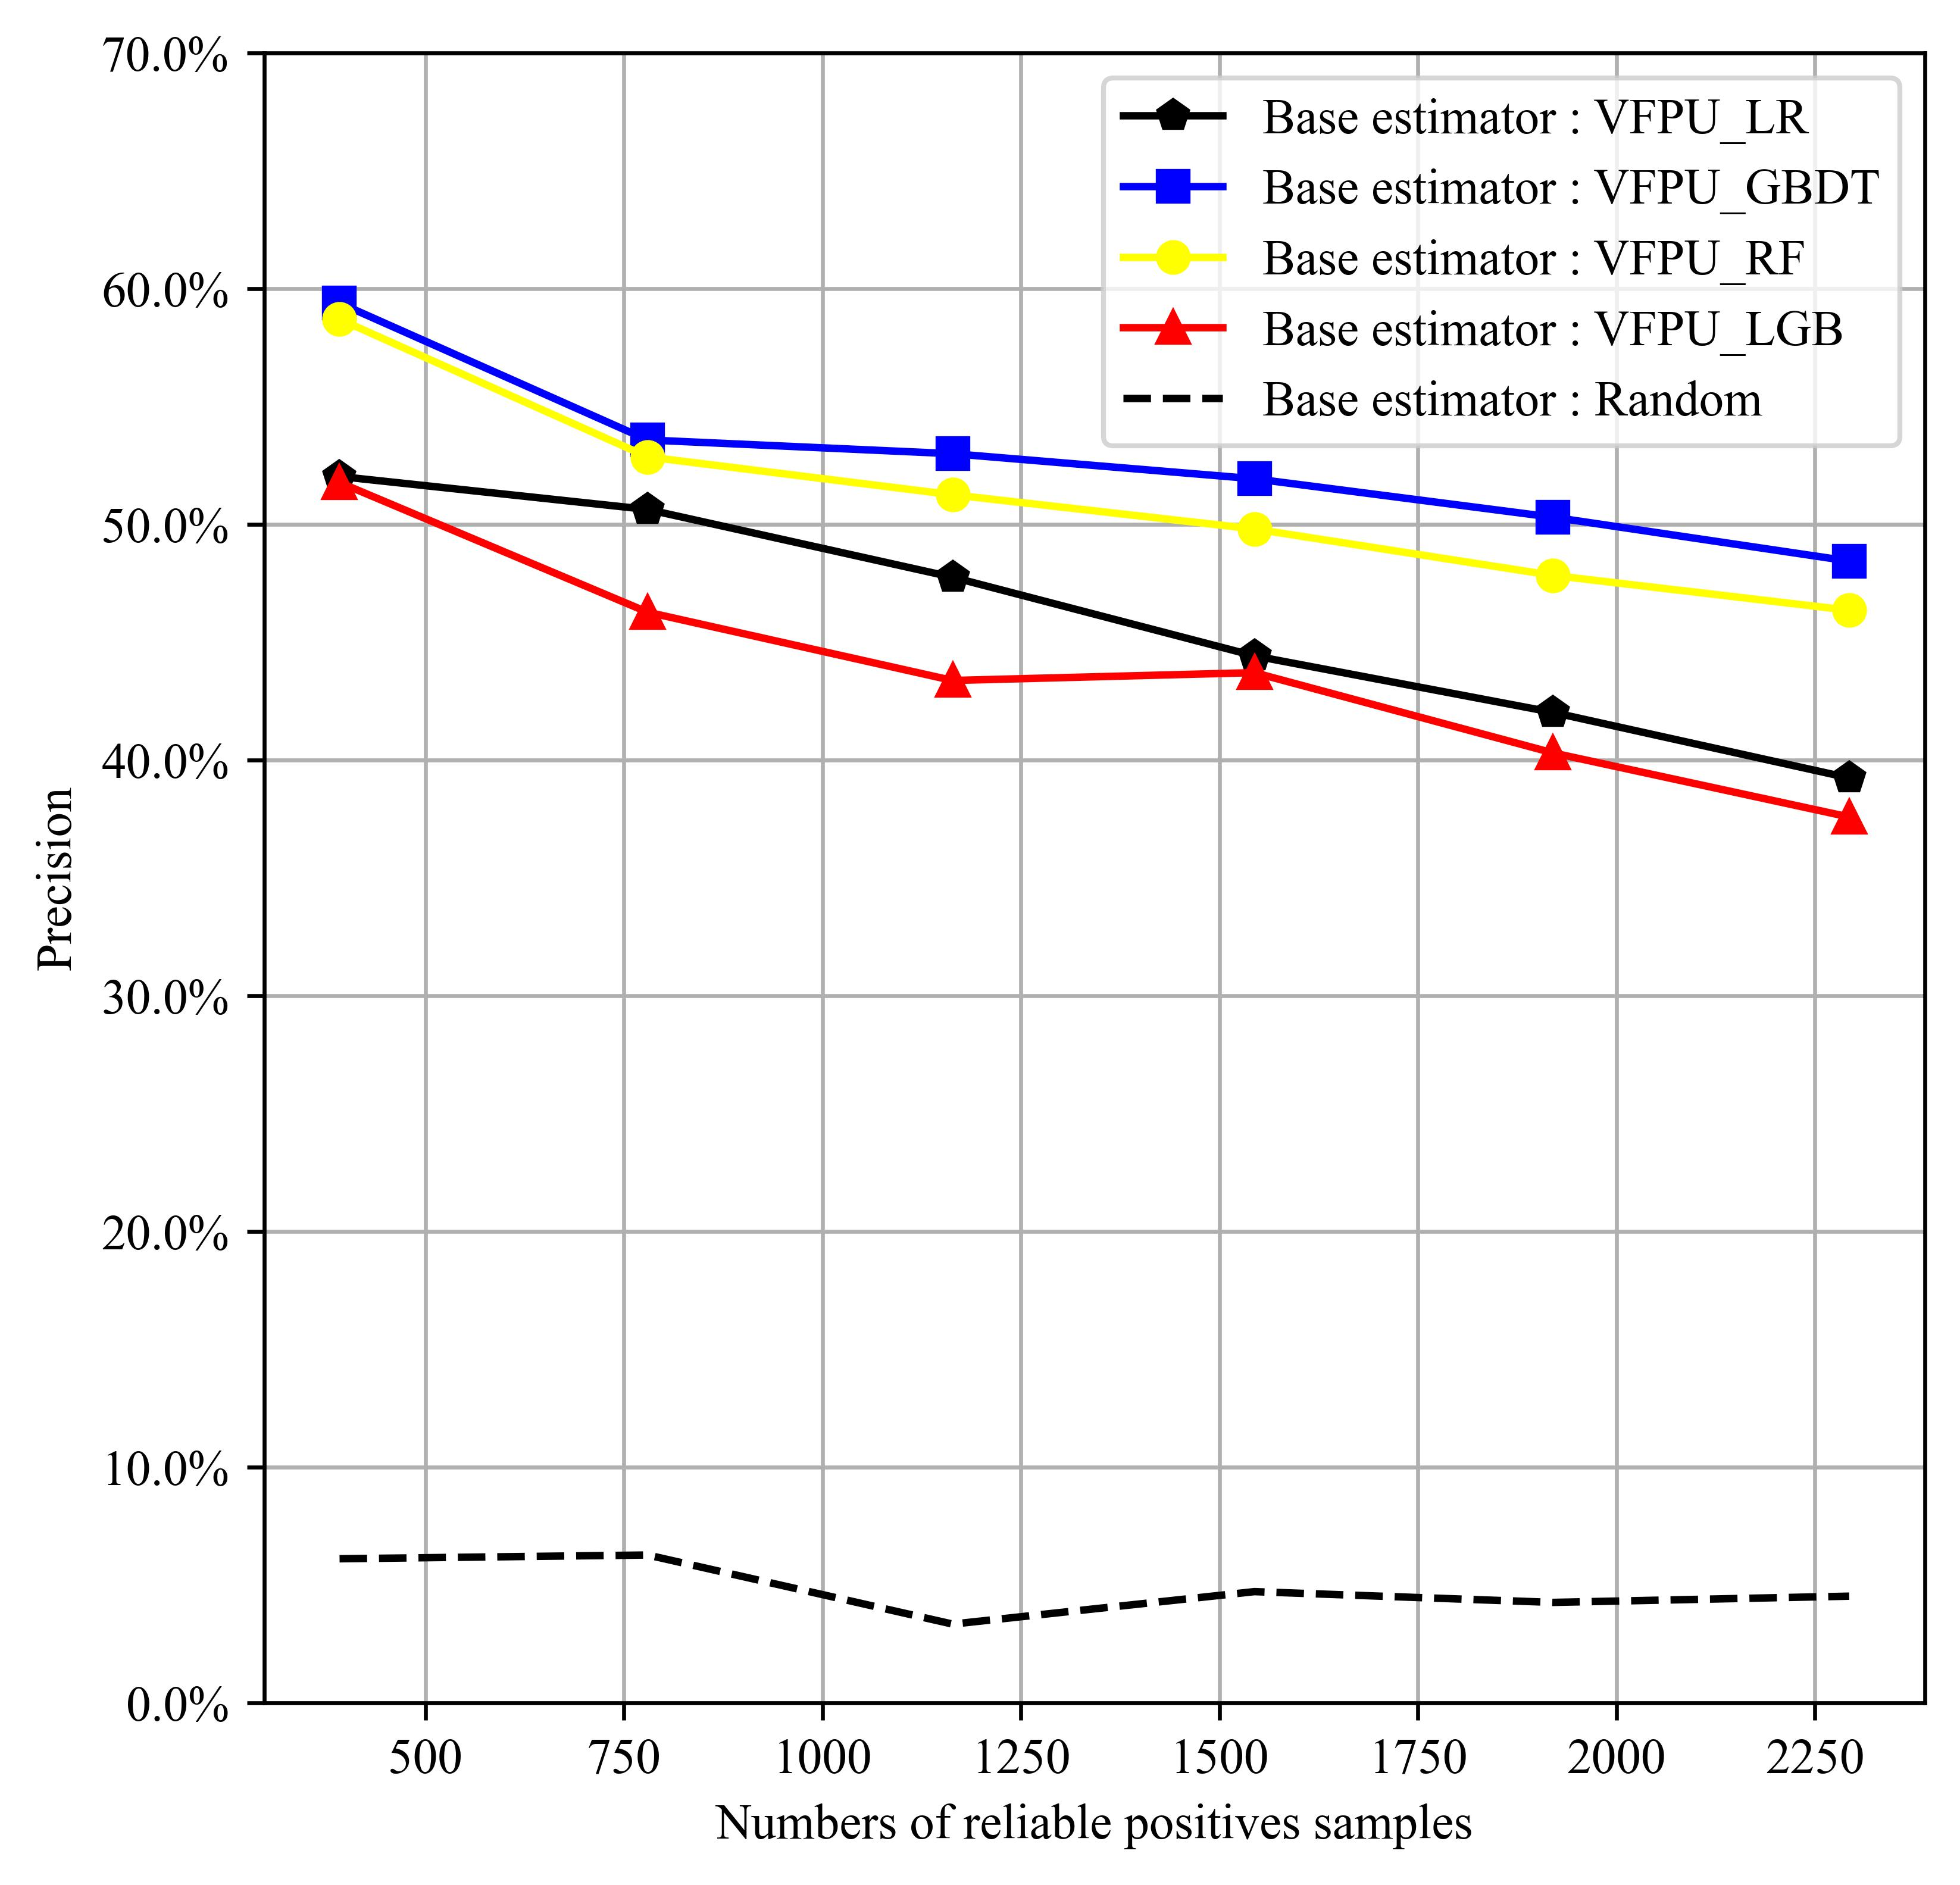
\includegraphics[width=0.45\textwidth,height=5.1cm]{chapters/imgs/Figure 2 (1) in JEPG format}}
    
    % 创建第二个子图(b),设置标签为RQ2.1.sub2,插入图片,宽度为0.45倍文本宽度,高度为5.1厘米
    \subfigure[]{\label{RQ2.1.sub2}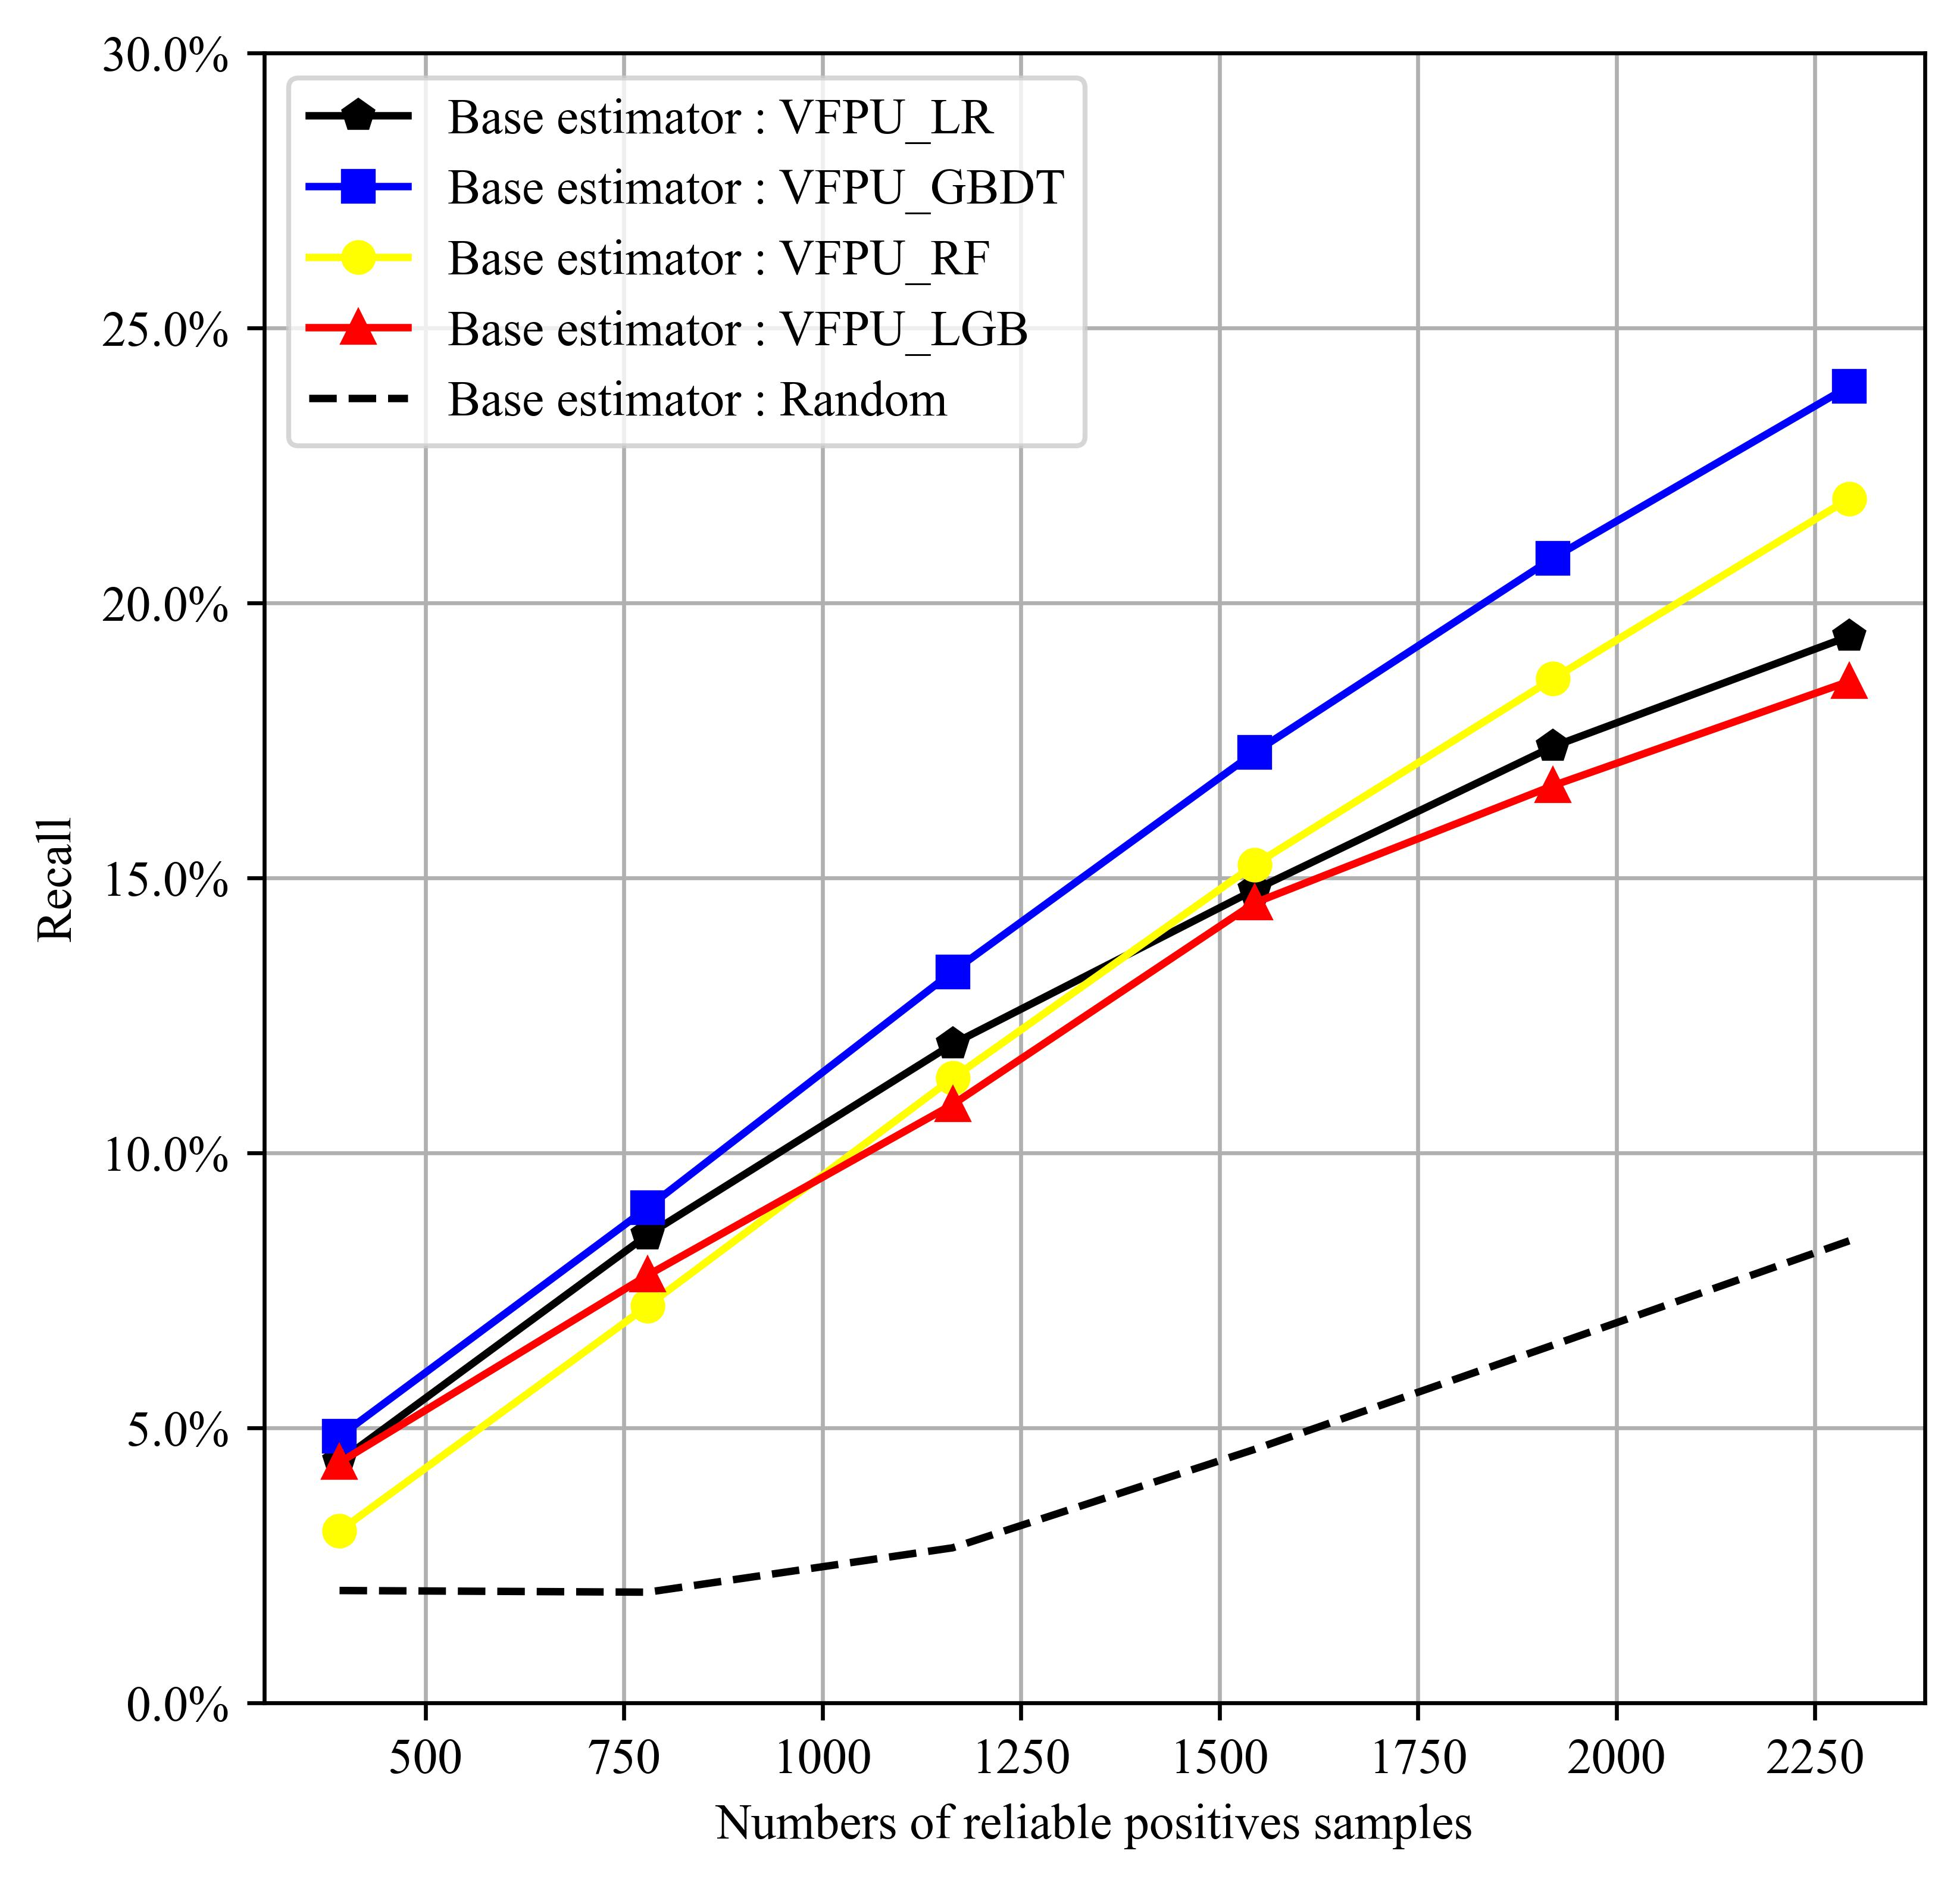
\includegraphics[width=0.45\textwidth,height=5.1cm]{chapters/imgs/Figure 2 (2) in JEPG format}}
    
    % 创建第三个子图(c),设置标签为RQ2.1.sub3,插入图片,宽度为0.45倍文本宽度,高度为5.1厘米
    \subfigure[]{\label{RQ2.1.sub3}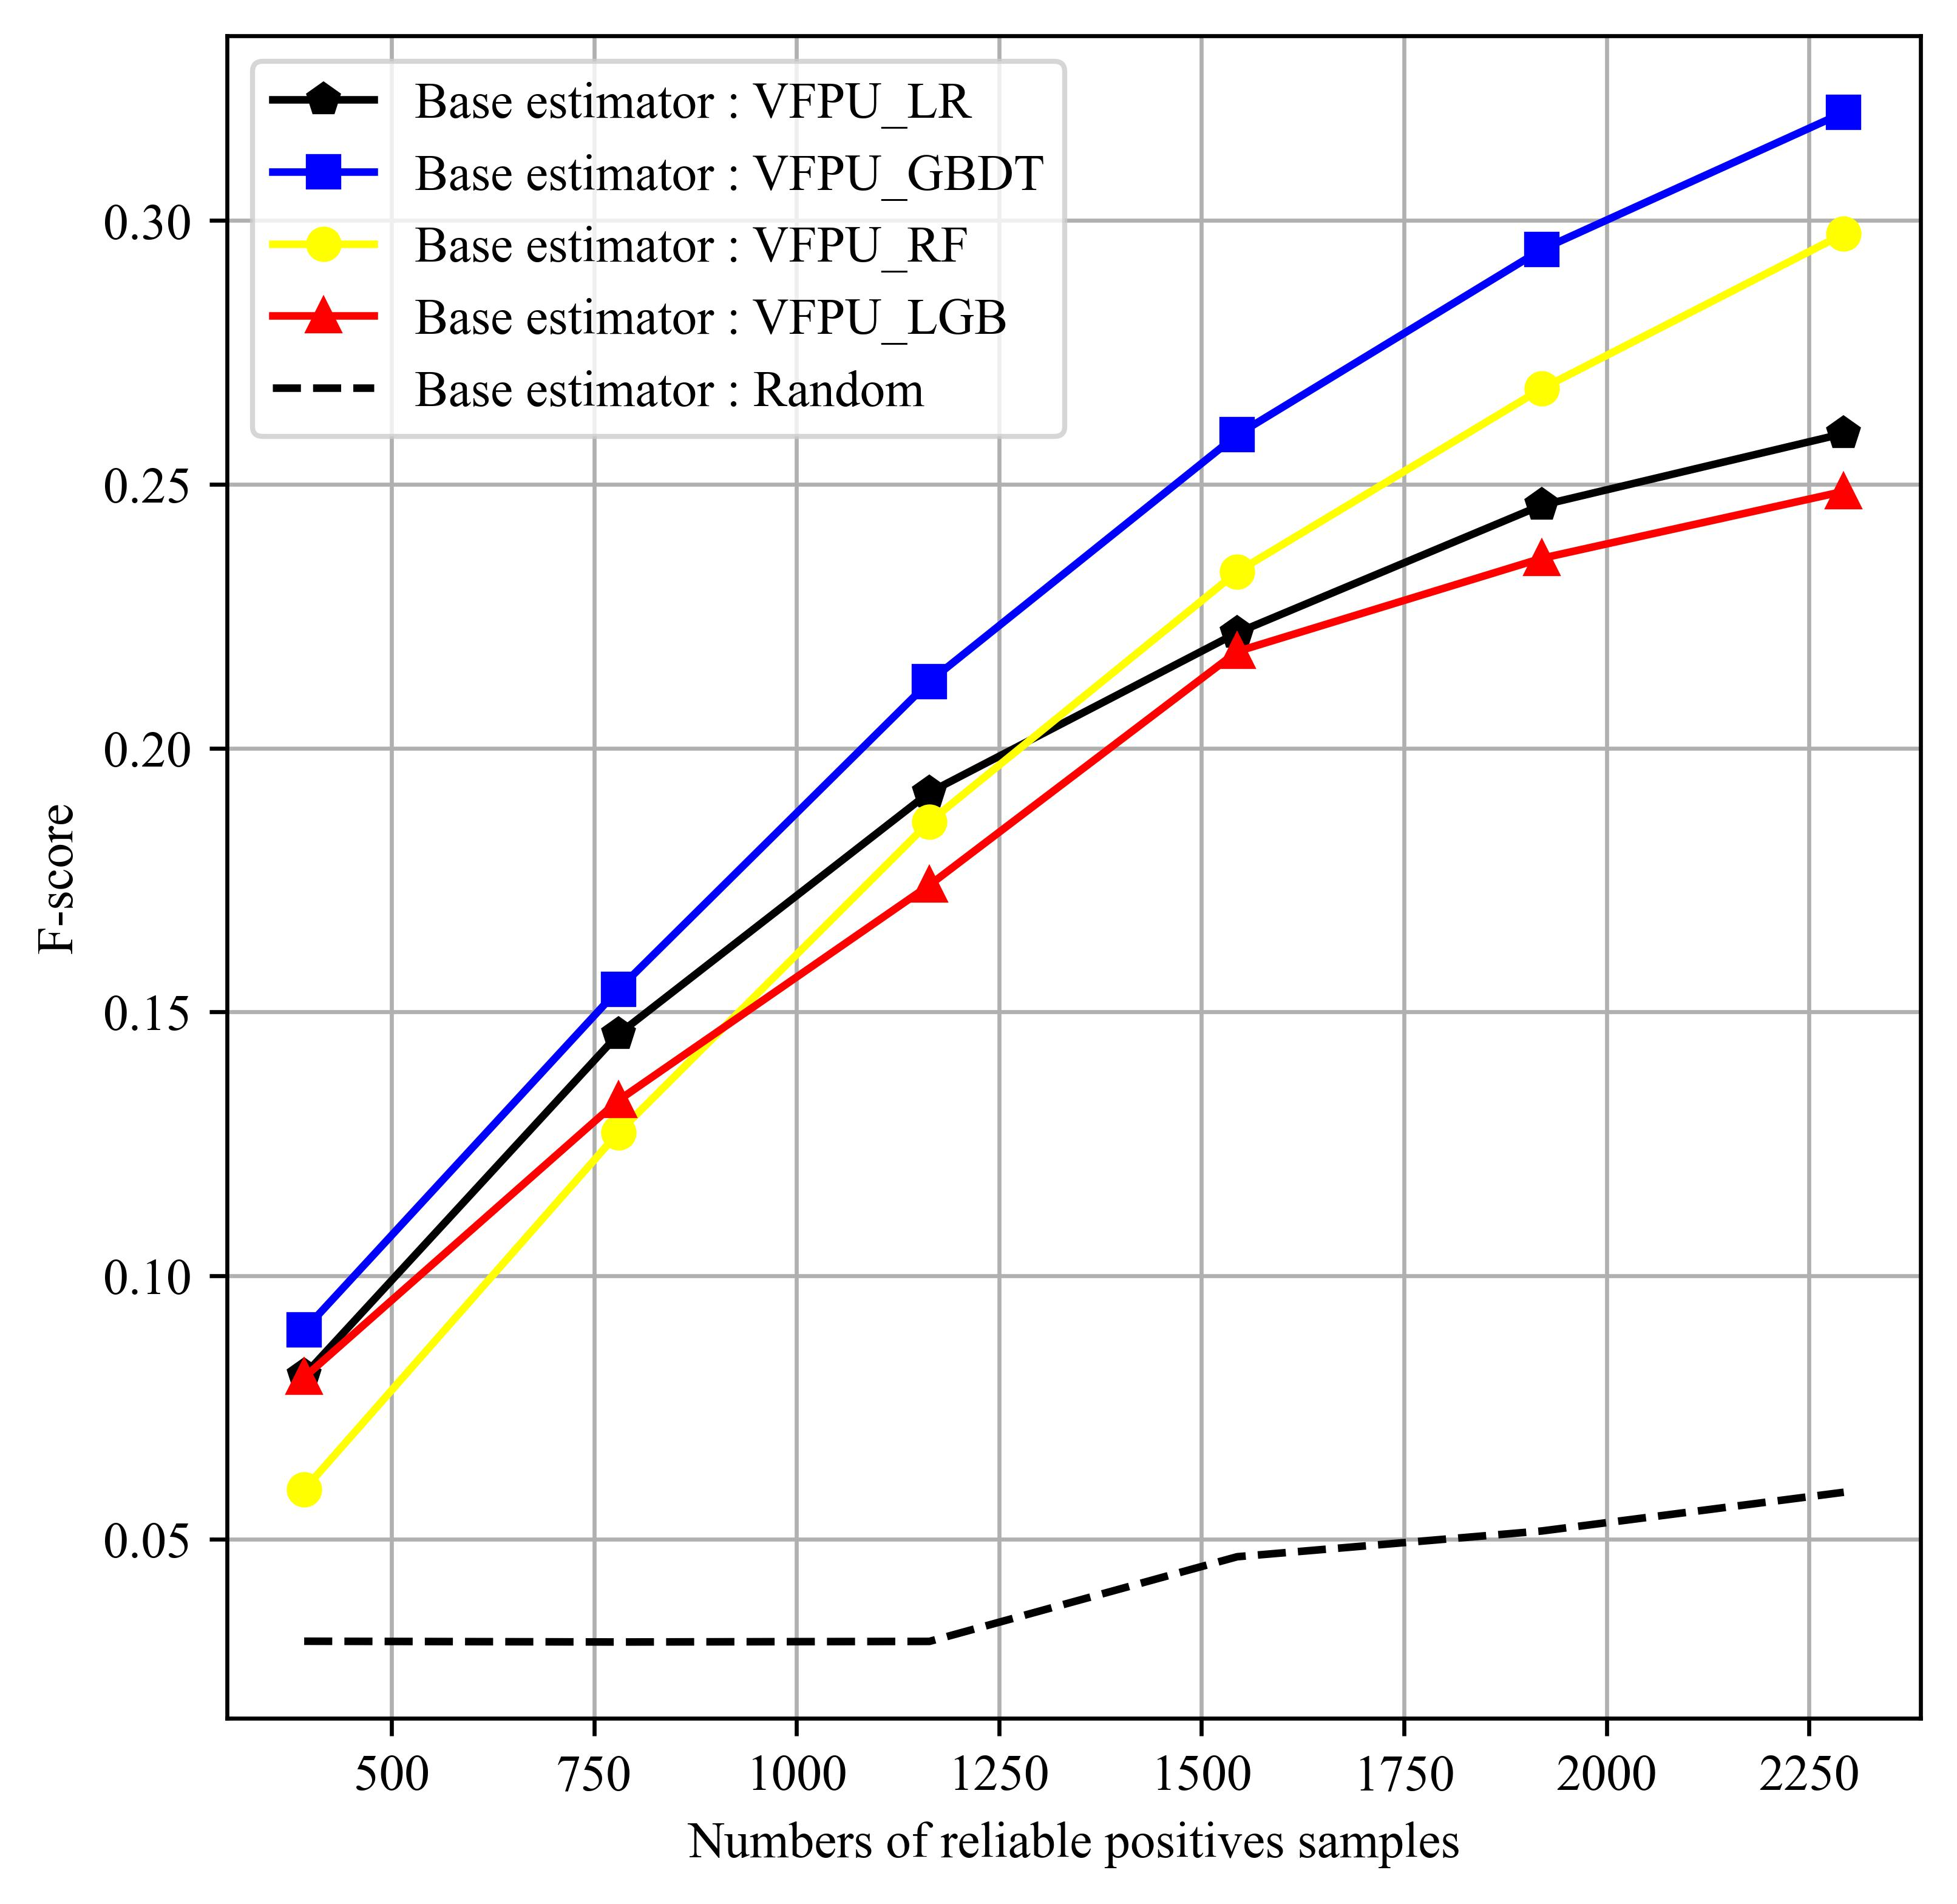
\includegraphics[width=0.45\textwidth,height=5.1cm]{chapters/imgs/Figure 2 (3) in JEPG format}}
    
    % 创建第四个子图(d),设置标签为RQ2.1.sub4,插入图片,宽度为0.45倍文本宽度,高度为5.1厘米
    \subfigure[]{\label{RQ2.1.sub4}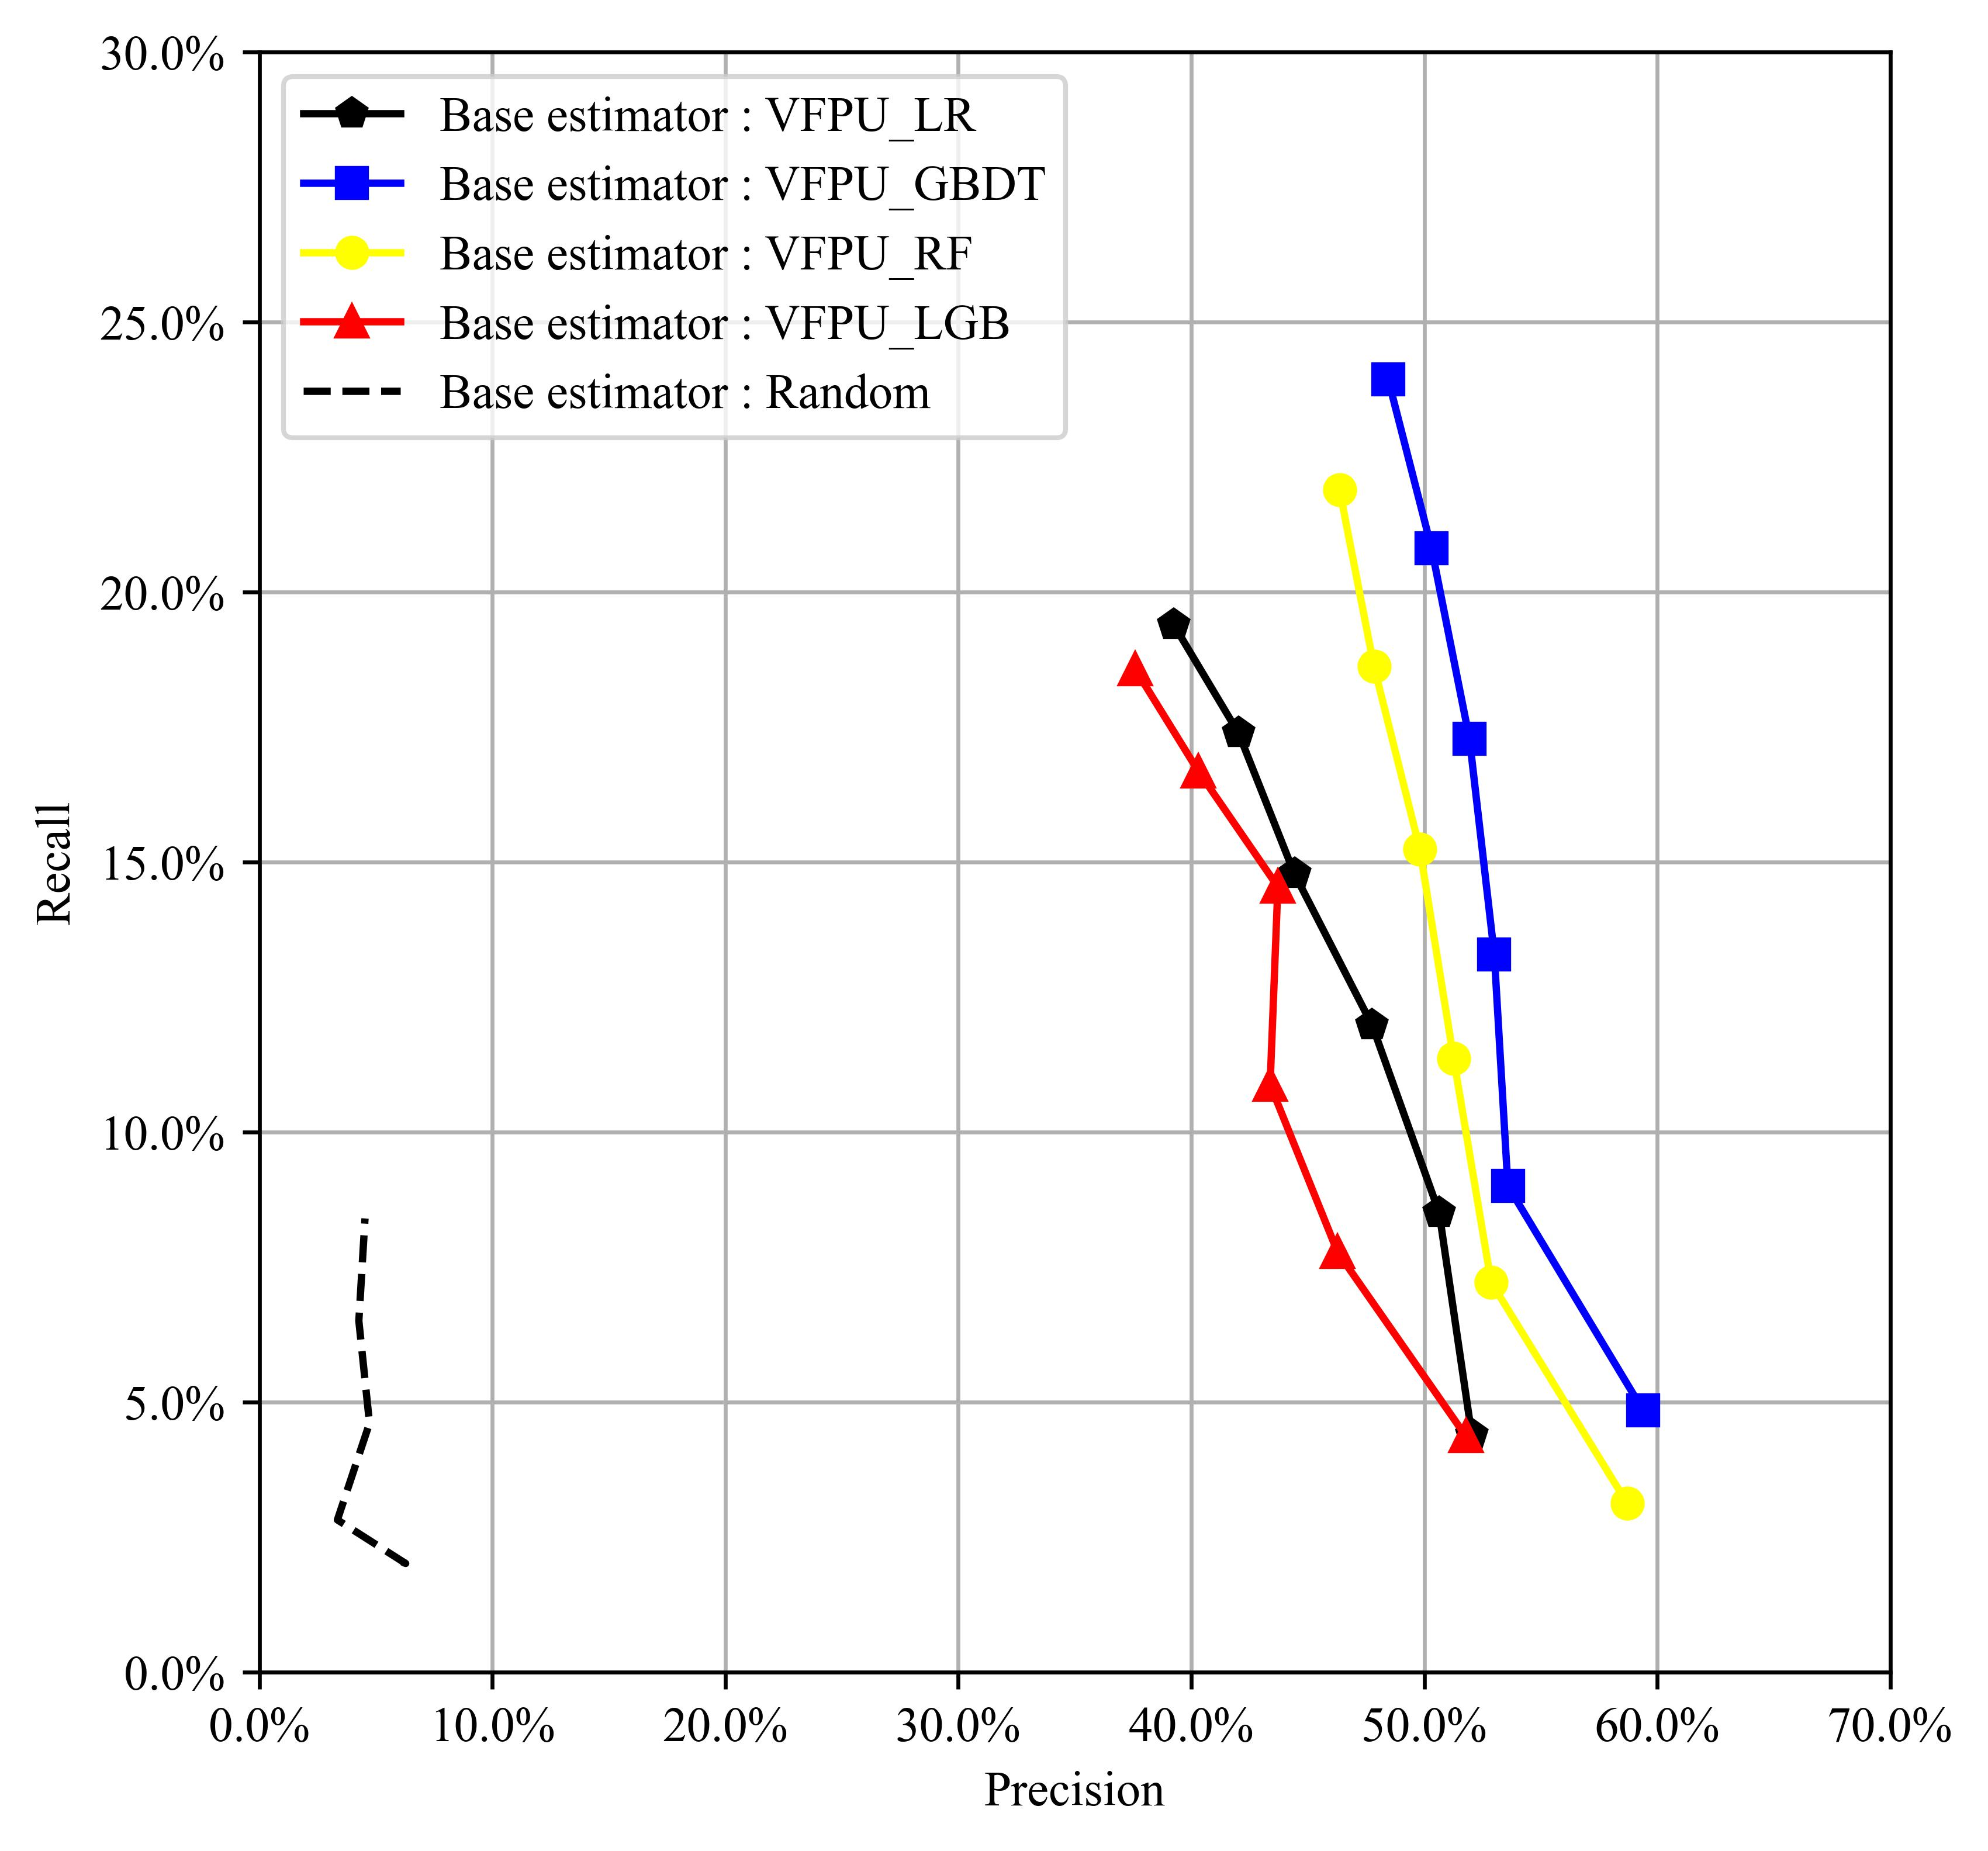
\includegraphics[width=0.45\textwidth,height=5.1cm]{chapters/imgs/Figure 2 (4) in JEPG format}}
    
    % 开始一个带有特定边距的项目列表环境
    \begin{itemize}[leftmargin=1.6cm,rightmargin=1.6cm]
        % 使用自定义项目符号(空白)创建一个项目,包含双语标题
        \item[\quad] \bicaption
            % 中文标题的短版本(用于目录),使用小四号字体
            [\xiaosi 不同基学器在不同可靠正样本数量下的性能]
            % 中文标题的完整版本,使用宋体五号字体,居中对齐
            {\centering \songti \wuhao 不同基学器在不同可靠正样本数量下的性能:(a)精度;(b)召回率;(c)F-score;(d)精度-召回率(Bank 数据集)}
            % 英文标题,使用五号字体,居中对齐
            {\centering \wuhao Performance of Different Base Estimators with Varying Reliable Positive Samples: (a) Precision; (b) Recall; (c) F-score; (d) Precision-Recall (The Bank Marketing Dataset)}
    \end{itemize}
    
    \label{RQ2.1}  % 为整个图形设置标签RQ2.1,可用于交叉引用
\end{figure}  % 结束图形环境







\begin{figure}[!htbp]
	\centering
	\vspace{0.5cm} % 调整图片与上文的间距
	\captionsetup{size=footnotesize}
	
	\subfigure[]{\label{RQ2.1.sub1}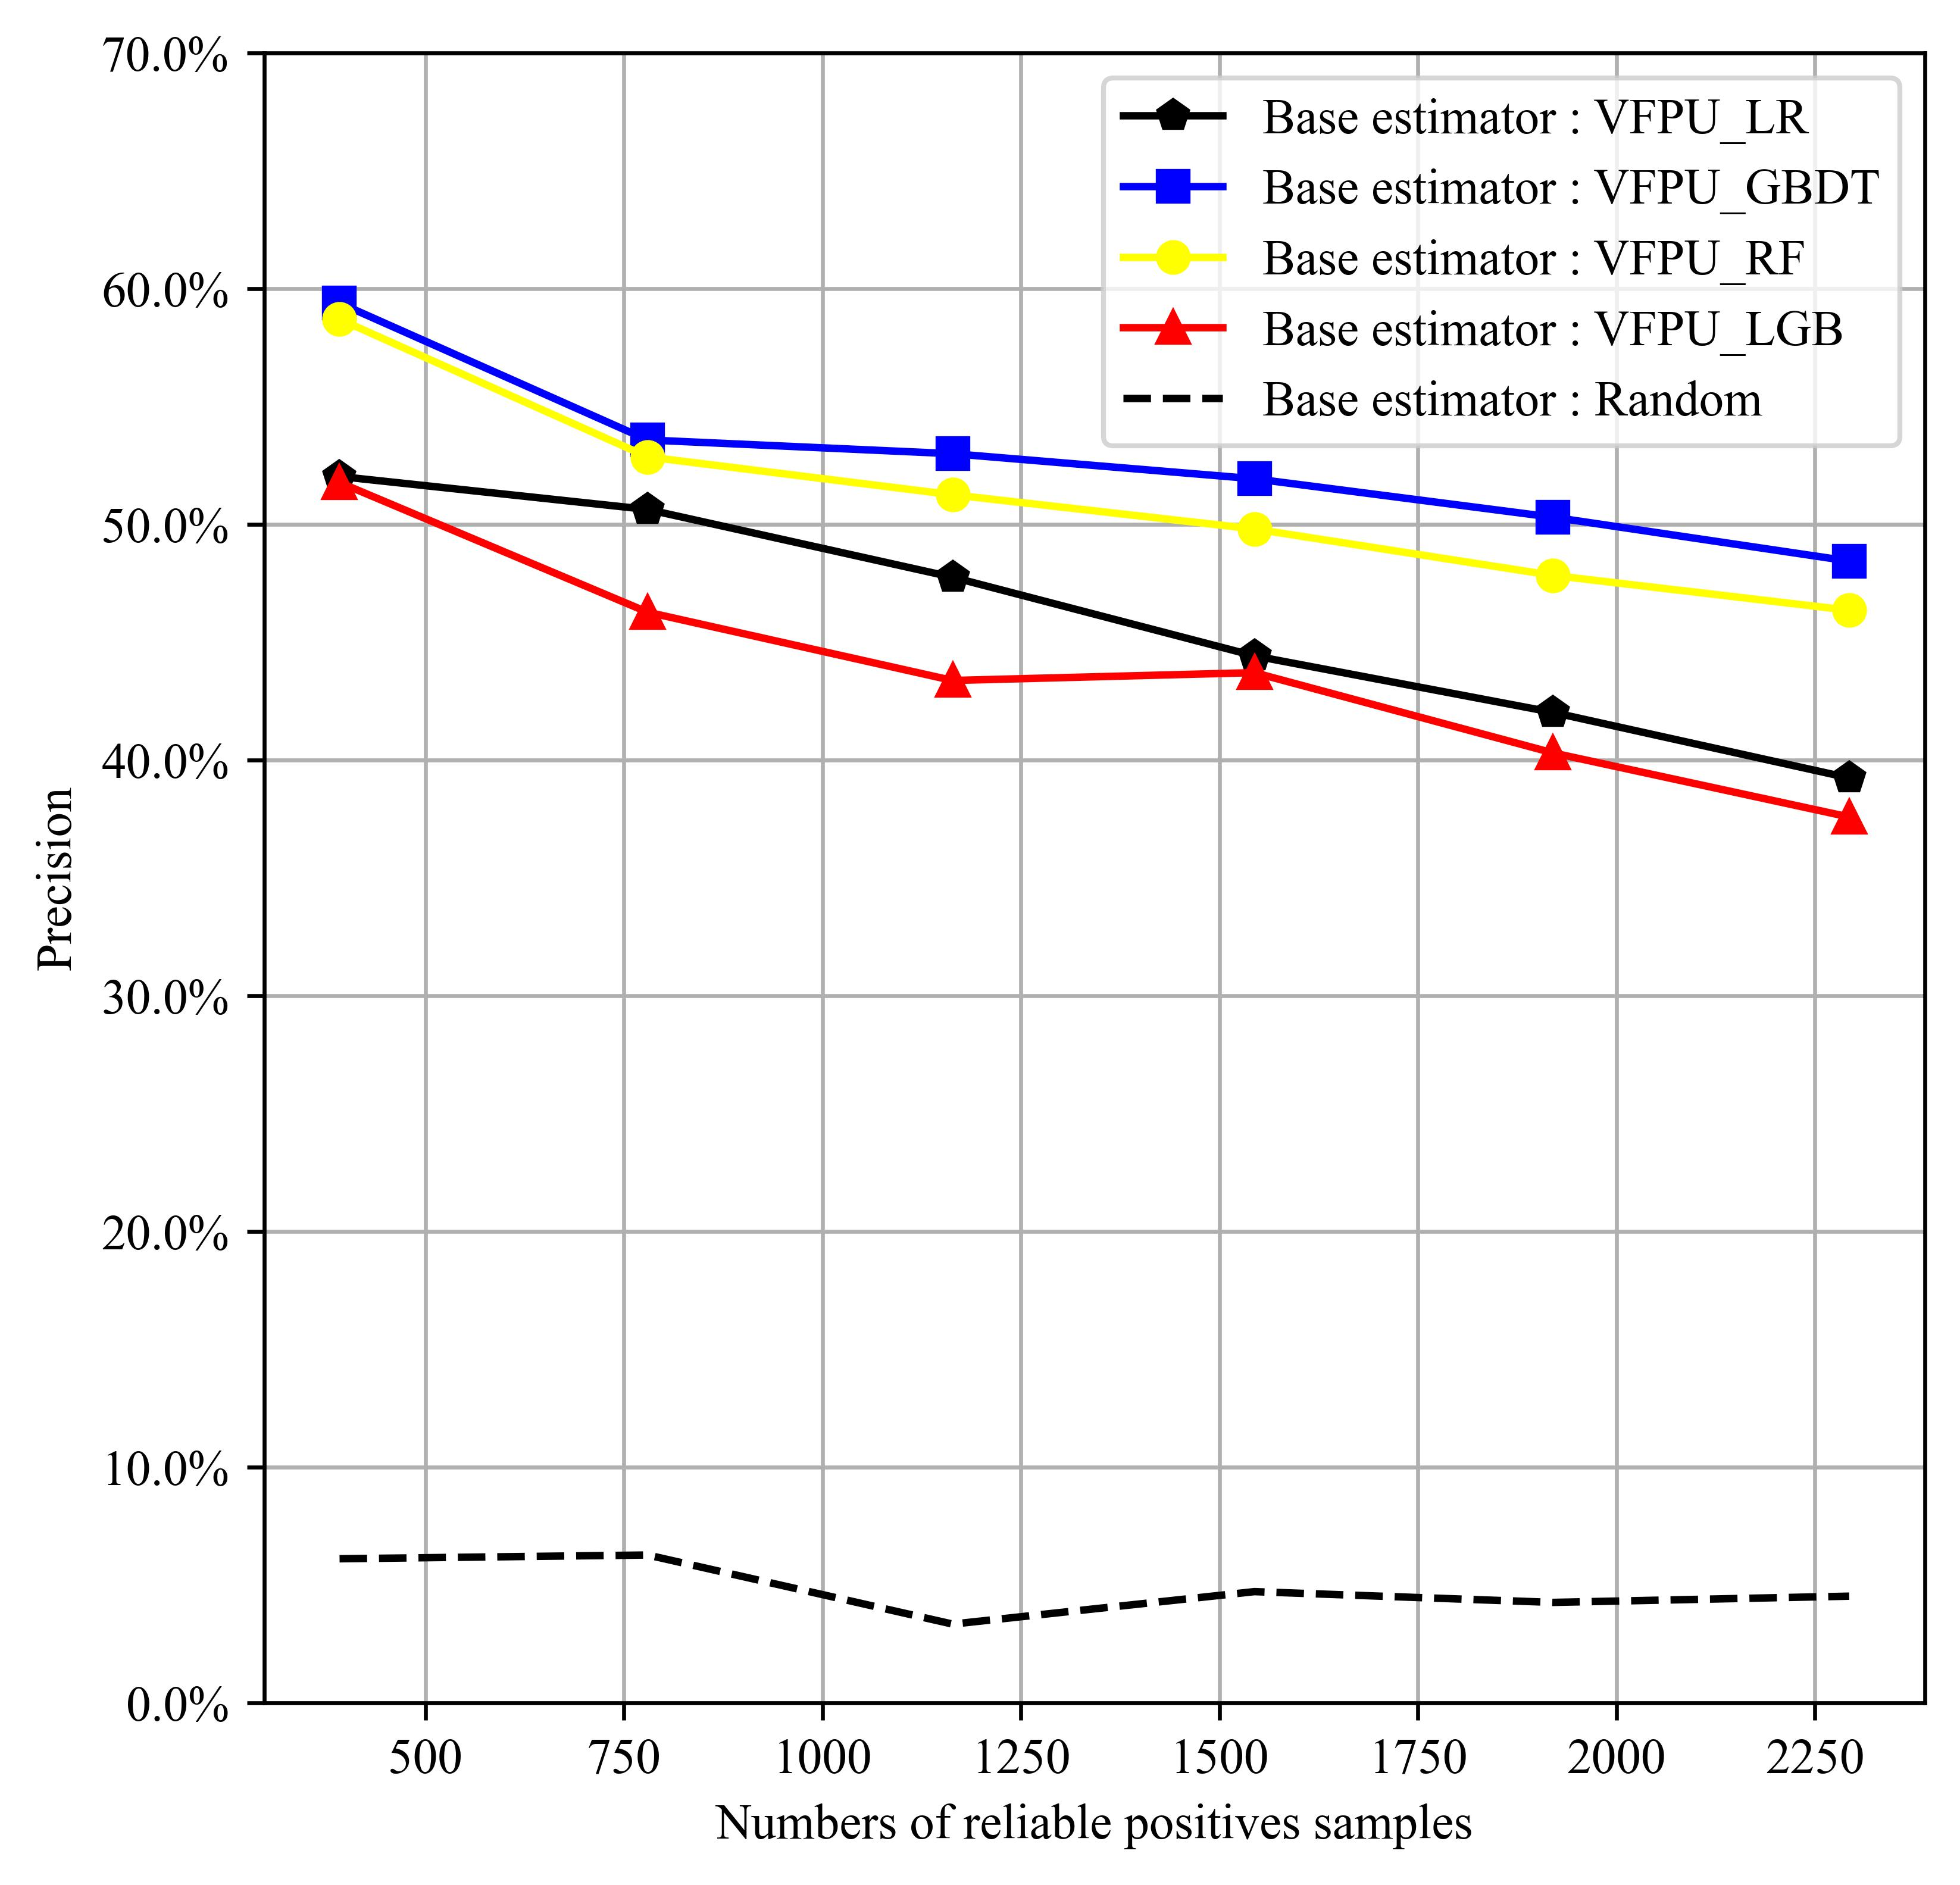
\includegraphics[width=0.45\textwidth,height=5.1cm]{chapters/imgs/Figure 2 (1) in JEPG format}}
	\subfigure[]{\label{RQ2.1.sub2}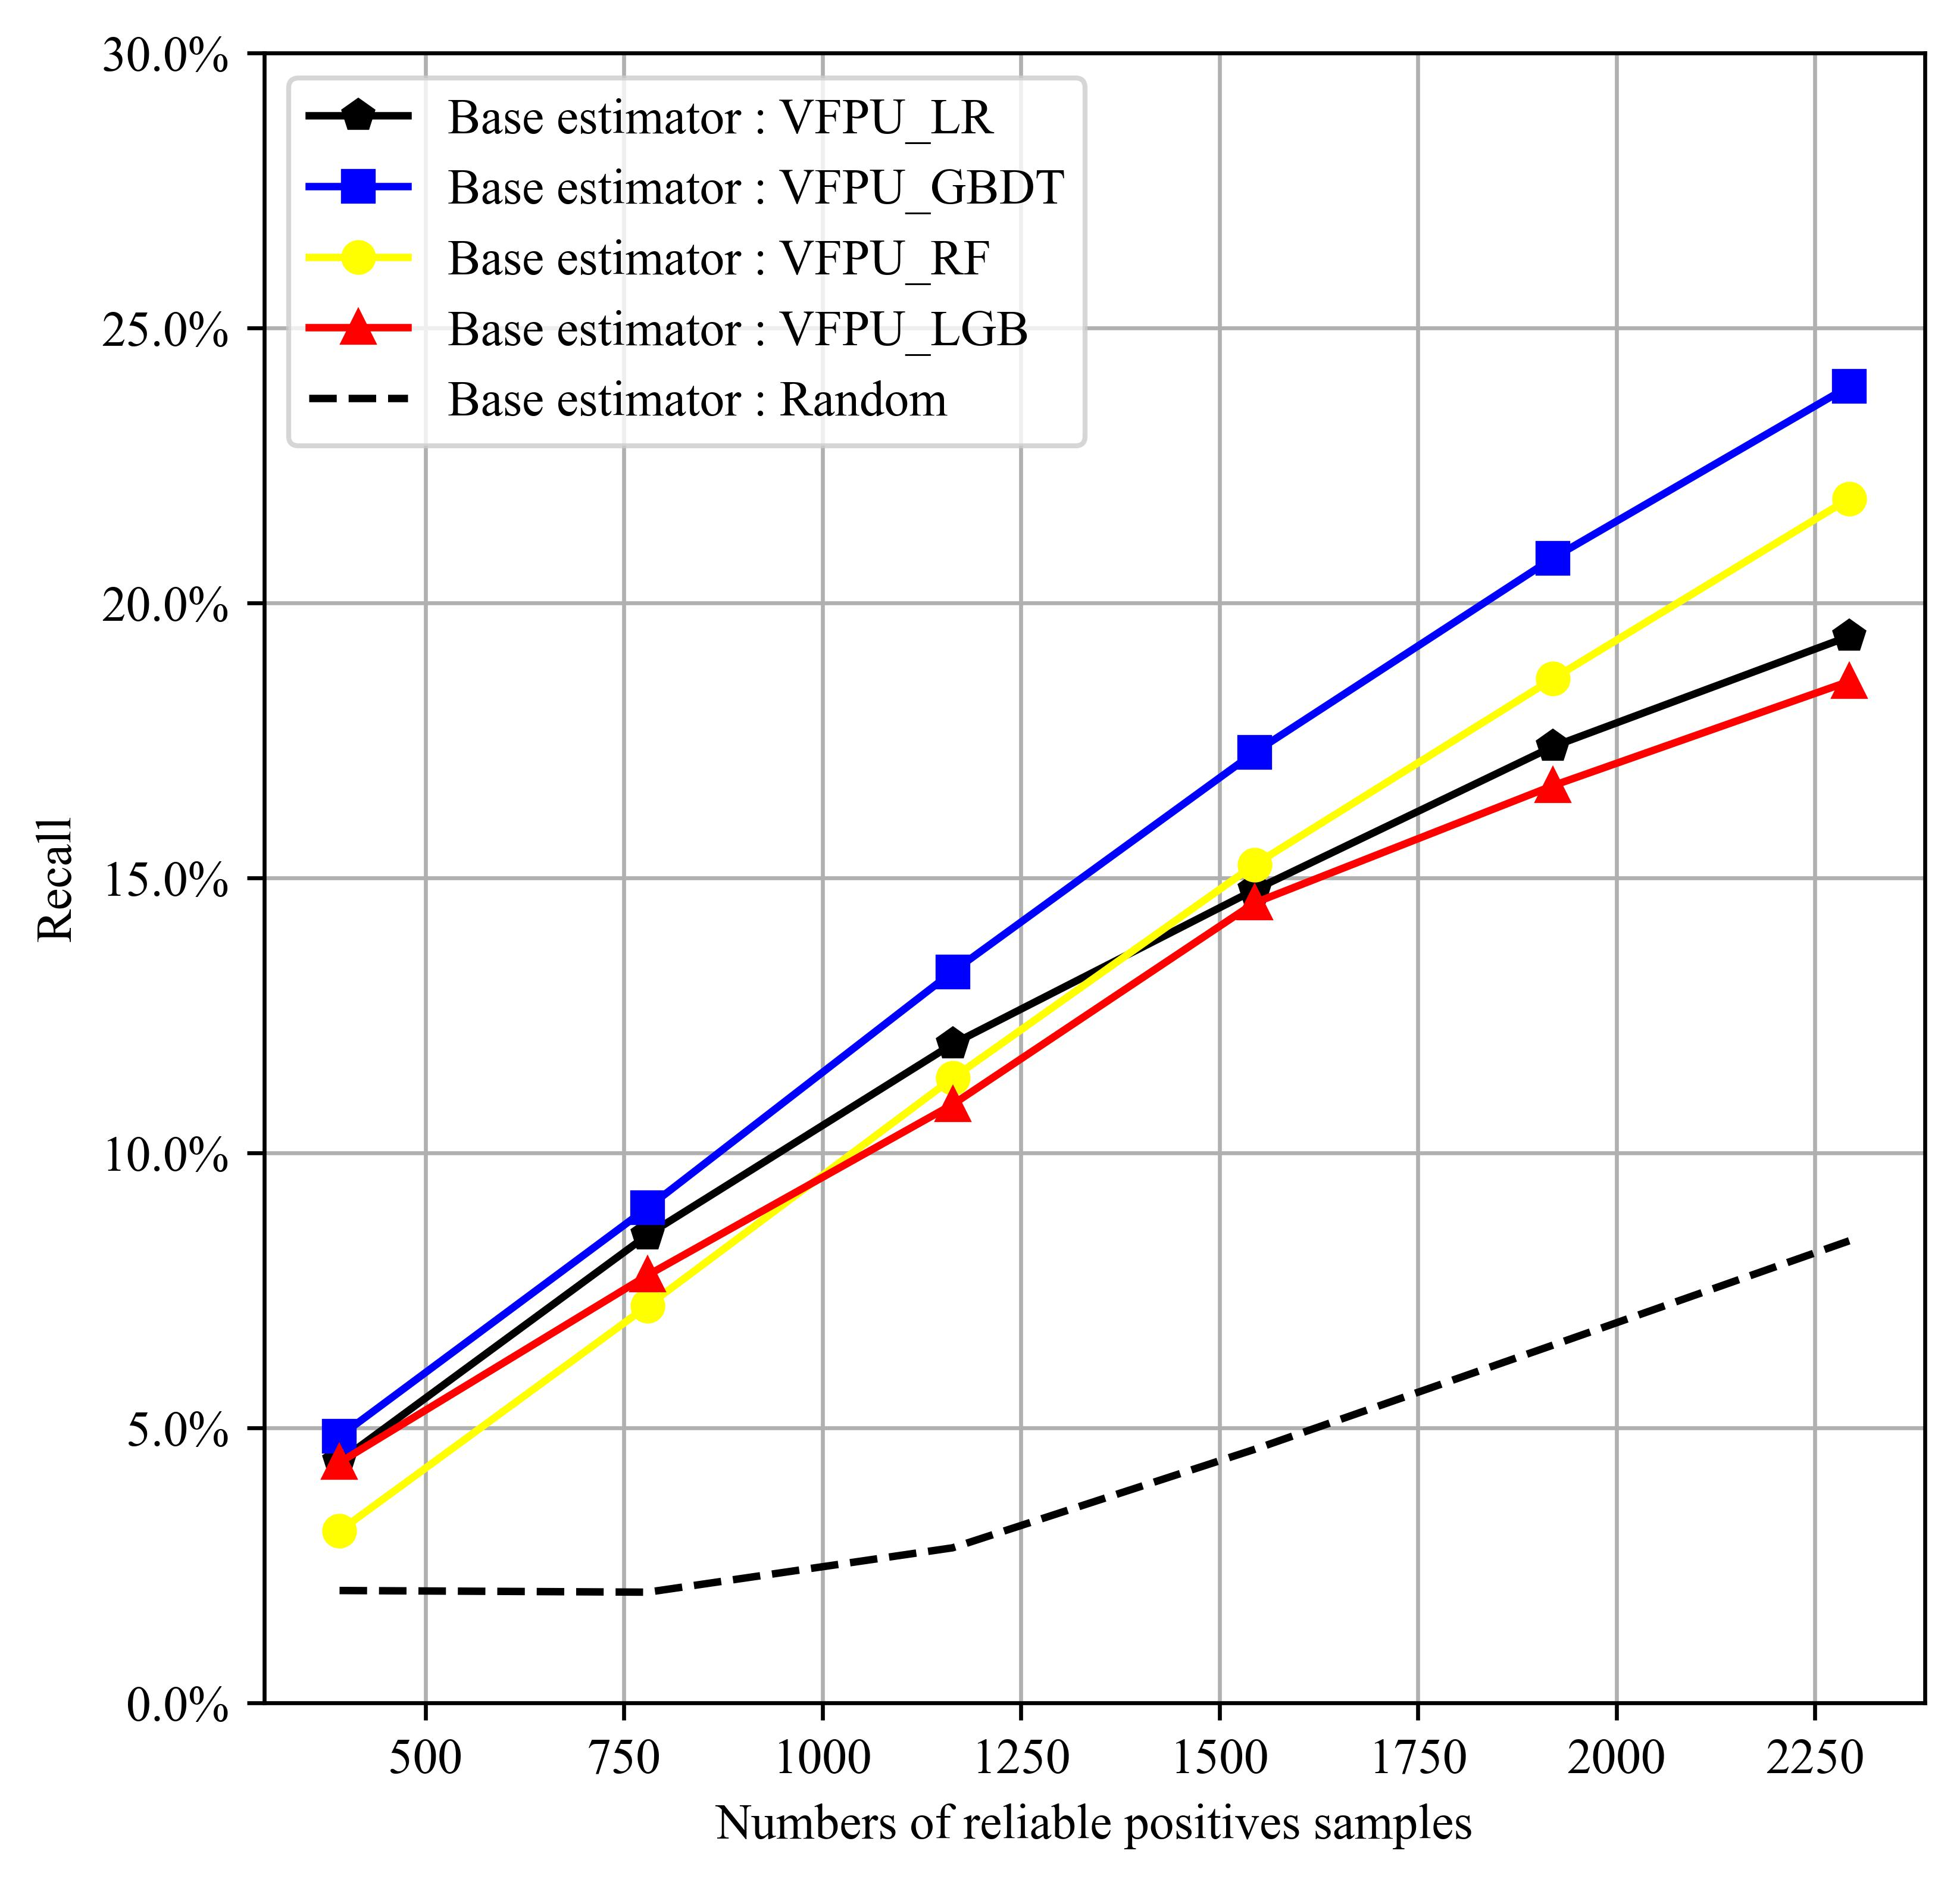
\includegraphics[width=0.45\textwidth,height=5.1cm]{chapters/imgs/Figure 2 (2) in JEPG format}}
	\subfigure[]{\label{RQ2.1.sub3}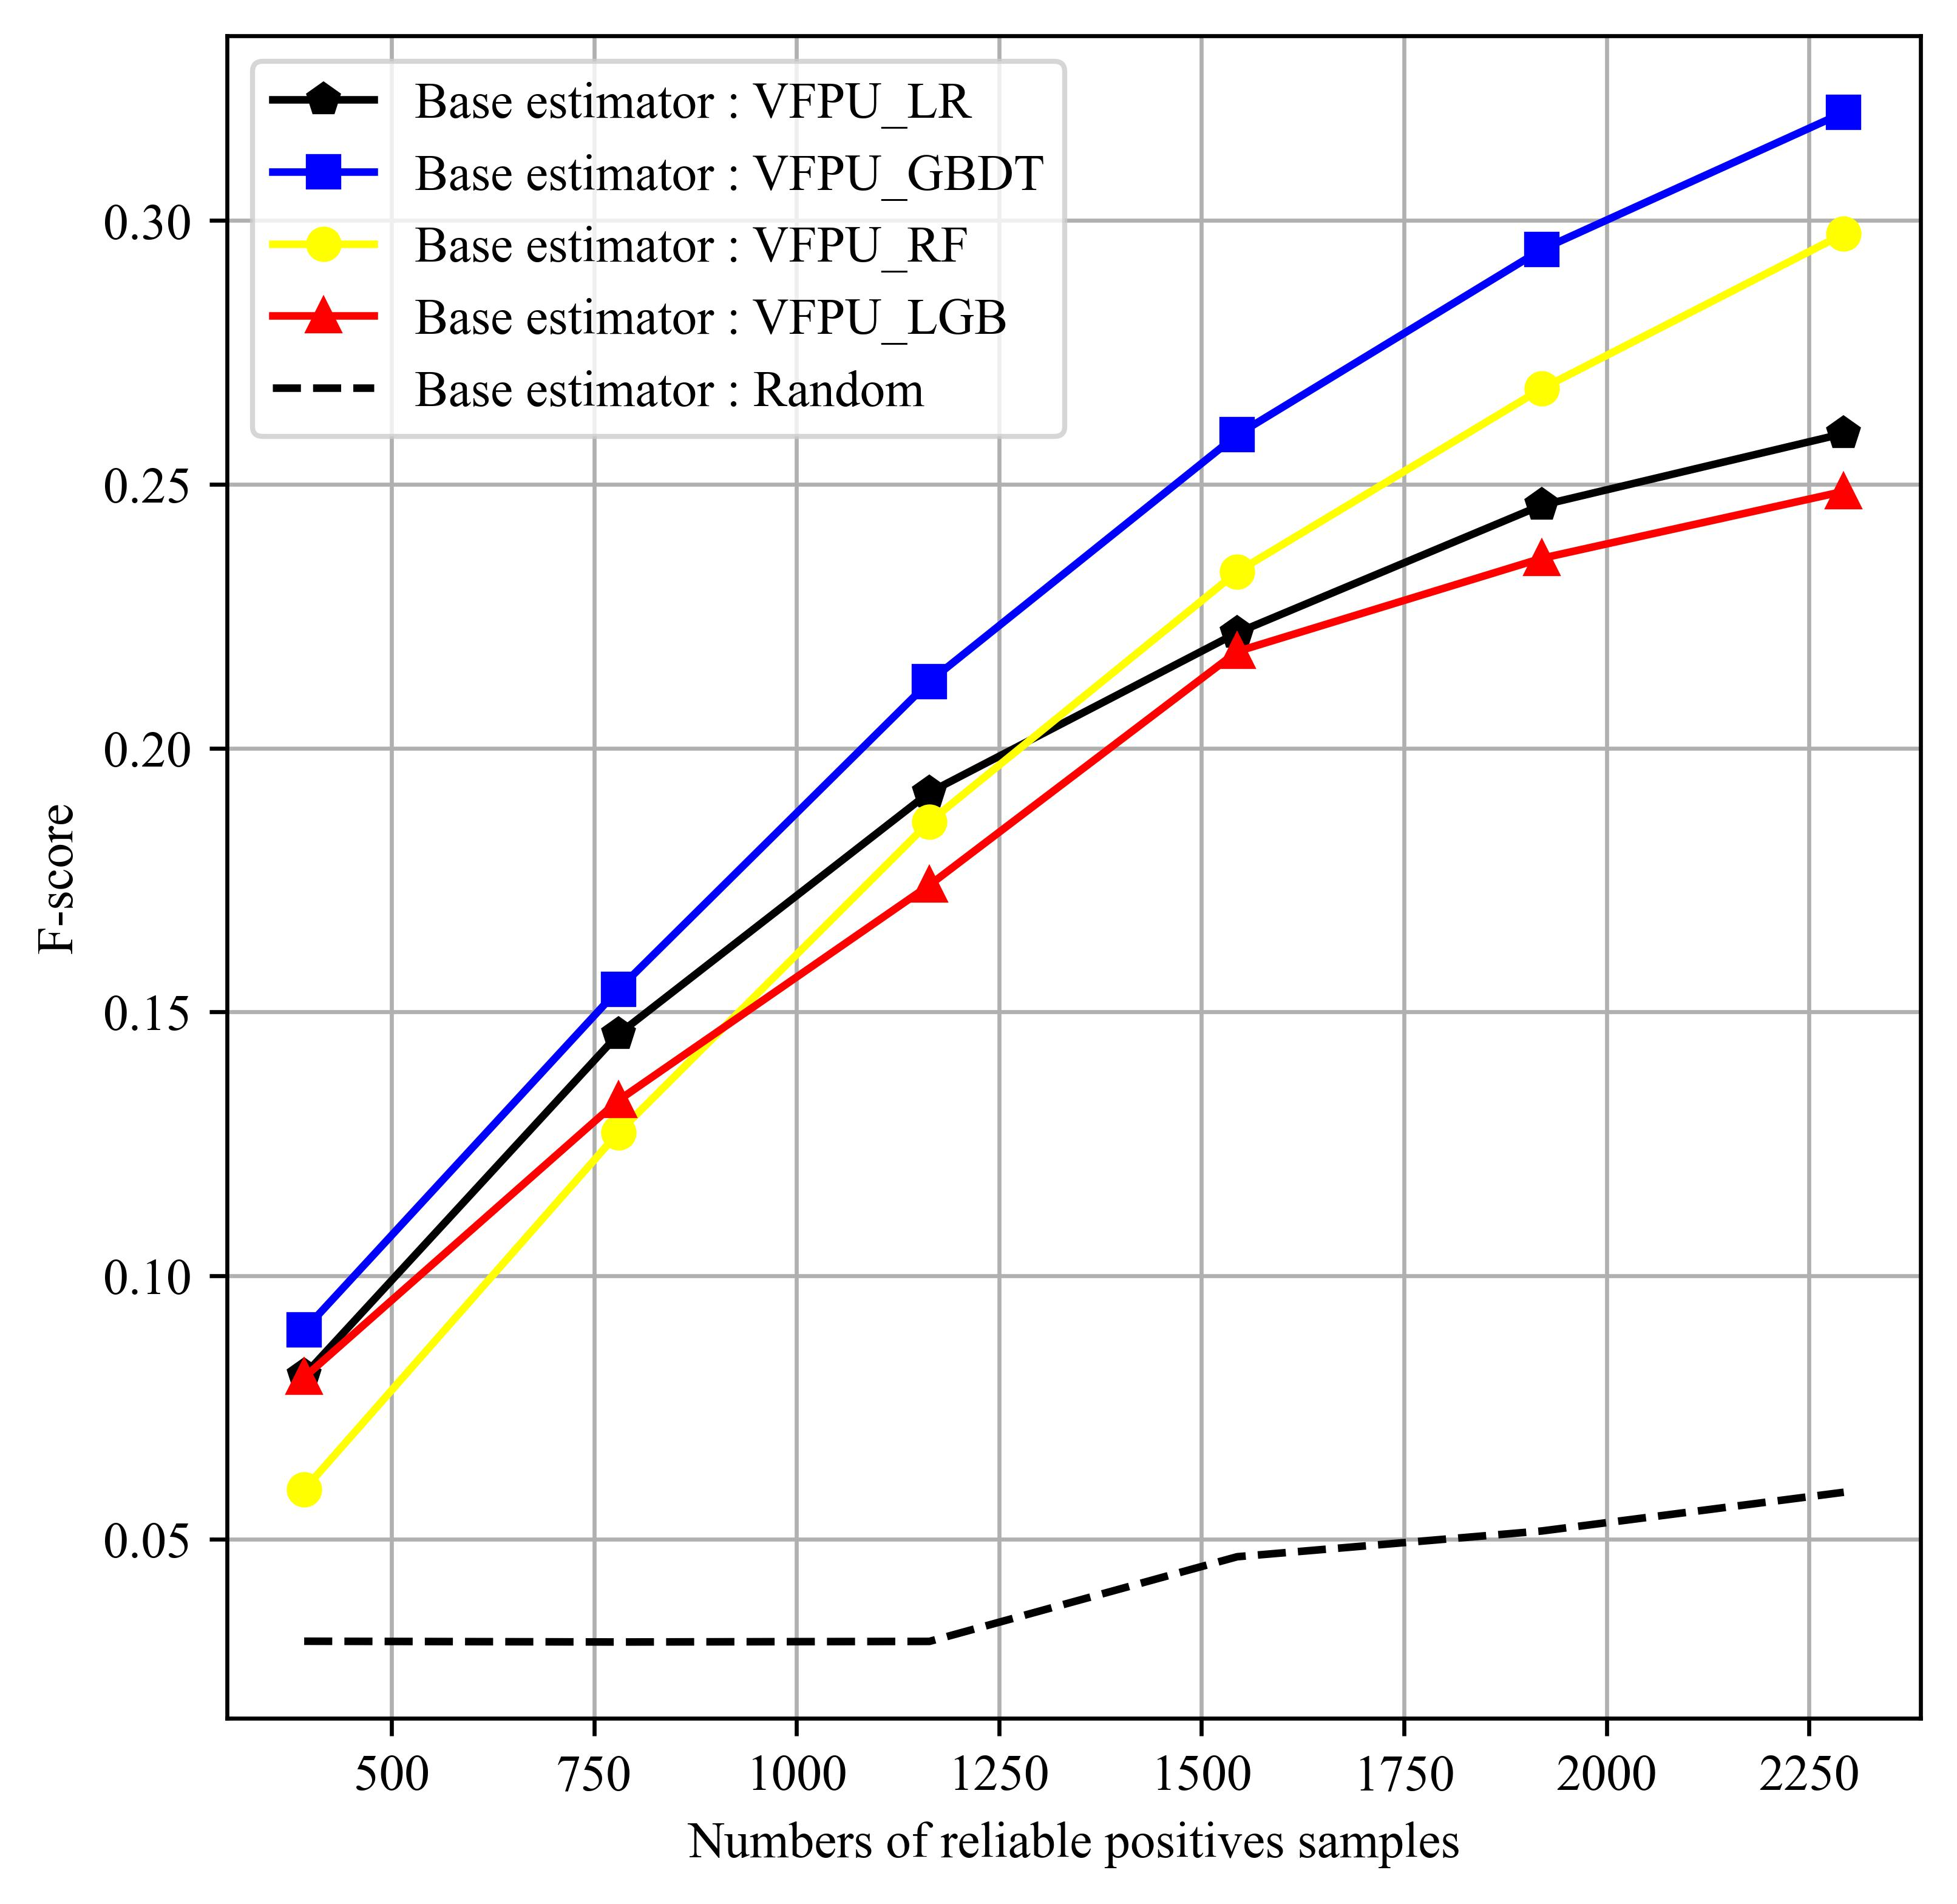
\includegraphics[width=0.45\textwidth,height=5.1cm]{chapters/imgs/Figure 2 (3) in JEPG format}}
	\subfigure[]{\label{RQ2.1.sub4}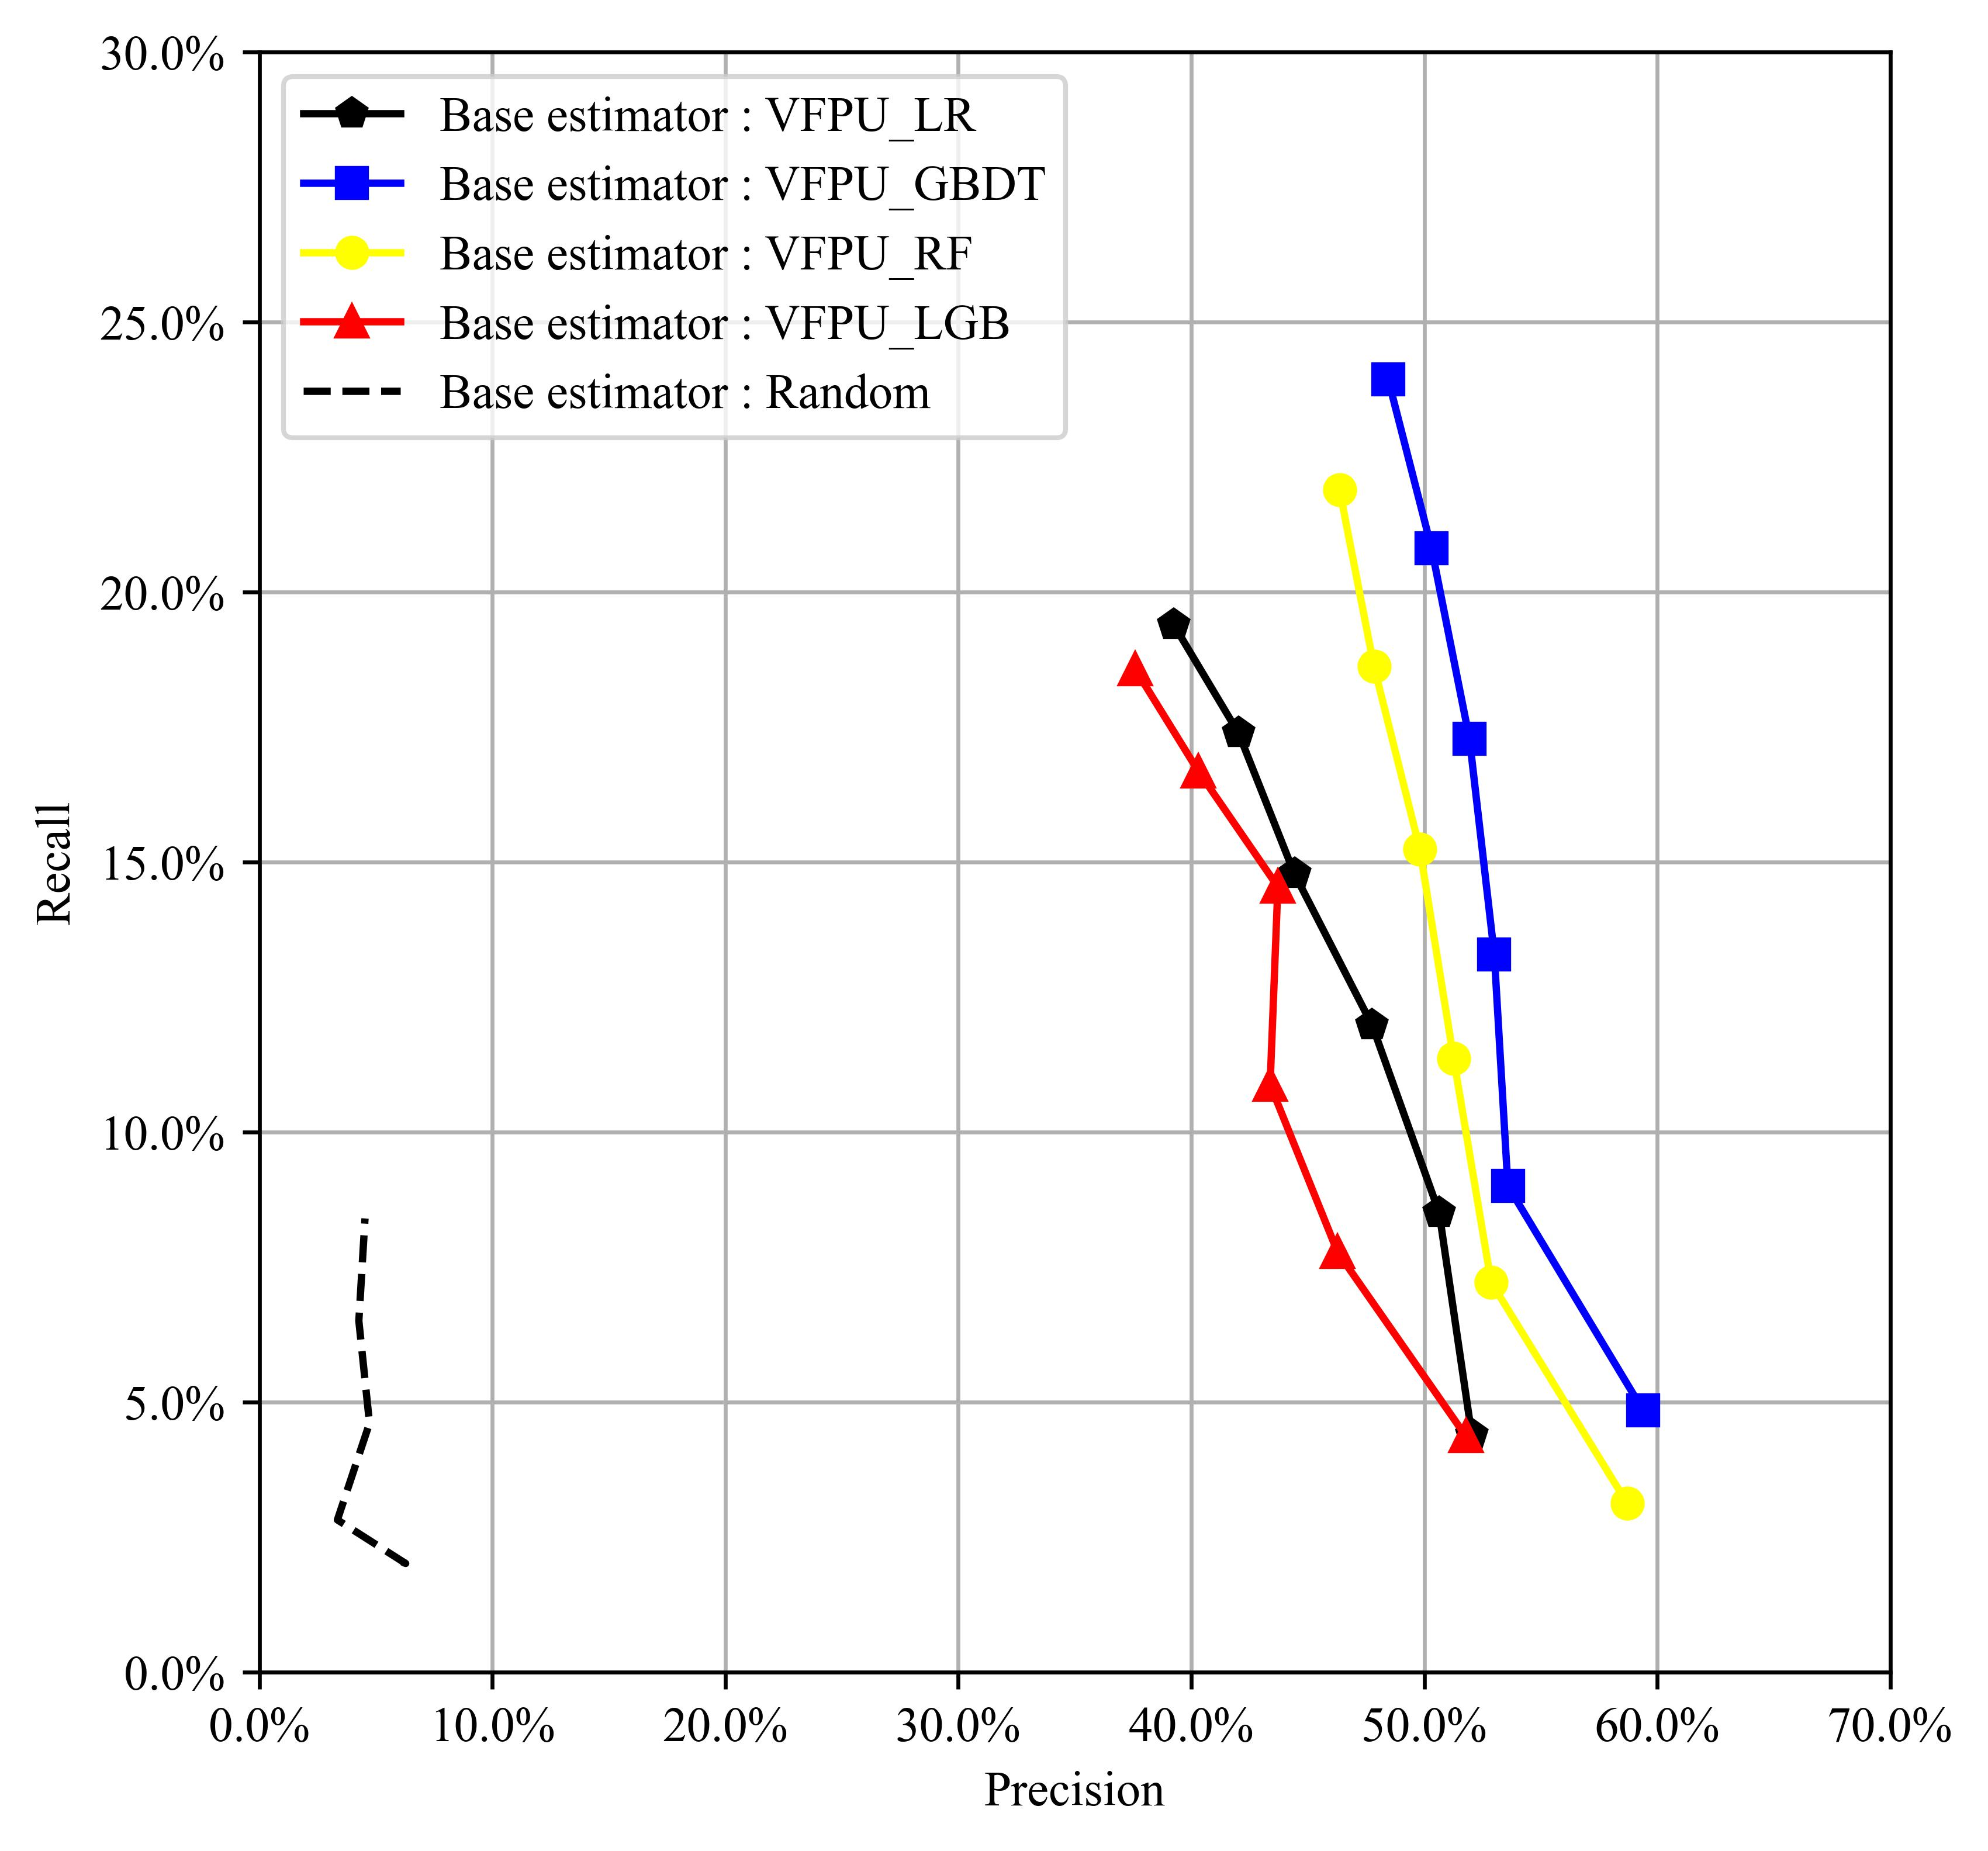
\includegraphics[width=0.45\textwidth,height=5.1cm]{chapters/imgs/Figure 2 (4) in JEPG format}}
	\begin{itemize}[leftmargin=1.6cm,rightmargin=1.6cm]
		\item[\quad] \bicaption[\xiaosi 不同基学器在不同可靠正样本数量下的性能]
		{\centering \songti \wuhao 不同基学器在不同可靠正样本数量下的性能:(a)精度;(b)召回率;(c)F-score;(d)精度-召回率(Bank 数据集)}
		{\centering \wuhao Performance of Different Base Estimators with Varying Reliable Positive Samples: (a) Precision; (b) Recall; (c) F-score; (d) Precision-Recall (The Bank Marketing Dataset)}
	\end{itemize}
	\label{RQ2.1}
\end{figure}

\begin{figure}[!htbp]
    \centering
    \vspace{0.5cm} % 调整图片与上文的间距
    \captionsetup{size=footnotesize}

    \subfigure[]{\label{RQ2.2.sub1}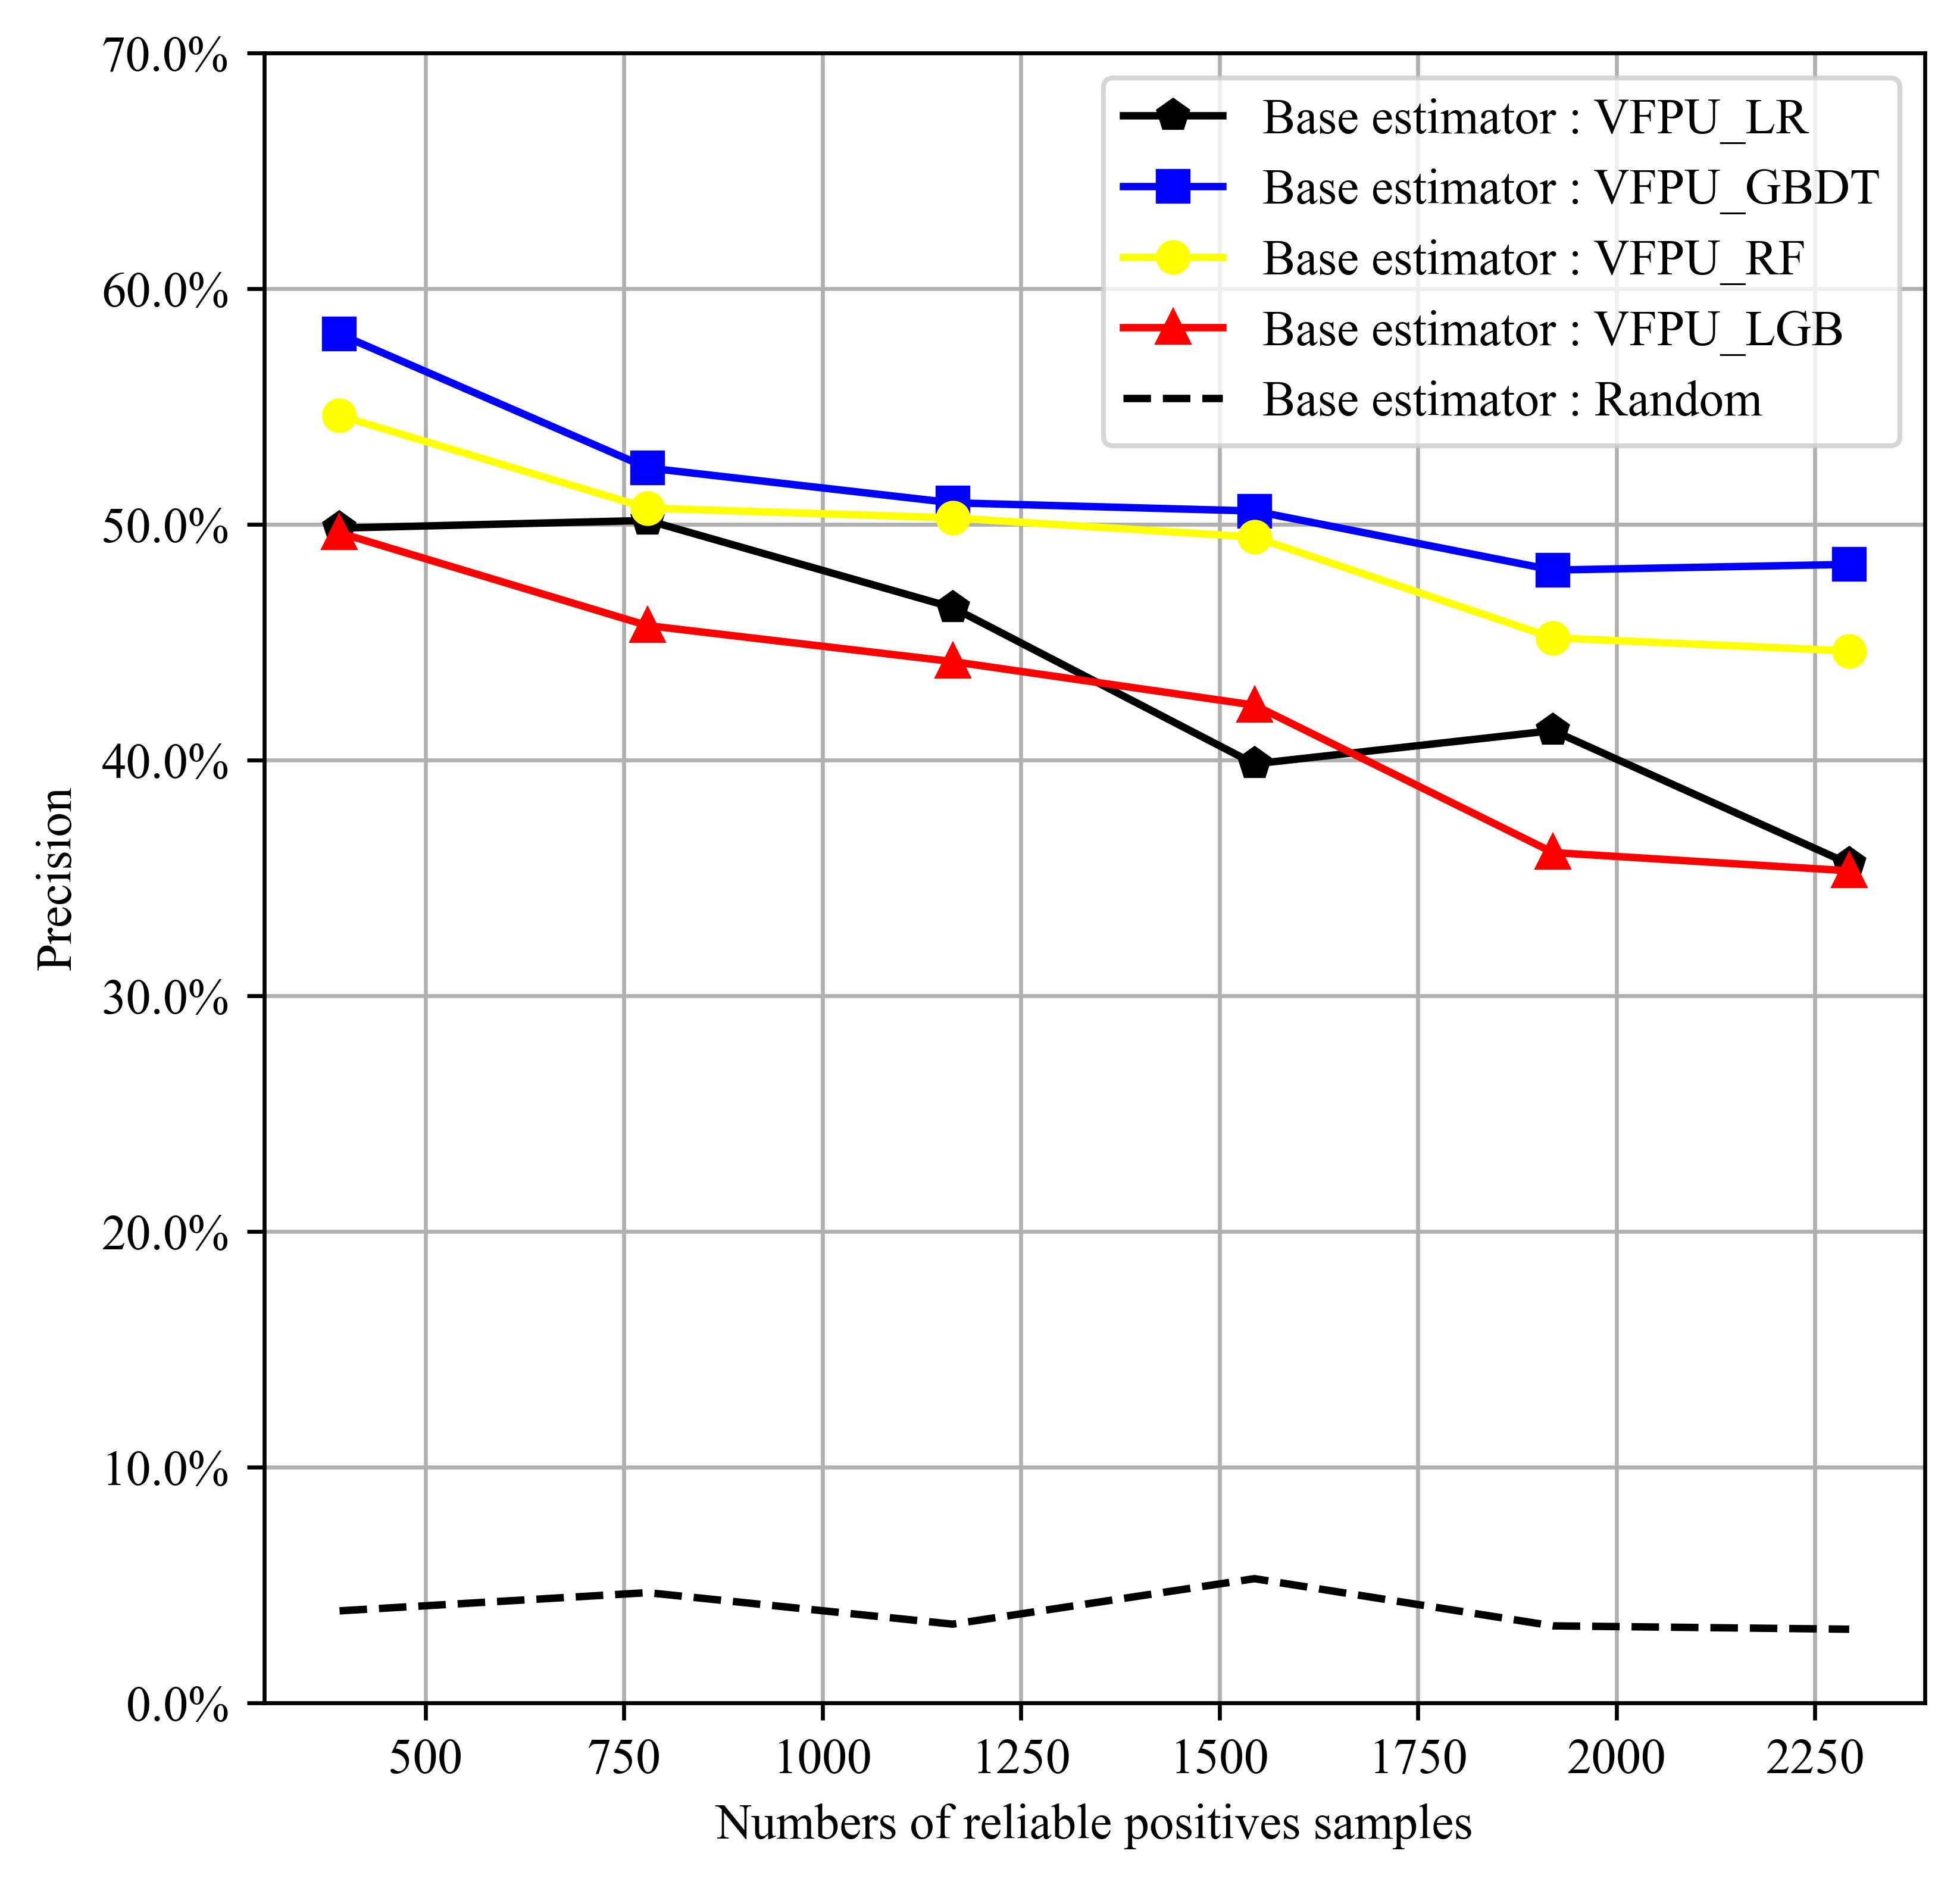
\includegraphics[width=0.45\textwidth,height=5.1cm]{chapters/imgs/Figure 3 (1) in JEPG format}}
    \subfigure[]{\label{RQ2.2.sub2}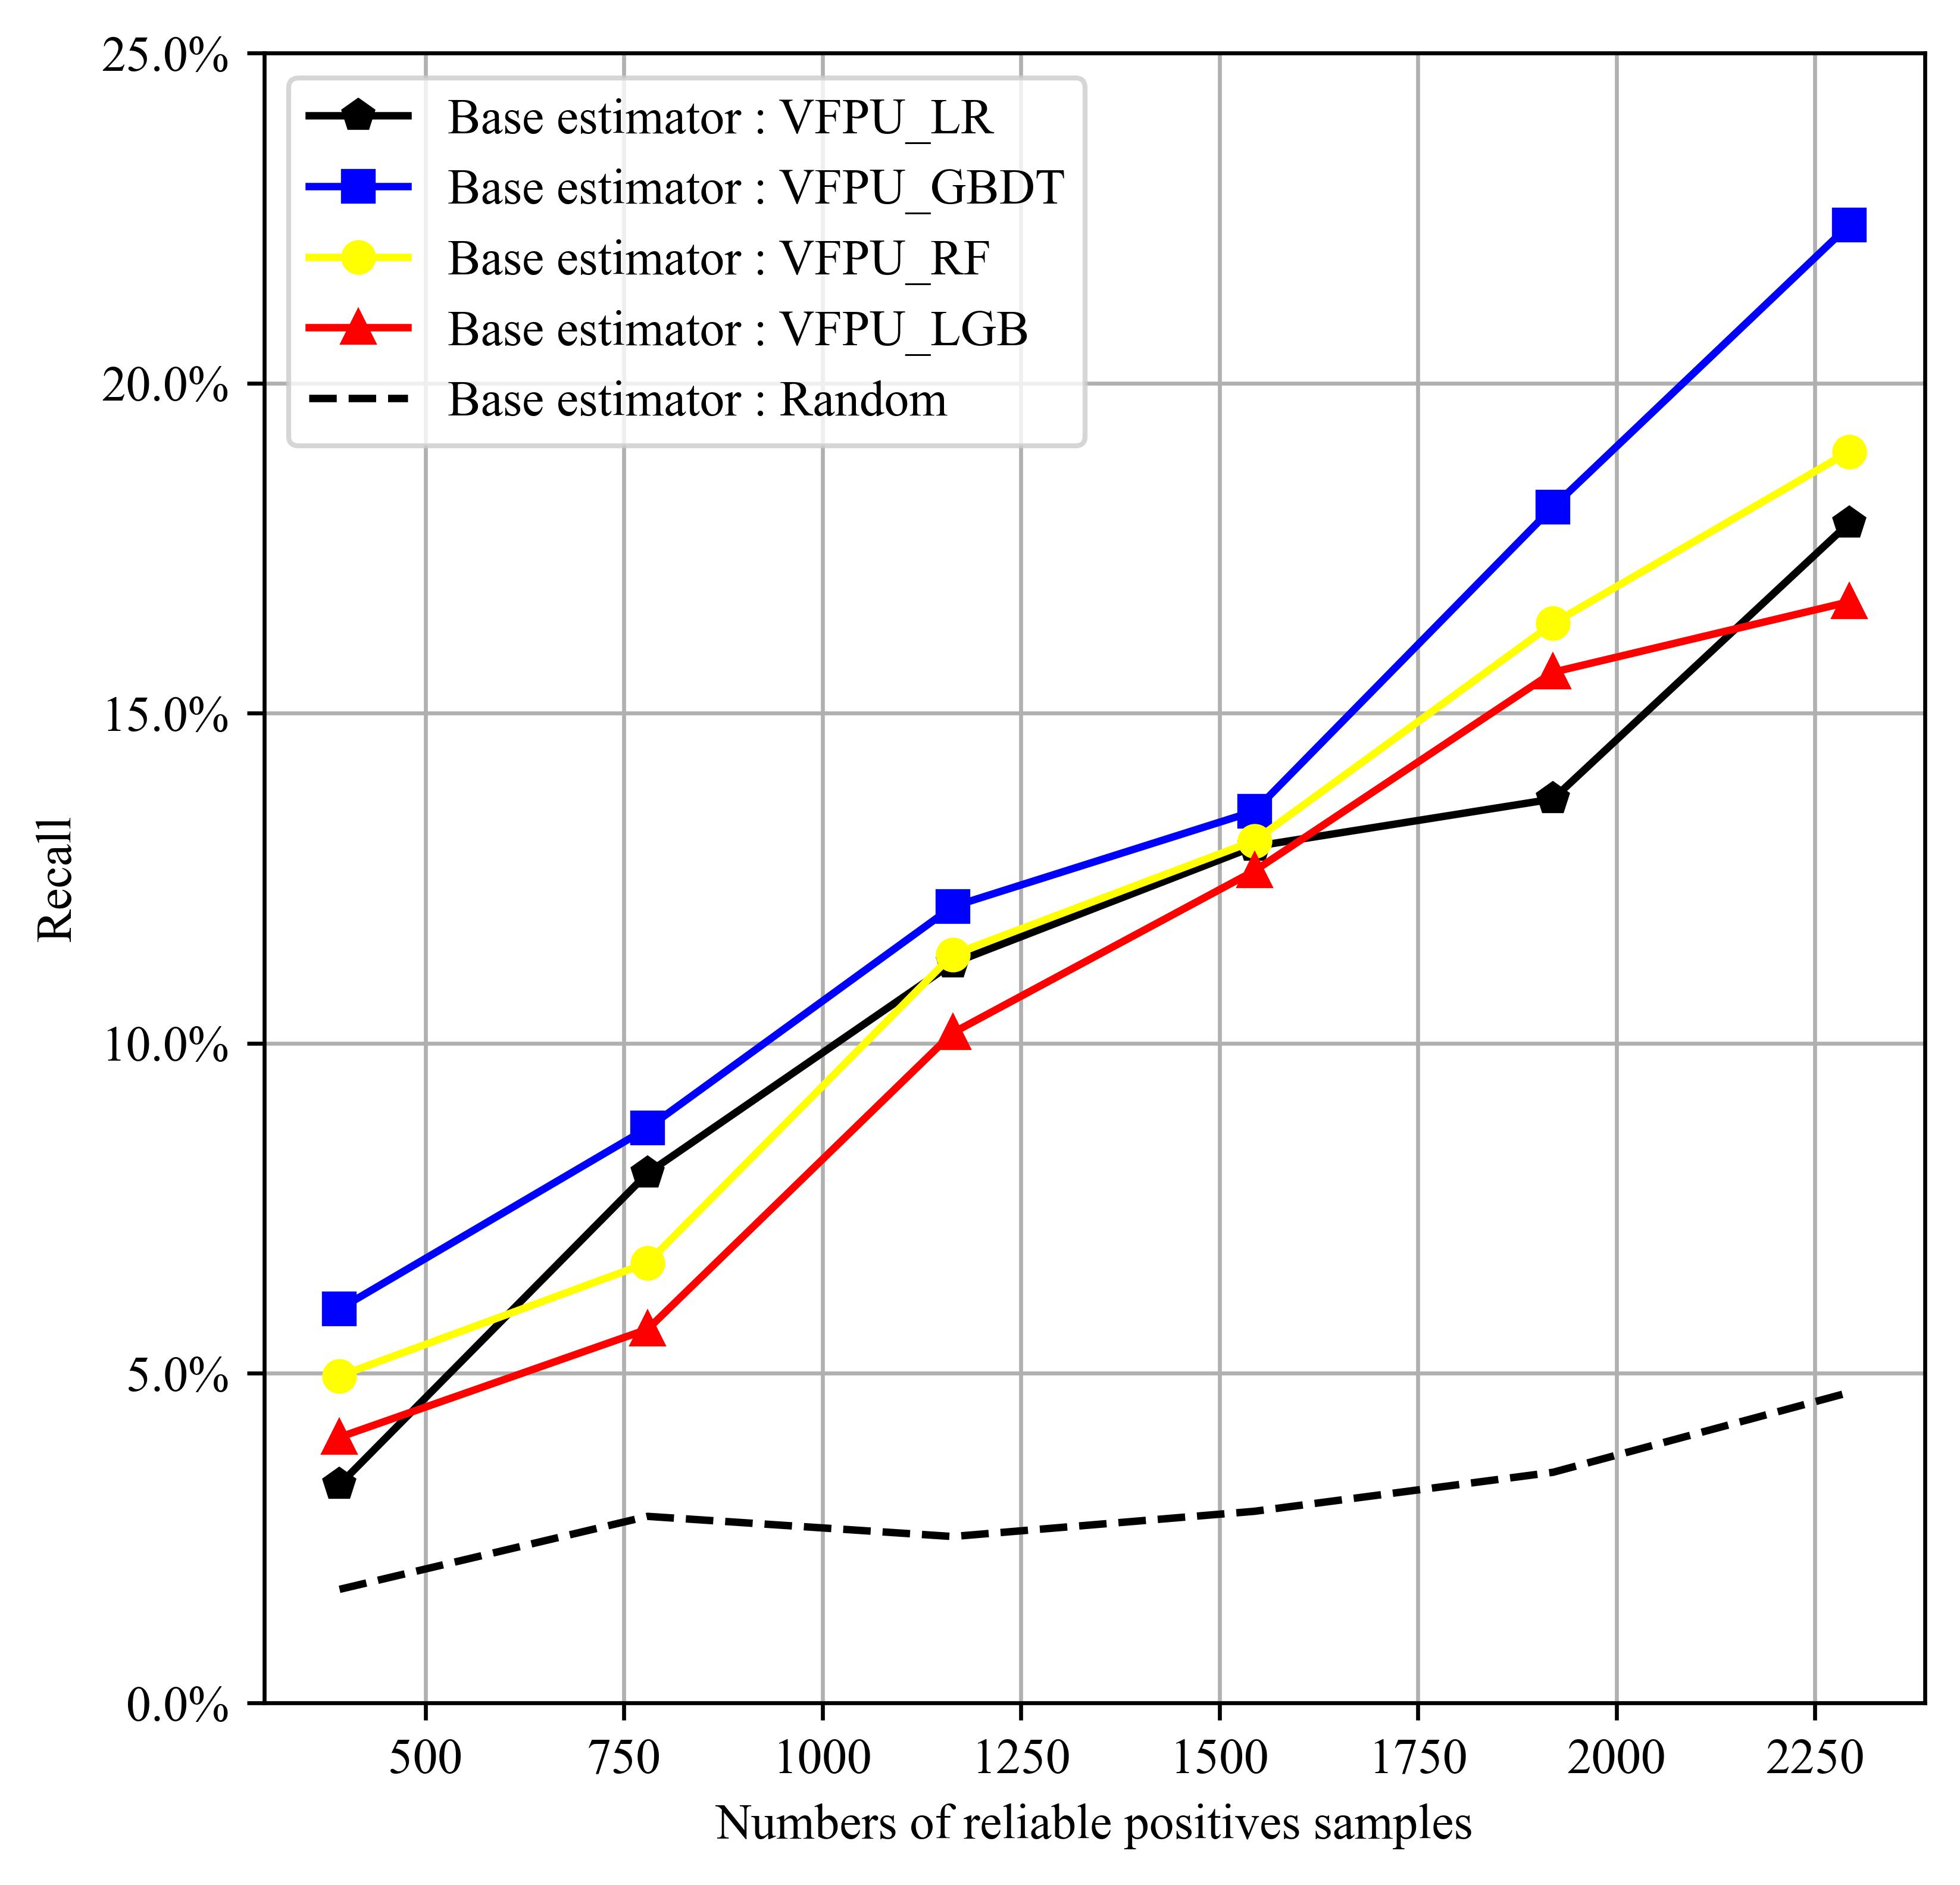
\includegraphics[width=0.45\textwidth,height=5.1cm]{chapters/imgs/Figure 3 (2) in JEPG format}}
    \subfigure[]{\label{RQ2.2.sub3}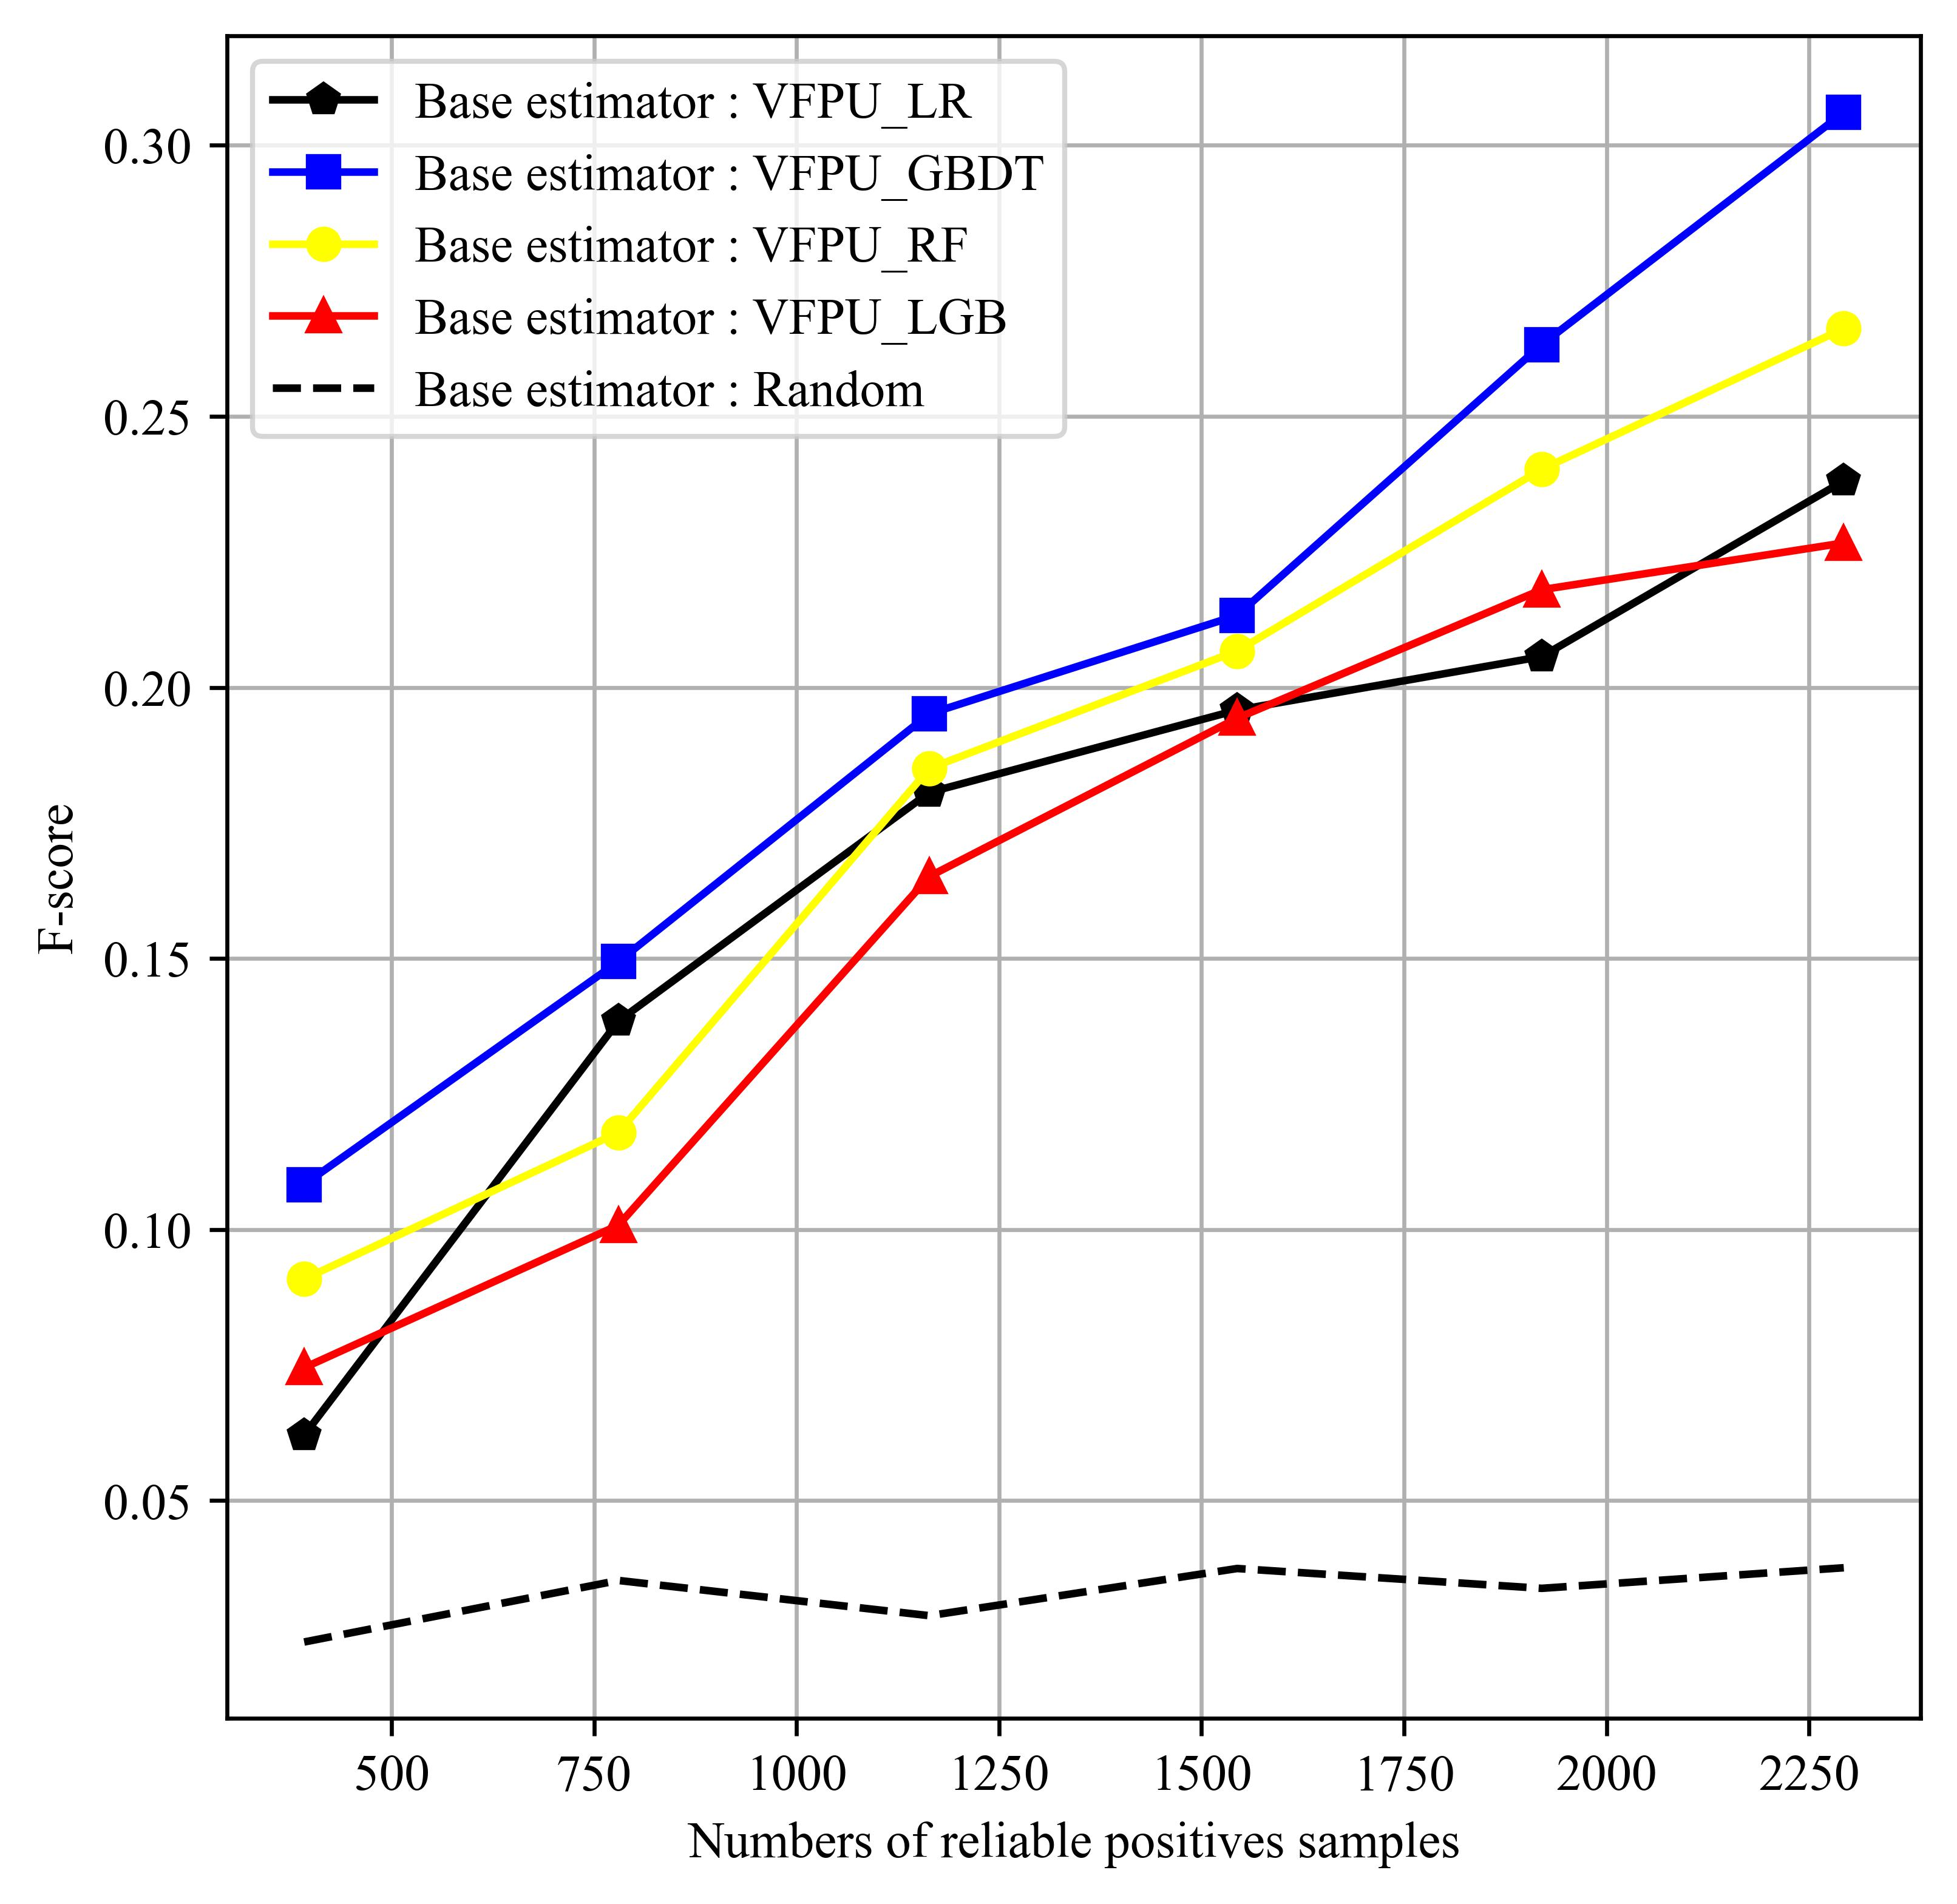
\includegraphics[width=0.45\textwidth,height=5.1cm]{chapters/imgs/Figure 3 (3) in JEPG format}}
    \subfigure[]{\label{RQ2.2.sub4}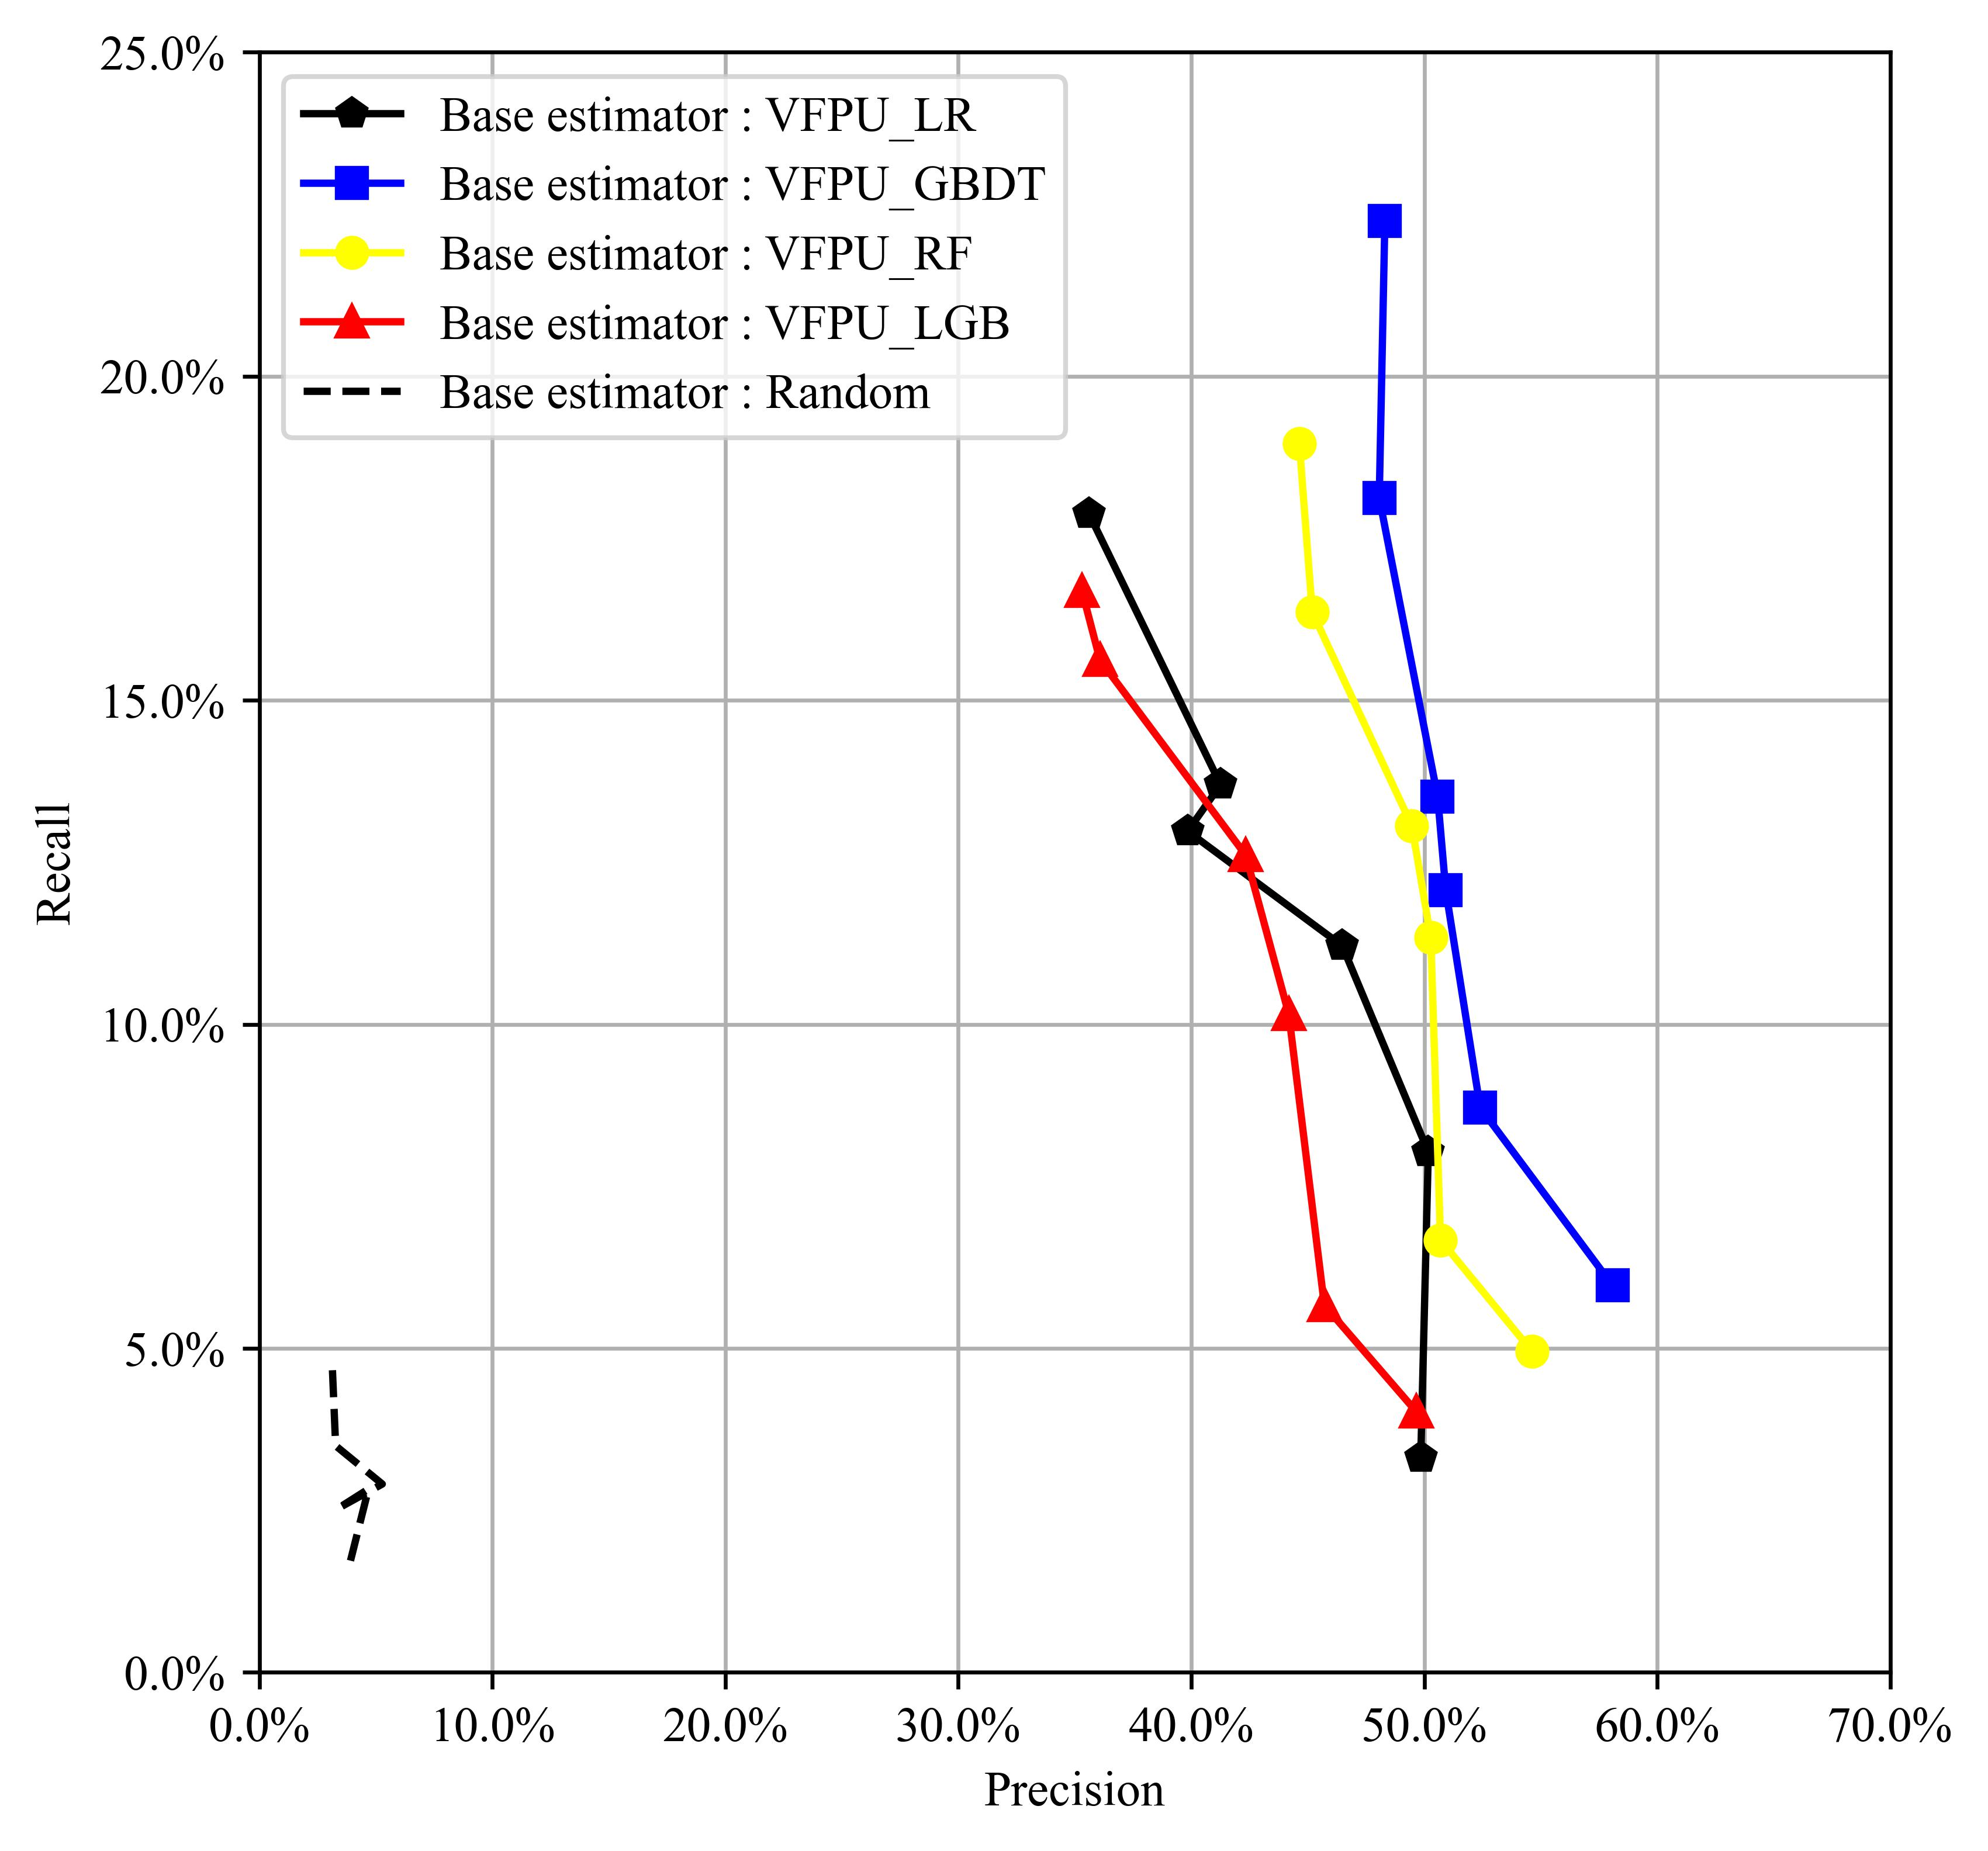
\includegraphics[width=0.45\textwidth,height=5.1cm]{chapters/imgs/Figure 3 (4) in JEPG format}}
    \begin{itemize}[leftmargin=1.6cm,rightmargin=1.6cm]
        \item[\quad] \bicaption[\xiaosi 不同基学器在不同可靠正样本数量下的性能]
        {\centering \songti \wuhao 不同基学器在不同可靠正样本数量下的性能:(a)精度;(b)召回率;(c)F-score;(d)精度-召回率(Credit 数据集)}
        {\centering \wuhao Performance of Different Base Estimators with Varying Reliable Positive Samples: (a) Precision; (b) Recall; (c) F-score; (d) Precision-Recall (The Default of Credit Card Clients Dataset)}
    \end{itemize}
    \label{RQ2.2}
\end{figure}

\begin{figure}[!htbp]
    \centering
    \vspace{0.5cm} % 调整图片与上文的间距
    \captionsetup{size=footnotesize}

    \subfigure[]{\label{RQ2.3.sub1}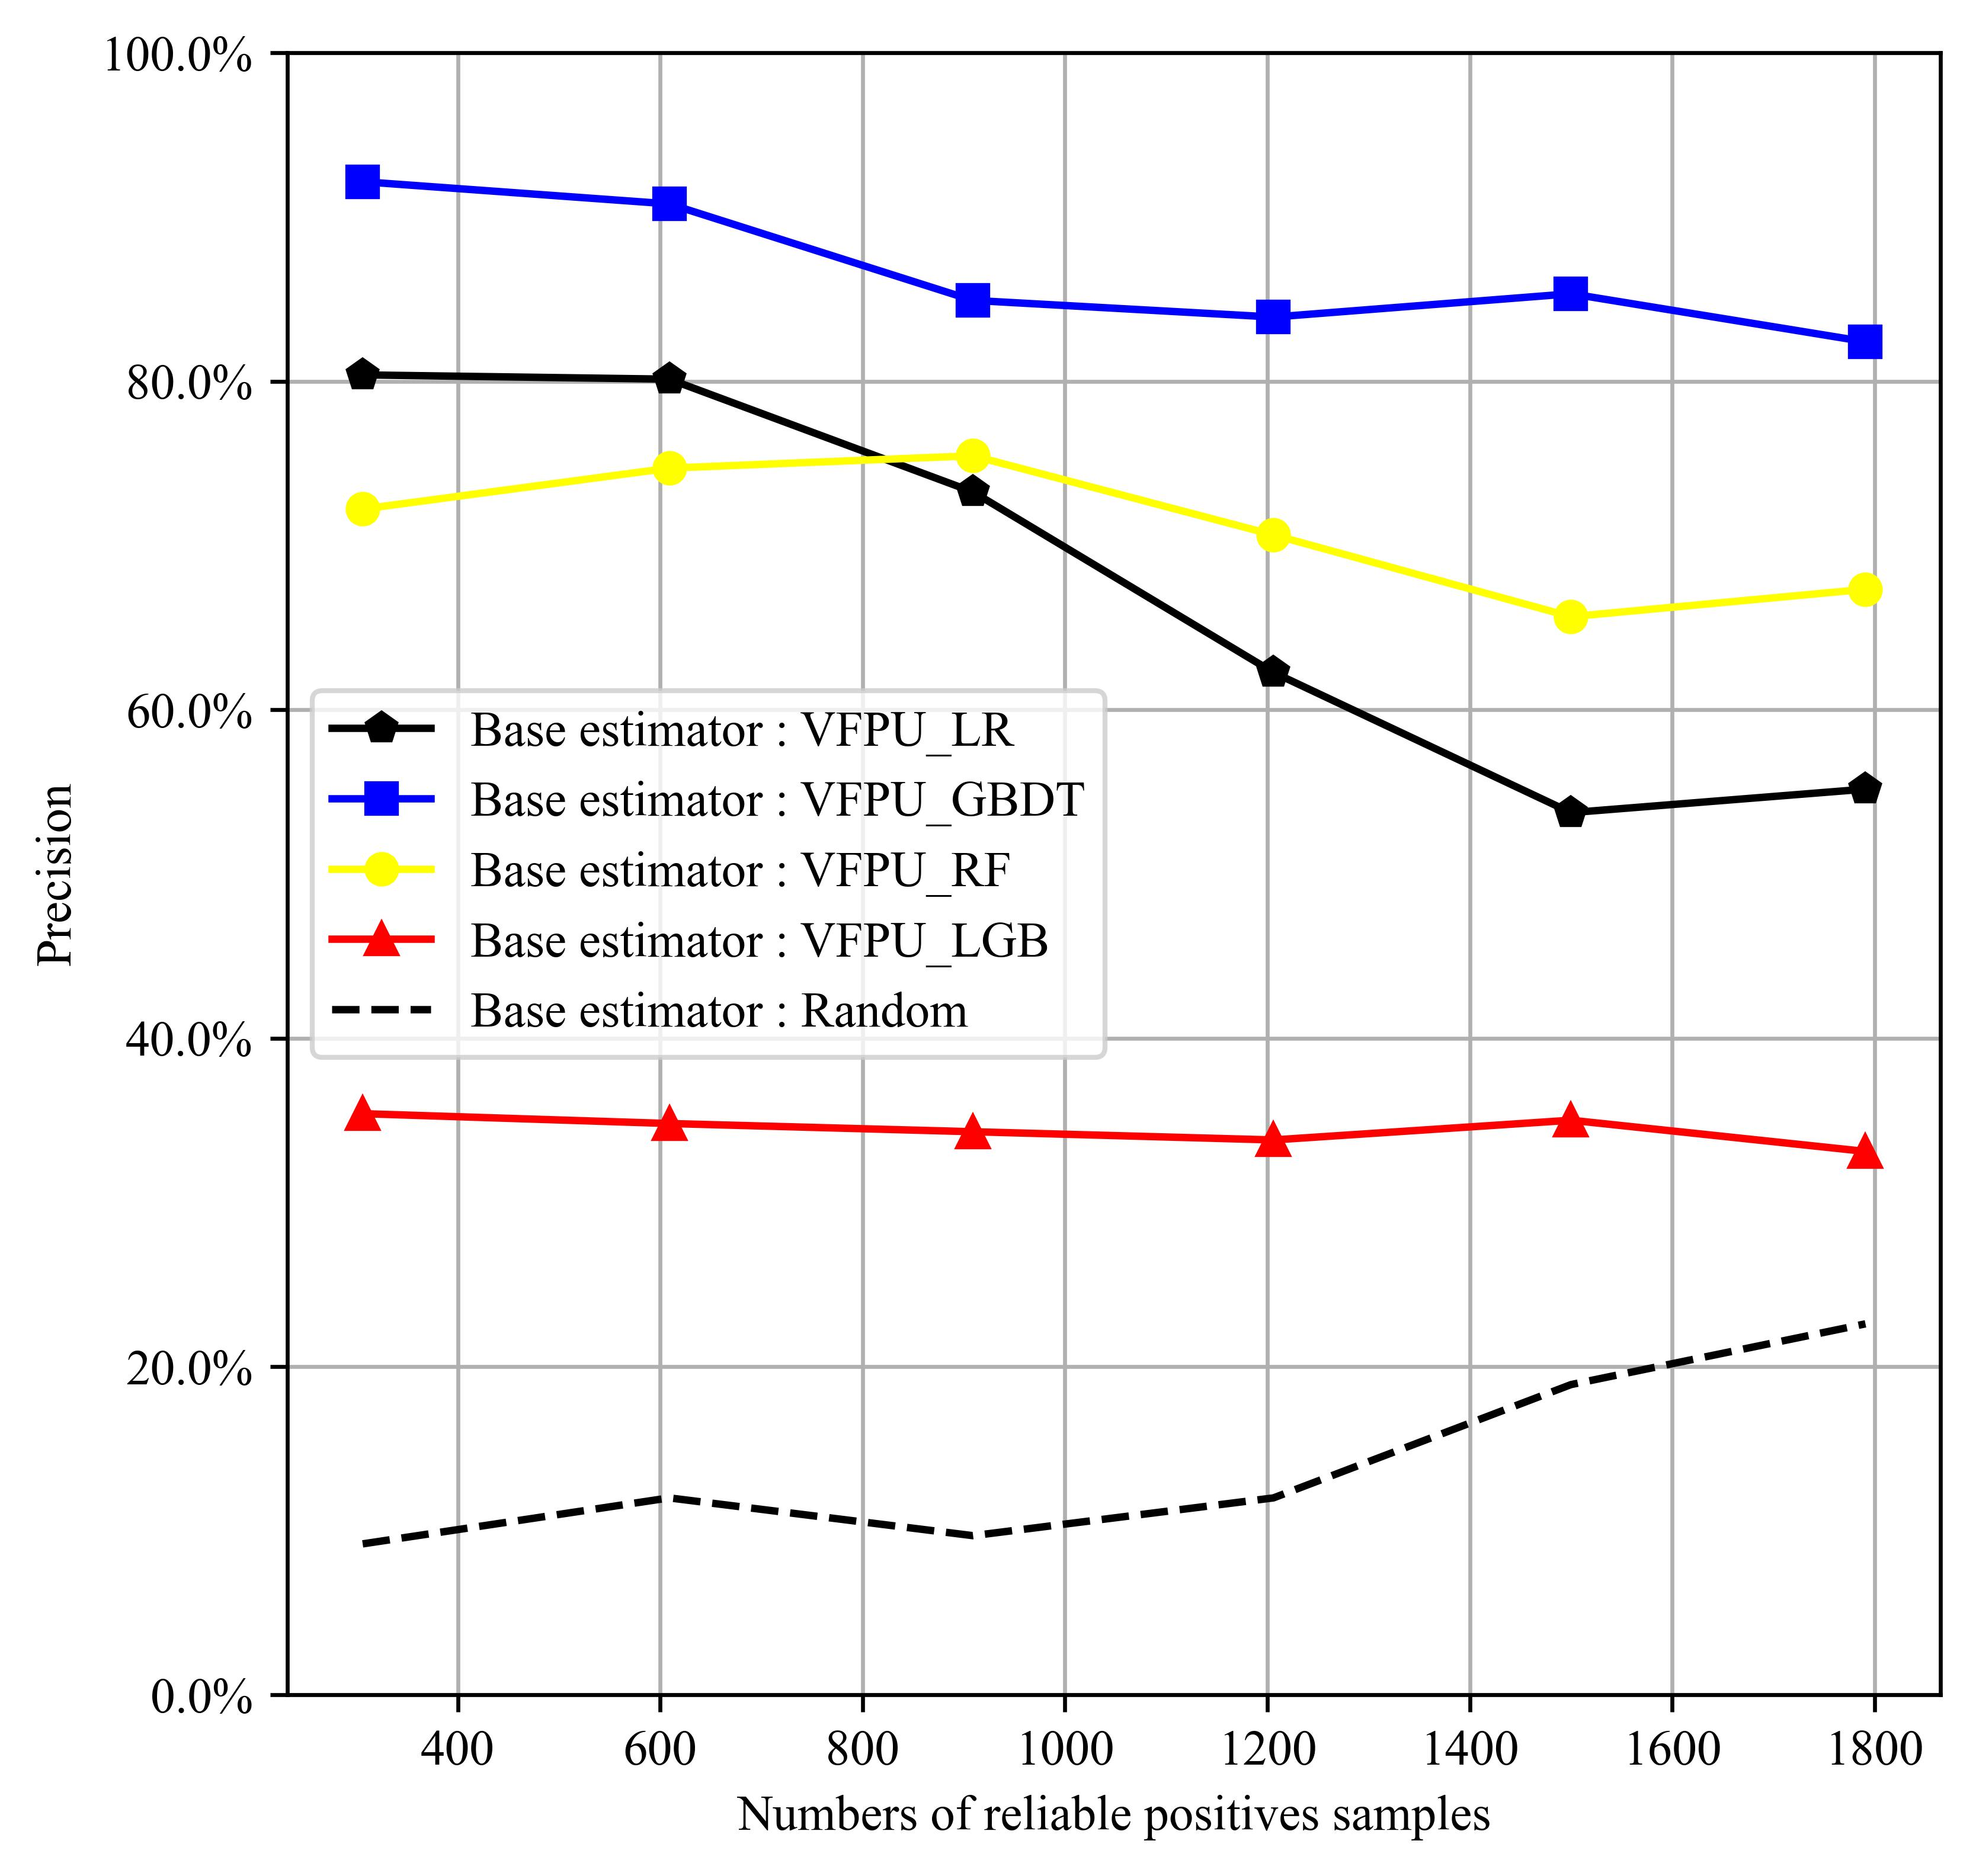
\includegraphics[width=0.45\textwidth,height=5.1cm]{chapters/imgs/Figure 4 (1) in JEPG format}}
    \subfigure[]{\label{RQ2.3.sub2}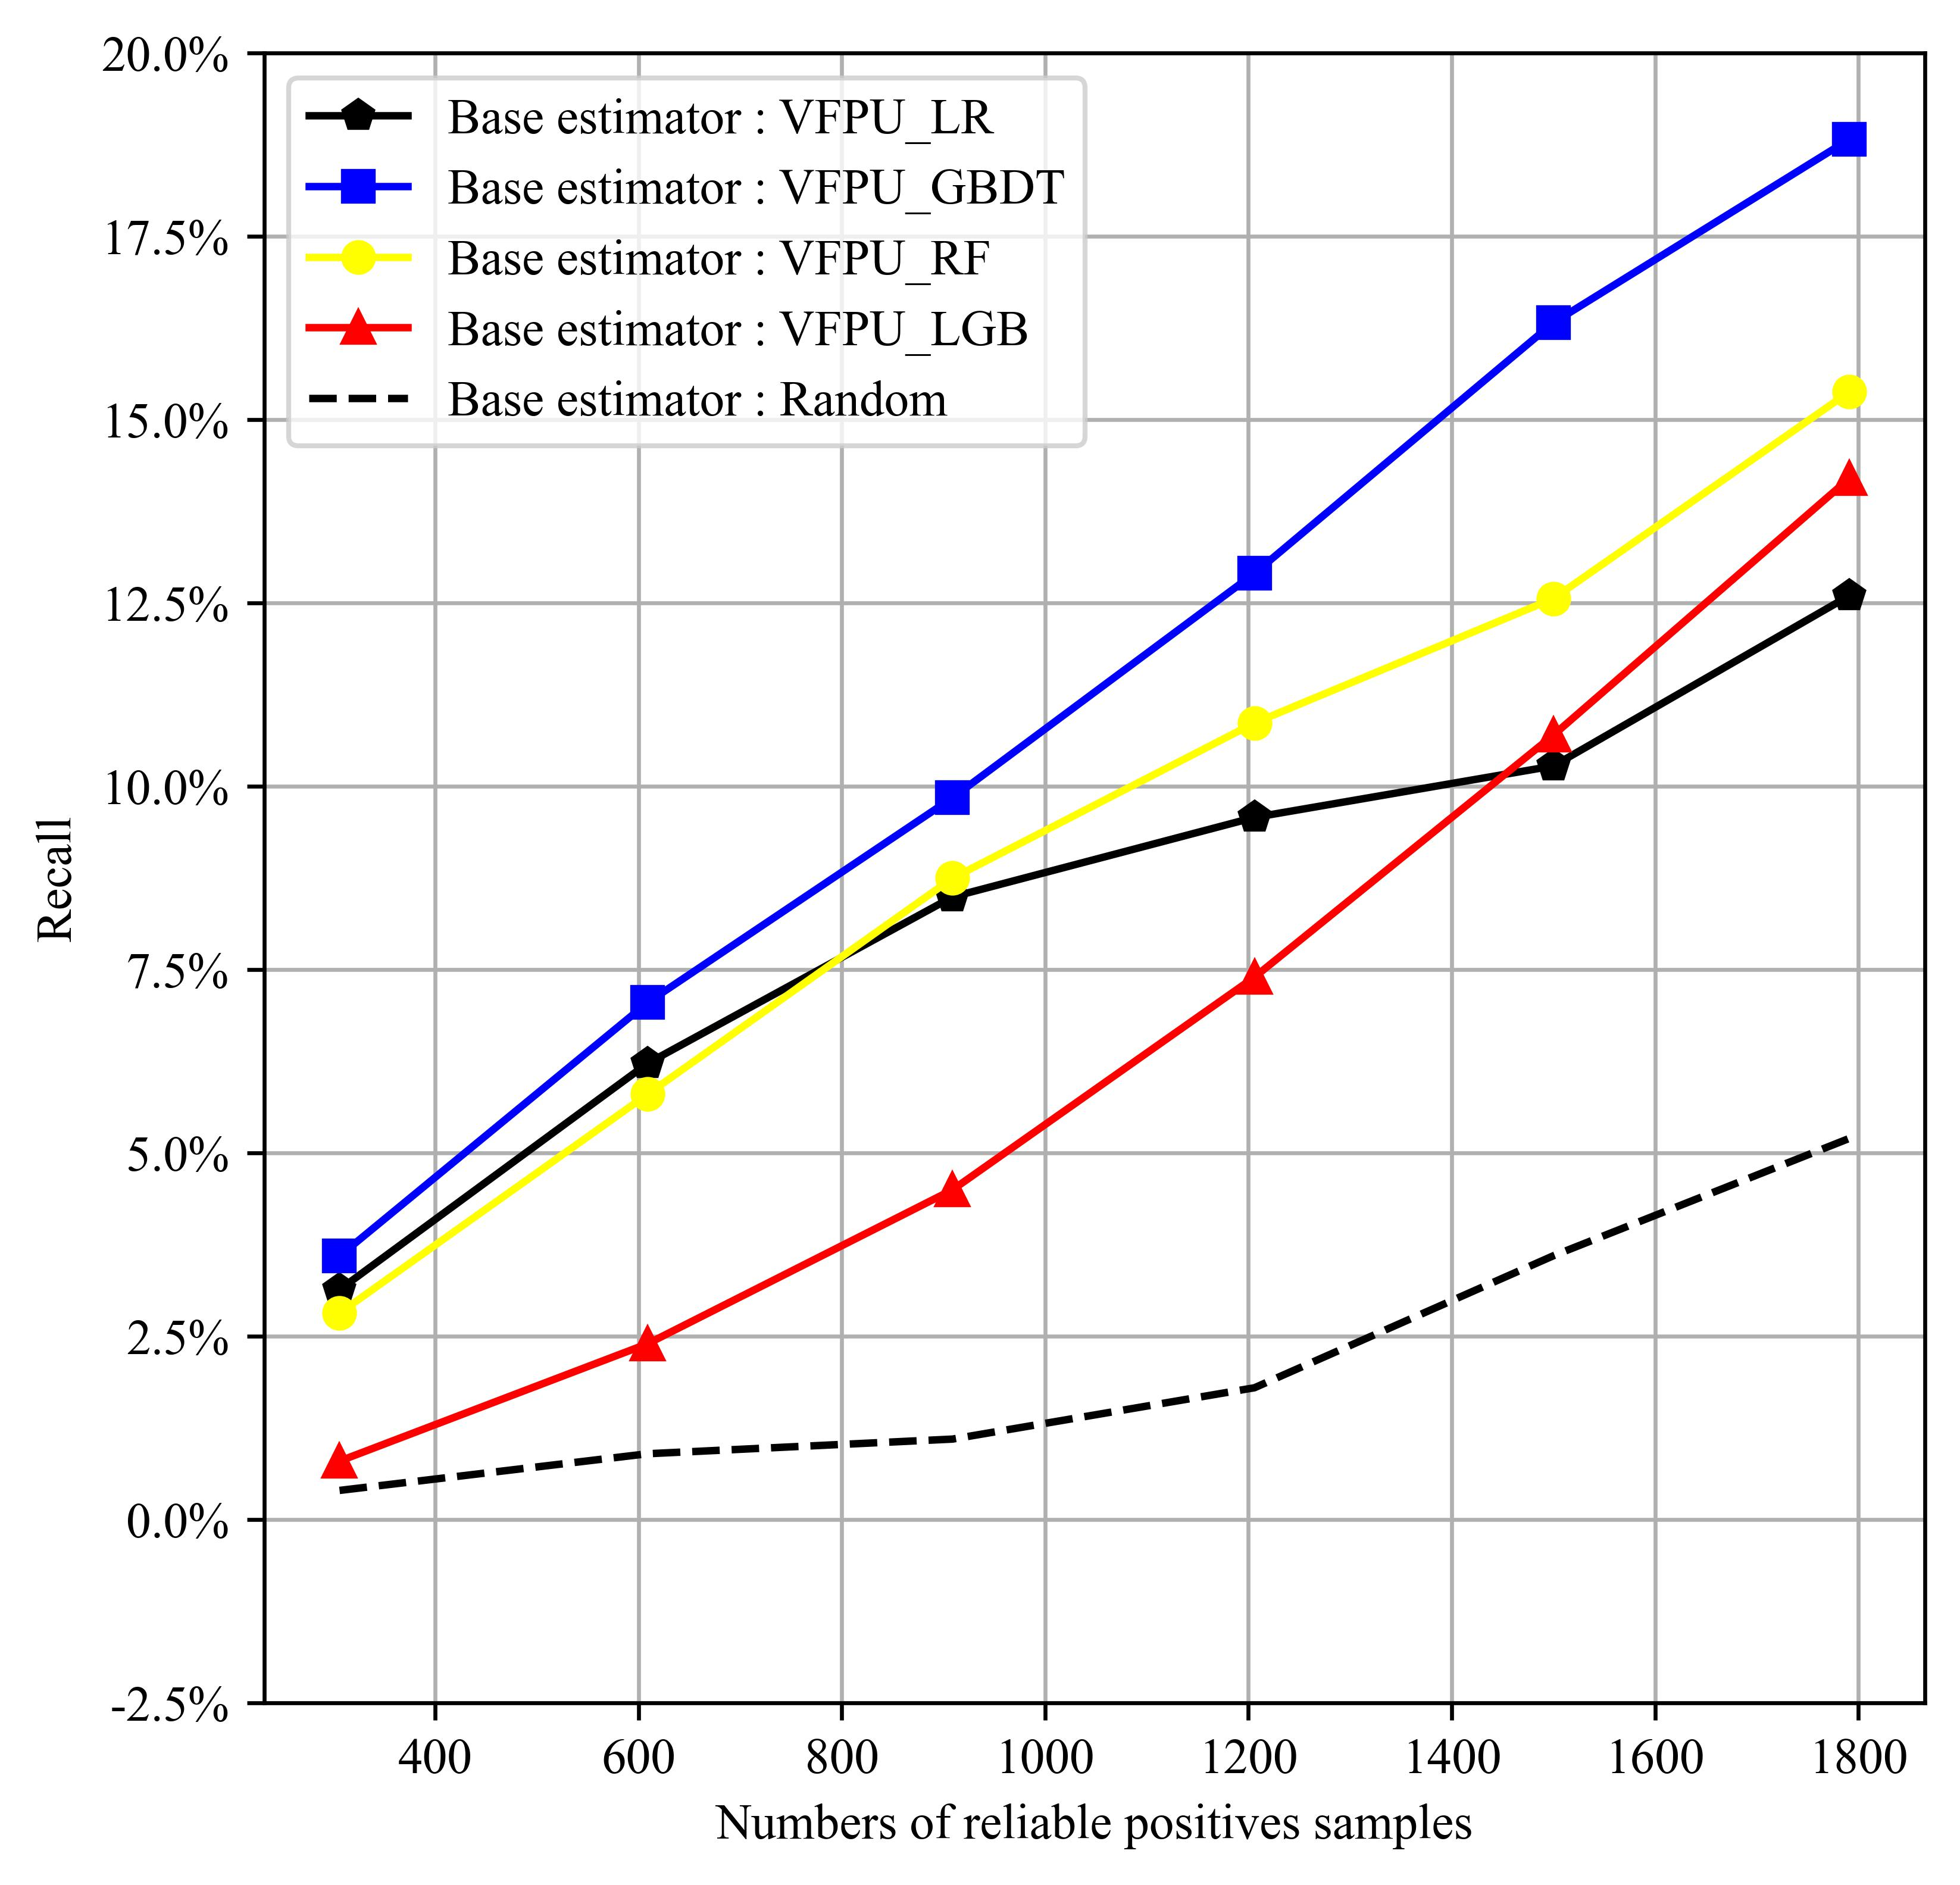
\includegraphics[width=0.45\textwidth,height=5.1cm]{chapters/imgs/Figure 4 (2) in JEPG format}}
    \subfigure[]{\label{RQ2.3.sub3}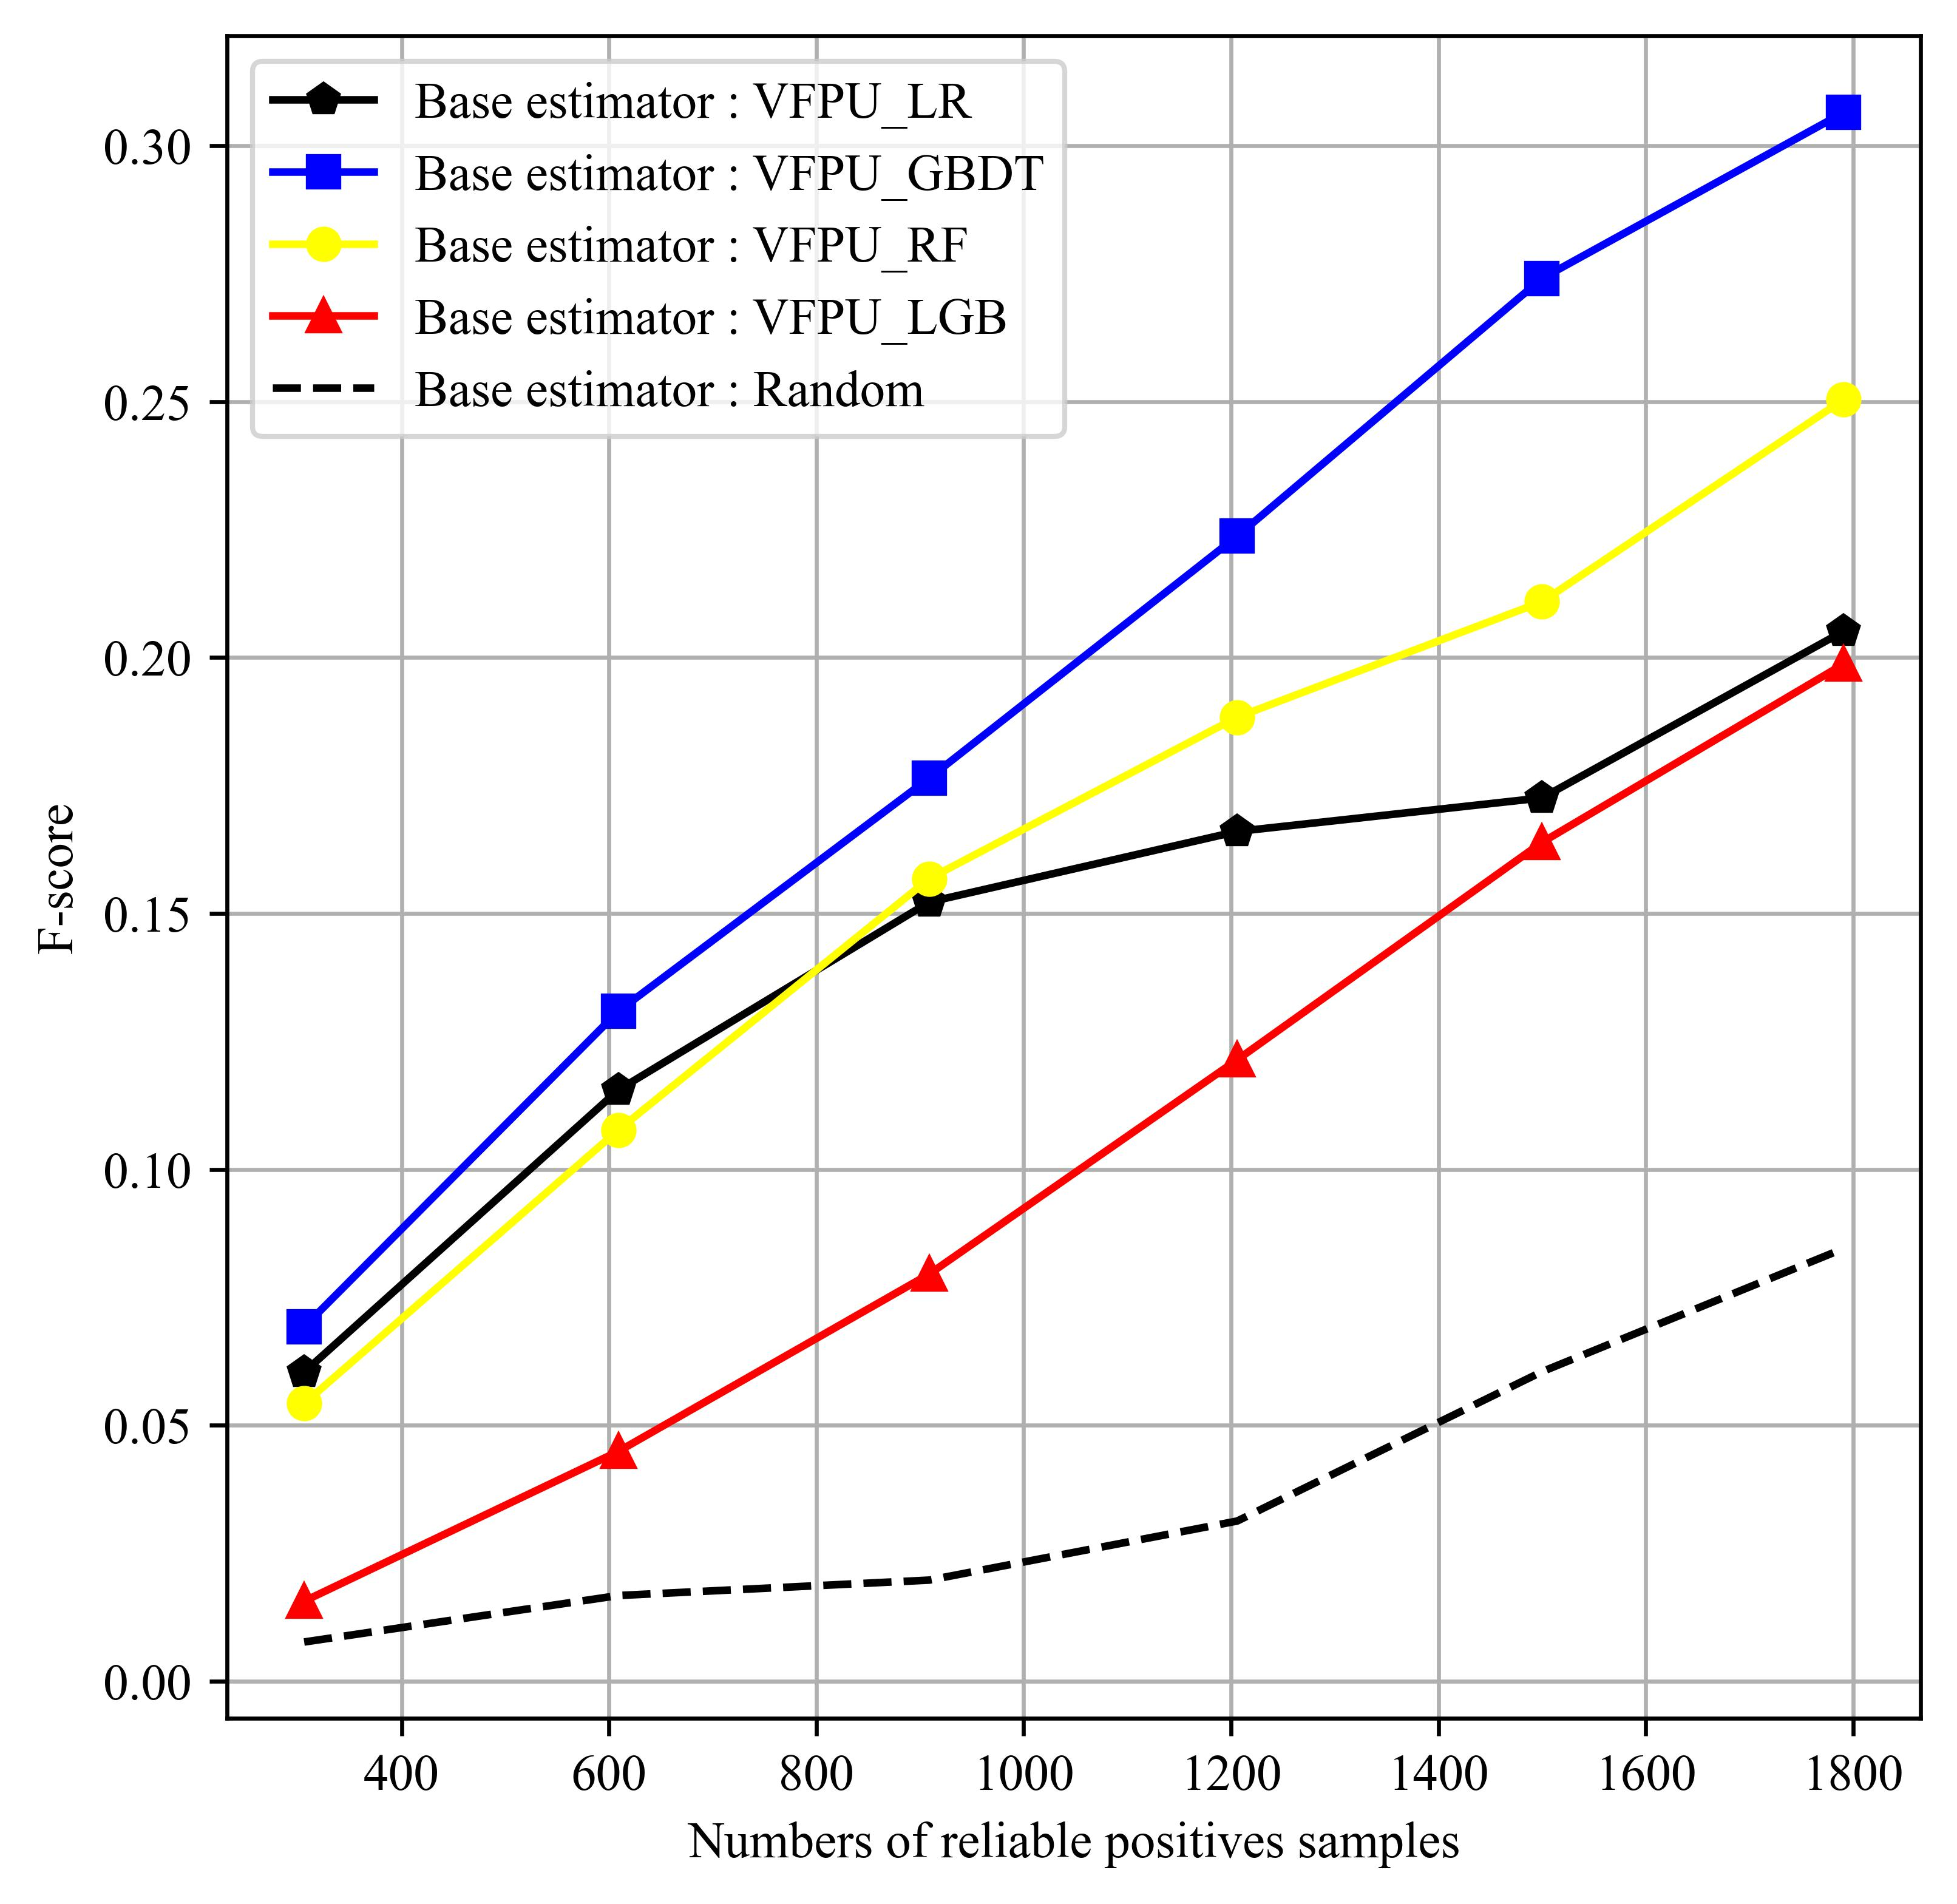
\includegraphics[width=0.45\textwidth,height=5.1cm]{chapters/imgs/Figure 4 (3) in JEPG format}}
    \subfigure[]{\label{RQ2.3.sub4}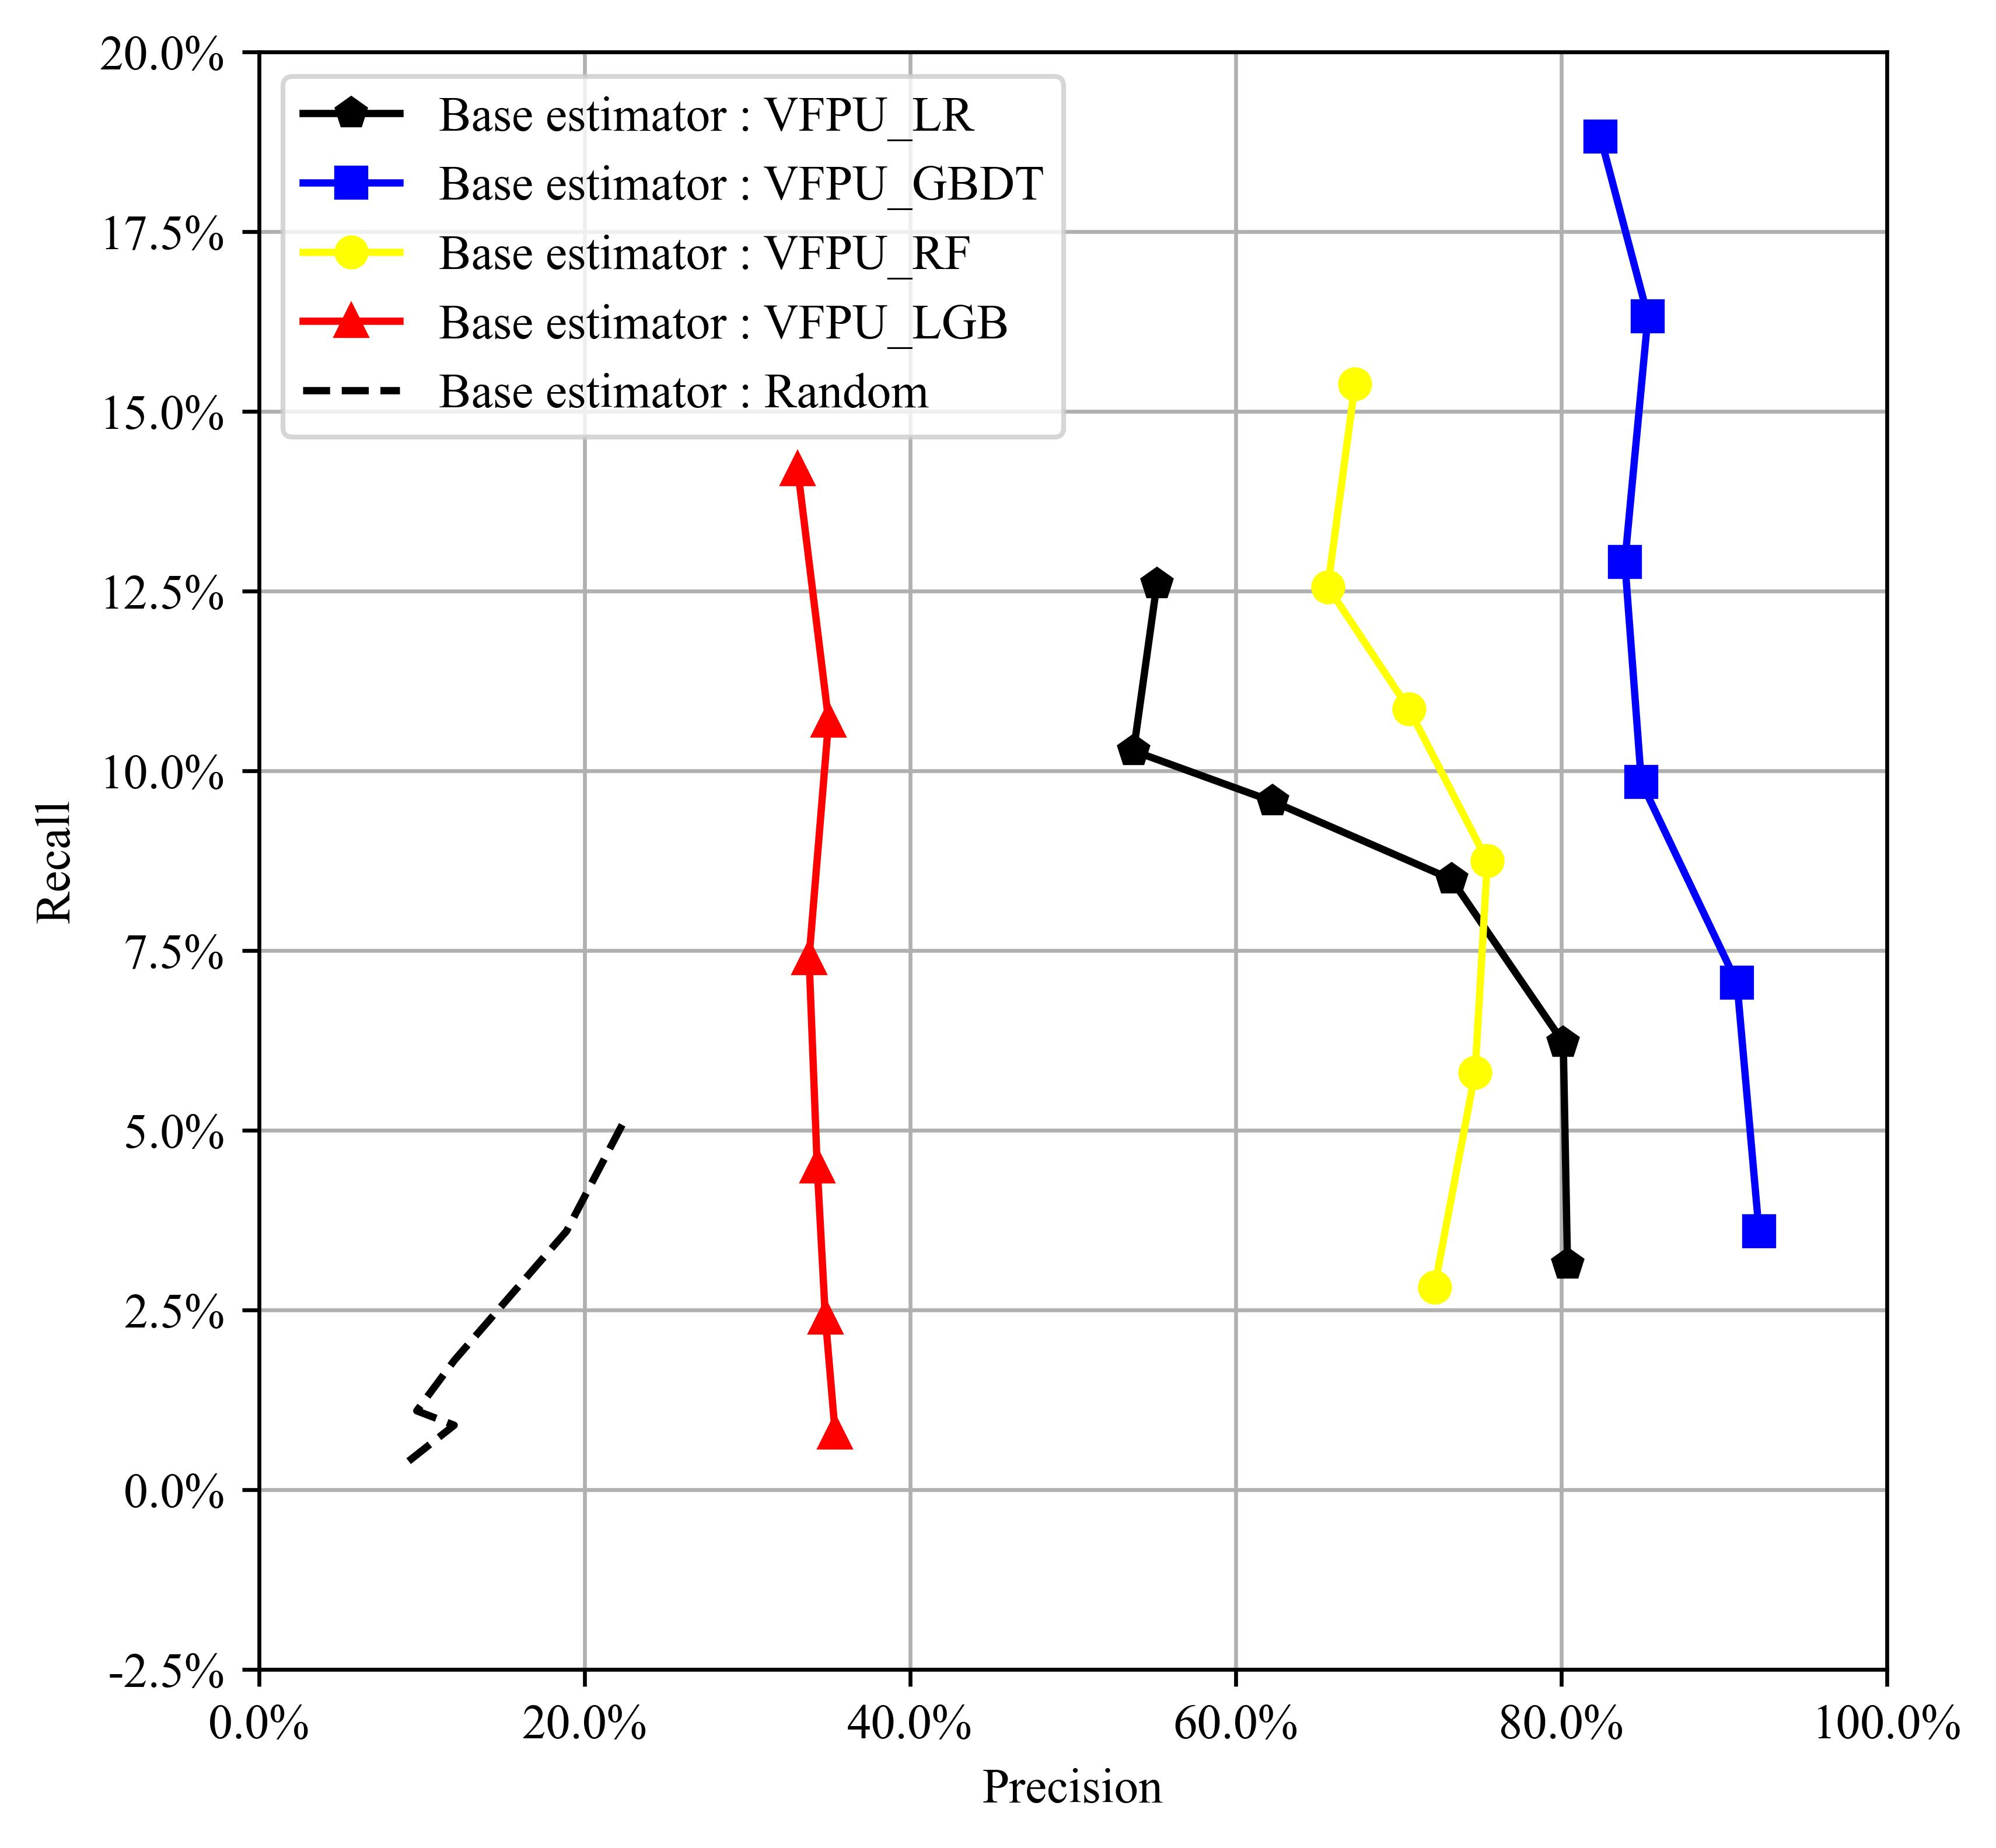
\includegraphics[width=0.45\textwidth,height=5.1cm]{chapters/imgs/Figure 4 (4) in JEPG format}}
    \begin{itemize}[leftmargin=1.6cm,rightmargin=1.6cm]
        \item[\quad] \bicaption[\xiaosi 不同基学器在不同可靠正样本数量下的性能]
        {\centering \songti \wuhao 不同基学器在不同可靠正样本数量下的性能:(a)精度;(b)召回率;(c)F-score;(d)精度-召回率(Census 数据集)}
        {\centering \wuhao Performance of Different Base Estimators with Varying Reliable Positive Samples: (a) Precision; (b) Recall; (c) F-score; (d) Precision-Recall (The Adult Census Dataset)}
    \end{itemize}
    \label{RQ2.3}
\end{figure}










\subsection{表}
% \vspace{0.1cm}  % 添加0.1厘米的垂直空间
% 
% \begin{table}[h]  % 开始表格环境,h表示尽量将表格放在当前位置
% 	\renewcommand{\arraystretch}{1.5}  % 设置表格行距为1.5倍
% 	\centering  % 表格居中
% 	\bicaption[\xiaosi 电流类型对效率的影响]{\wuhao 电流类型对效率的影响}{\wuhao Current type impact on efficiency}  % 双语标题,方括号内是目录中显示的标题(小四号字),第一个花括号内是中文标题(五号字),第二个花括号内是英文标题(五号字)
% 	\begin{tabular}{p{3cm}p{3cm}p{3cm}p{3cm}}  % 开始表格内容,定义4列,每列宽度为3厘米,p表示允许文本自动换行
% 		\toprule[1.5pt]  % 顶部粗线,粗细为1.5pt
% 		\makecell[c]{\songti\wuhao 电流类型}&\makecell[c]{\songti\wuhao A}&\makecell[c]{\songti\wuhao B}&\makecell[c]{\songti\wuhao C}\\  % 表头行,\makecell[c]表示单元格内容居中,\songti表示宋体,\wuhao表示五号字
% 		\hline  % 普通横线
% 		\makecell[c]{\wuhao aaa}&\makecell[c]{\wuhao aa1}&\makecell[c]{\wuhao bb1}&\makecell[c]{\wuhao cc1}\\  % 数据行,格式同上
% 		\bottomrule[1.5pt]  % 底部粗线,粗细为1.5pt
% 	\end{tabular}
%    \label{tab:3.1}  % 表格标签,用于交叉引用	
% \end{table}
%
% \vspace{-0.1cm}  % 调整表格与下文的间距












% \usepackage{diagbox}
% \usepackage{multirow}


\begin{table}
	\centering
	\bicaption[\xiaosi 不同半监督方法的准确推荐百分比(纵向联邦)]{\wuhao 不同半监督方法的准确推荐百分比(纵向联邦)}{\wuhao Accurate recommendations  of semi-supervised methods (in VFL)}
	\label{RQ3.2}
	\resizebox{\textwidth}{!}{
		% 整体使用 {\songti \wuhao ...} 包裹表格内容
		{\songti \wuhao
	\begin{tabular}{llllllllllll} 
	\hline
	\multicolumn{2}{\diagbox{{Datasets \& Methods}{$num$}}}        & 100              & 400              & 700              & 1000             & 1300             & 1600             & 1900             & 2100             & 2400             & runtime(s)         \\ 
	\hline
	\multirow{4}{*}{Bank}   & VF\_GBDT                & 7.00\%           & 5.30\%           & 5.30\%           & 5.00\%           & 4.70\%           & 5.20\%           & 5.10\%           & 5.00\%           & 4.80\%           & 10673.81           \\
							& VF\_Bagging GBDT        & 17.00\%          & 21.80\%          & 18.90\%          & 19.30\%          & 19.70\%          & 19.80\%          & 20.30\%          & 20.70\%          & 20.80\%          & 15069.88           \\
							& VF\_2Step GBDT          & 4.00\%           & 3.30\%           & 3.60\%           & 4.60\%           & 5.30\%           & 5.10\%           & 5.40\%           & 6.50\%           & 7.40\%           & 44030.4            \\
							& VFPU\_GBDT (Our Method) & \textbf{74.00\%} & \textbf{64.00\%} & \textbf{63.10\%} & \textbf{62.00\%} & \textbf{59.00\%} & \textbf{56.90\%} & \textbf{54.20\%} & \textbf{53.20\%} & \textbf{52.30\%} & \textbf{106922.2}  \\ 
	\hline
	\multirow{4}{*}{Credit} & VF\_GBDT                & 18.00\%          & 22.50\%          & 22.60\%          & 22.50\%          & 22.10\%          & 21.80\%          & 21.40\%          & 21.60\%          & 22.30\%          & 12025.47           \\
							& VF Bagging GBDT         & 32.00\%          & 27.50\%          & 23.90\%          & 23.60\%          & 23.50\%          & 23.40\%          & 23.30\%          & 22.30\%          & 22.00\%          & 15791.59           \\
							& VF\_2Step GBDT          & 24.00\%          & 26.30\%          & 25.40\%          & 23.90\%          & 23.70\%          & 23.10\%          & 22.30\%          & 22.30\%          & 22.00\%          & 46954.19           \\
							& VFPU\_GBDT (Our Method) & \textbf{44.00\%} & \textbf{50.25\%} & \textbf{48.86\%} & \textbf{46.50\%} & \textbf{44.85\%} & \textbf{41.88\%} & \textbf{39.47\%} & \textbf{38.33\%} & \textbf{37.43\%} & \textbf{107075.9}  \\ 
	\hline
	\multirow{4}{*}{Census} & VF\_GBDT                & 19.00\%          & 24.50\%          & 25.40\%          & 24.20\%          & 23.90\%          & 23.60\%          & 23.10\%          & 22.90\%          & 22.80\%          & 11581.47           \\
							& VF\_Bagging GBDT        & 13.00\%          & 18.00\%          & 19.90\%          & 21.10\%          & 22.30\%          & 23.30\%          & 23.20\%          & 23.20\%          & 23.90\%          & 15987.59           \\
							& VF\_2Step GBDT          & 25.00\%          & 23.30\%          & 23.10\%          & 23.40\%          & 24.30\%          & 24.10\%          & 24.60\%          & 25.00\%          & 25.60\%          & 46808.19           \\
							& VFPU\_GBDT (Our Method) & \textbf{98.00\%} & \textbf{99.00\%} & \textbf{98.71\%} & \textbf{98.70\%} & \textbf{94.23\%} & \textbf{87.25\%} & \textbf{80.53\%} & \textbf{76.05\%} & \textbf{72.74\%} & \textbf{107089.9}  \\
	\hline
	\end{tabular}
		}
	}
\end{table}







\subsection{图}
下面给出图片示例:

%调整图片与上方文字之间的间距
%\vspace{-0.1cm}

\begin{figure}[h]
		\centering 
		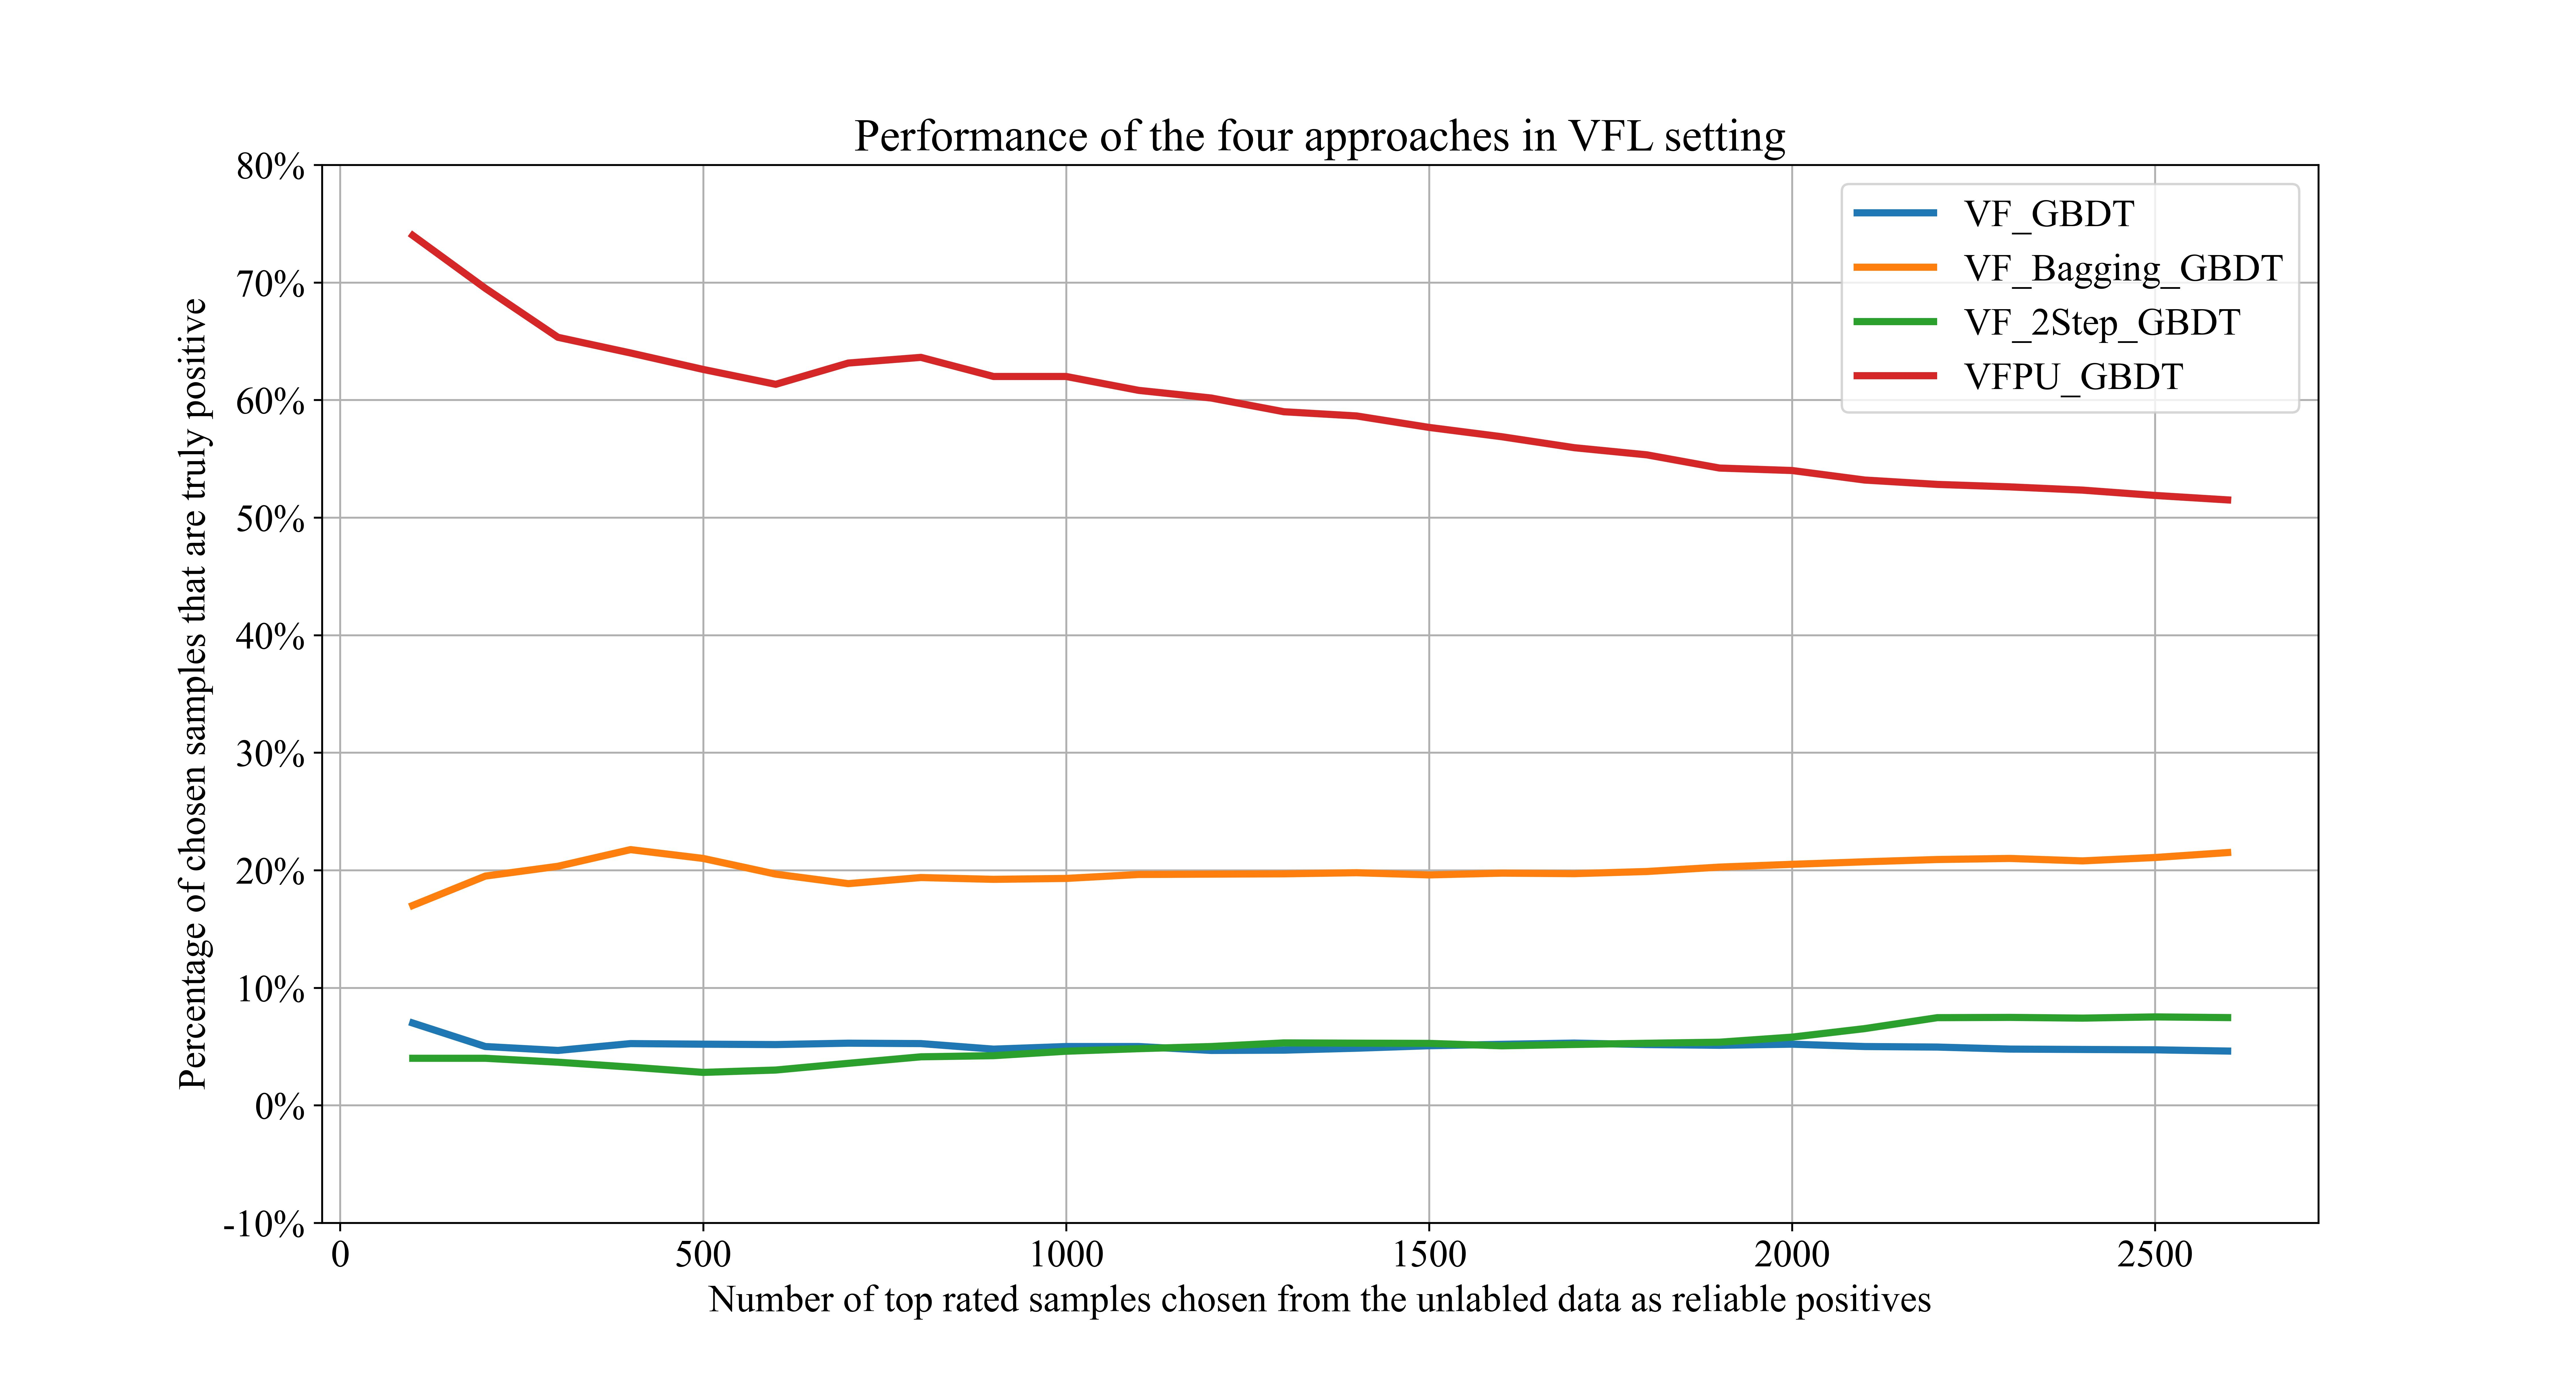
\includegraphics[width=10.9\textwidth]{chapters/imgs/Figure 5 in JPEG format}
	    \bicaption[\xiaosi 不同半监督方法在纵向联邦学习(VFL)中的准确推荐百分比]
		{\wuhao 不同半监督方法在纵向联邦学习(VFL)中的准确推荐百分比(Bamk 数据集)}
		{\wuhao The accurate recommendations percentage by Different Semi-supervised Methods in VFL (The Bank Marketing Dataset)}
	   	 \label{fig:GBDT}
\end{figure}

%调整图片与下方文字之间的间距
%\vspace{-0.35cm}




\begin{figure}[!htbp]
	\centering
	\captionsetup{size=footnotesize}
	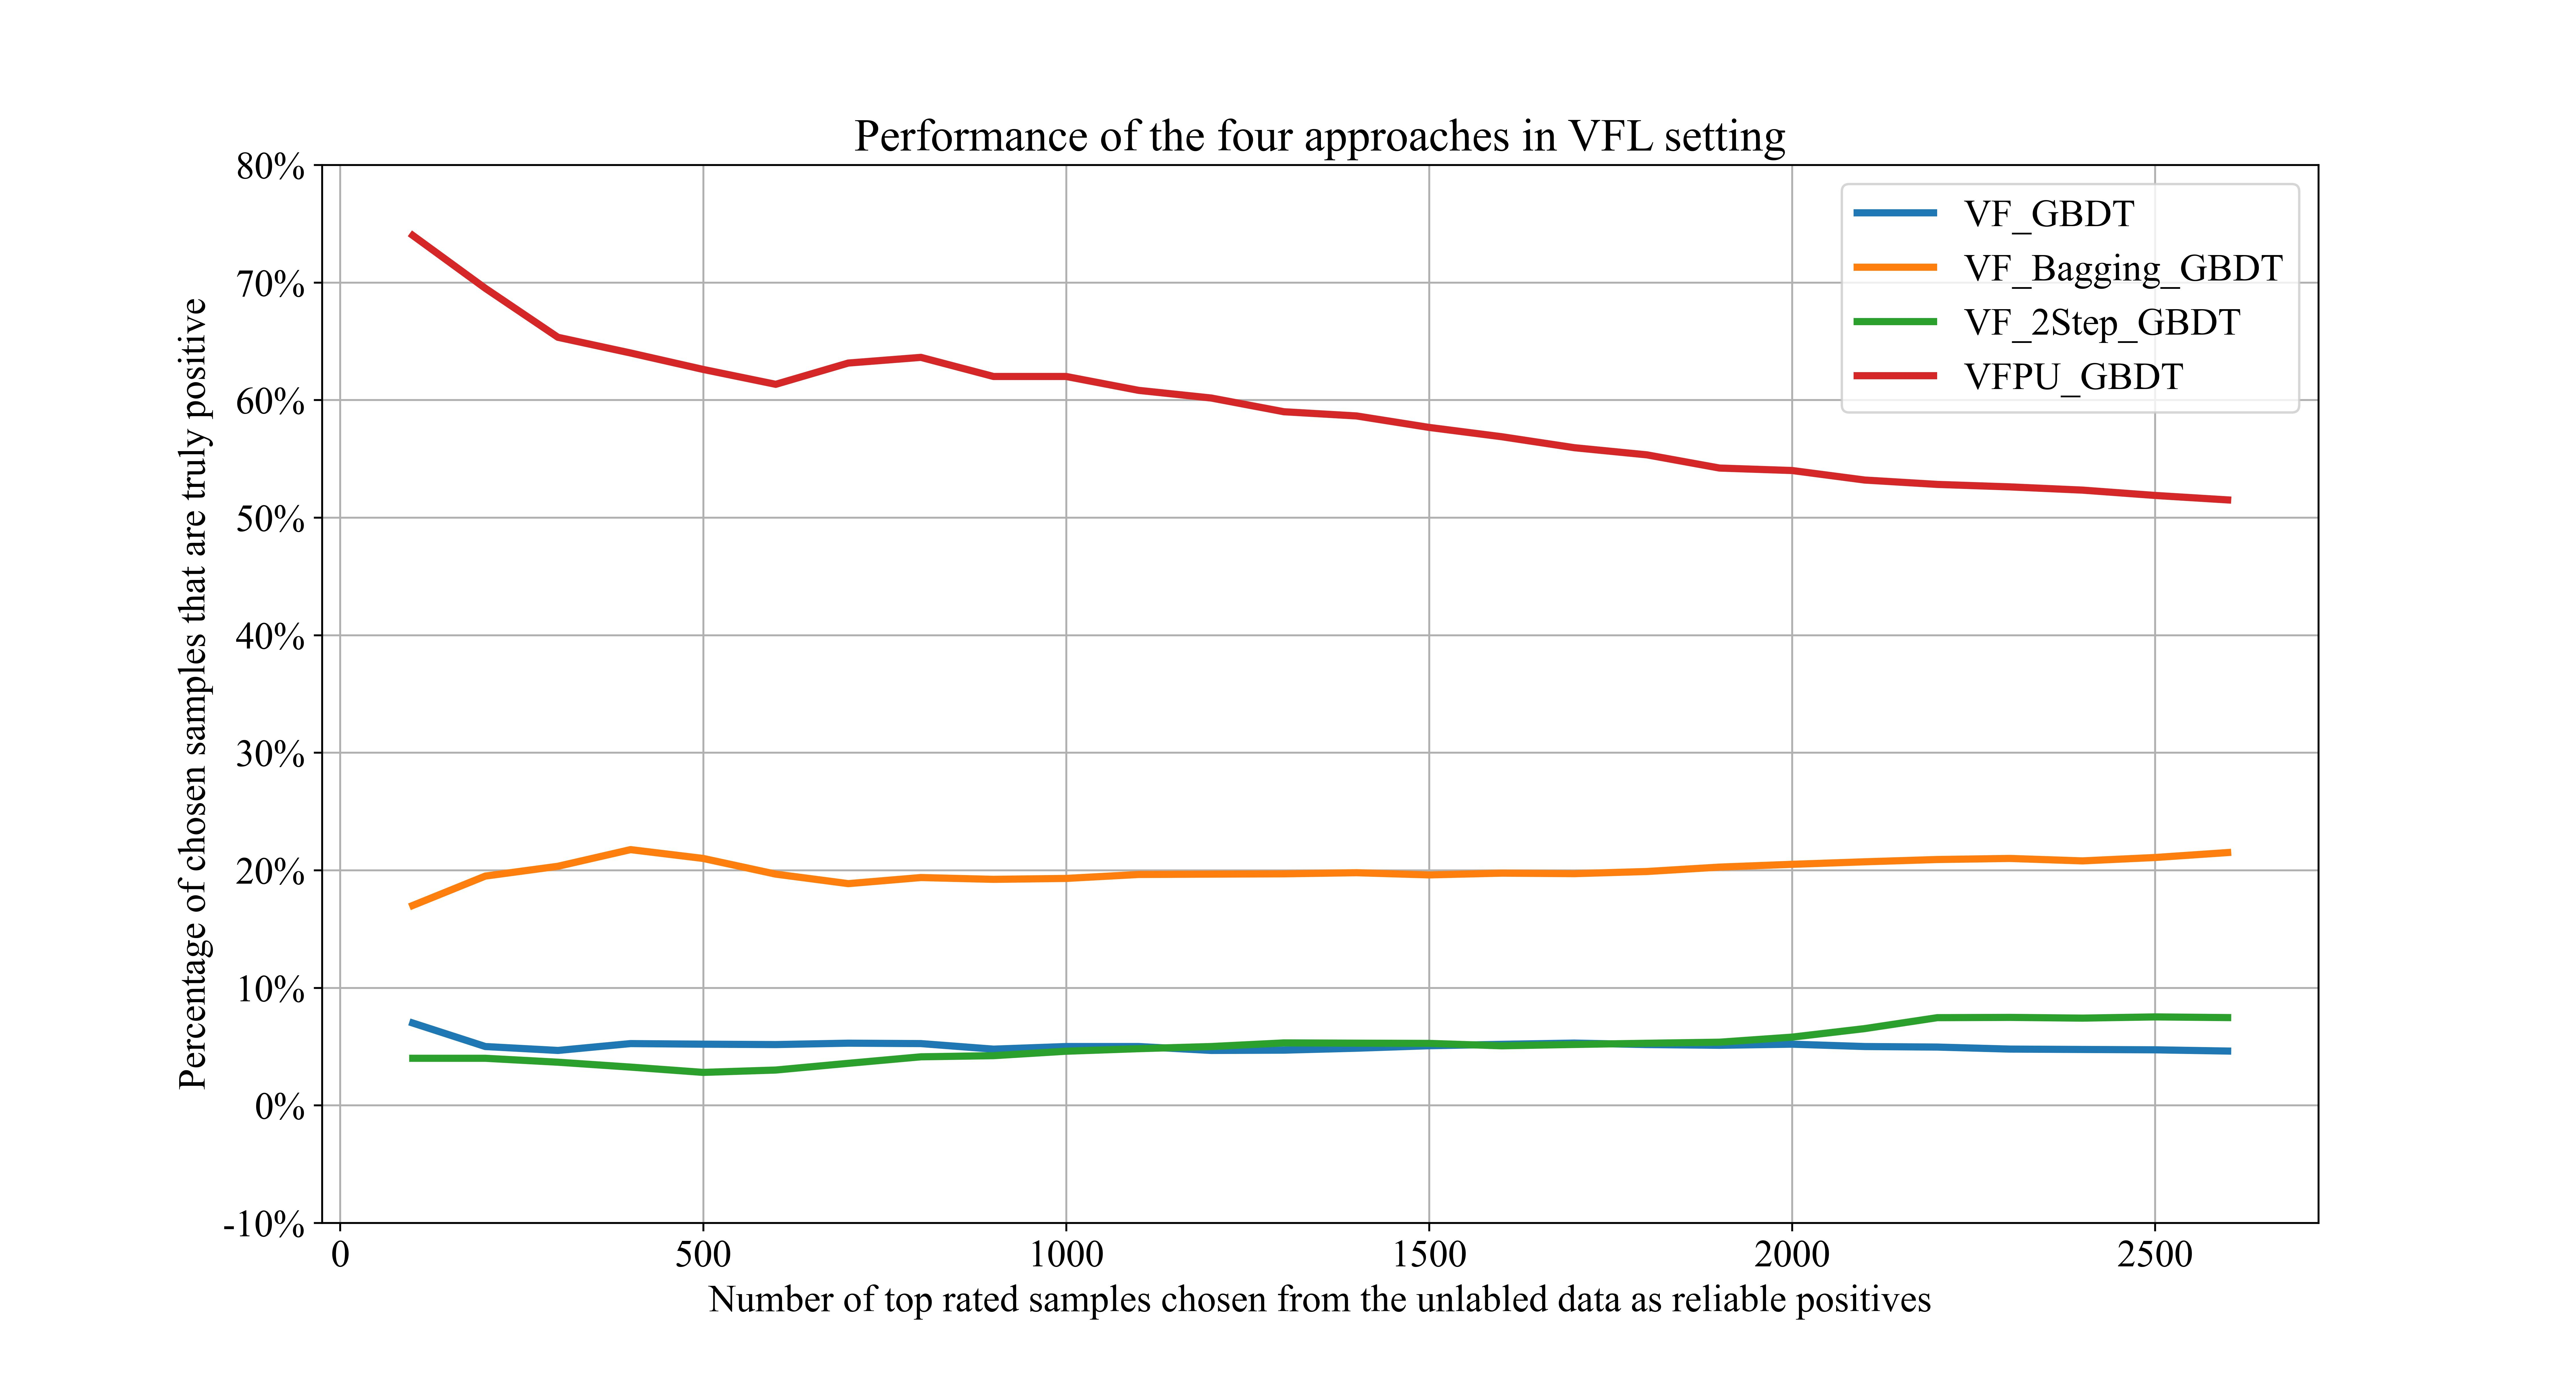
\includegraphics[width=0.9\textwidth,height=9cm]{chapters/imgs/Figure 5 in JPEG format}
	\caption{The accurate recommendations percentage by Different Semi-supervised Methods in VFL (The Banking Marketing Dataset)}
	\label{fig:GBDT}
\end{figure}







% \usepackage{multirow}


\begin{table}
	\centering
	\bicaption[\xiaosi 不同半监督方法的准确推荐百分比(无联邦)]{\wuhao 不同半监督方法的准确推荐百分比(无联邦)}{\wuhao The accurate recommendations percentage by different semi-supervised methods (without federation)}
	\label{RQ3.1}
	\begin{tabular}{llccccccccc} 
	\hline
	\multicolumn{2}{l}{\diagbox{{Datasets \& Methods}{$num$}}}                                        & 100              & 400              & 700              & 1000             & 1300             & 1600             & 1900             & 2100             & 2400              \\ 
	\hline
	\multirow{10}{*}{Bank}   & MixMatch                         & 32.81\%          & 32.50\%          & 31.25\%          & 27.97\%          & 24.85\%          & 24.53\%          & 20.31\%          & 13.44\%          & 12.03\%           \\
							 & FixMatch                         & 27.81\%          & 27.03\%          & 25.47\%          & 25.16\%          & 24.07\%          & 13.60\%          & 13.28\%          & 12.66\%          & 12.50\%           \\
							 & CoMatch                          & 31.56\%          & 27.82\%          & 24.85\%          & 24.69\%          & 24.07\%          & 18.13\%          & 17.19\%          & 12.50\%          & 12.03\%           \\
							 & AdaMatch                         & 33.56\%          & 32.97\%          & 30.50\%          & 27.69\%          & 25.78\%          & 22.50\%          & 20.63\%          & 18.13\%          & 17.19\%           \\
							 & SoftMatch                        & 32.81\%          & 31.88\%          & 31.56\%          & 25.16\%          & 24.53\%          & 21.88\%          & 19.38\%          & 17.19\%          & 12.50\%           \\
							 & \_GBDT                           & 53.65\%          & 50.03\%          & 47.00\%          & 40.20\%          & 33.62\%          & 32.64\%          & 28.99\%          & 29.17\%          & 29.33\%           \\
							 & Bagging\_GBDT                    & 42.74\%          & 41.74\%          & 33.46\%          & 29.83\%          & 28.22\%          & 34.65\%          & 31.67\%          & 27.03\%          & 26.00\%           \\
							 & 2Step\_GBDT                      & 49.79\%          & 46.66\%          & 42.79\%          & 34.93\%          & 29.72\%          & 33.88\%          & 33.38\%          & 31.30\%          & 26.85\%           \\
							 & Pseudo-Labelling                 & 33.30\%          & 22.20\%          & 22.00\%          & 20.90\%          & 21.80\%          & 22.20\%          & 24.10\%          & 23.00\%          & 22.70\%           \\
							 & No\_Fed\_VFPU\_GBDT (Our Method) & \textbf{77.00\%} & \textbf{68.25\%} & \textbf{66.86\%} & \textbf{63.80\%} & \textbf{59.62\%} & \textbf{57.63\%} & \textbf{54.26\%} & \textbf{53.95\%} & \textbf{52.38\%}  \\ 
	\hline
	\multirow{10}{*}{Credit} & MixMatch                         & 29.29\%          & 25.75\%          & 25.34\%          & 25.34\%          & 24.09\%          & 24.09\%          & 23.88\%          & 23.47\%          & 21.18\%           \\
							 & FixMatch                         & 27.00\%          & 25.55\%          & 25.34\%          & 24.30\%          & 23.88\%          & 23.47\%          & 22.85\%          & 22.43\%          & 21.39\%           \\
							 & CoMatch                          & 26.79\%          & 25.75\%          & 25.55\%          & 24.92\%          & 24.09\%          & 23.88\%          & 23.47\%          & 22.85\%          & 21.18\%           \\
							 & AdaMatch                         & 26.79\%          & 26.79\%          & 25.34\%          & 25.13\%          & 25.13\%          & 24.09\%          & 22.85\%          & 22.63\%          & 21.18\%           \\
							 & SoftMatch                        & 26.38\%          & 25.55\%          & 24.09\%          & 23.88\%          & 23.47\%          & 22.85\%          & 22.43\%          & 21.18\%          & 20.97\%           \\
							 & \_GBDT                           & 42.80\%          & 38.21\%          & 34.62\%          & 30.67\%          & 31.56\%          & 29.30\%          & 29.89\%          & 28.65\%          & 25.43\%           \\
							 & Bagging\_GBDT                    & 42.74\%          & 32.86\%          & 30.40\%          & 26.72\%          & 25.52\%          & 27.48\%          & 26.17\%          & 26.91\%          & 24.55\%           \\
							 & 2Step\_GBDT                      & 42.74\%          & 39.50\%          & 33.29\%          & 30.17\%          & 31.77\%          & 31.97\%          & 26.24\%          & 27.57\%          & 26.00\%           \\
							 & Pseudo-Labelling                 & 38.40\%          & 37.00\%          & 32.50\%          & 32.30\%          & 30.90\%          & 30.30\%          & 29.20\%          & 28.40\%          & 27.30\%           \\
							 & No\_Fed\_VFPU\_GBDT (Our Method) & \textbf{51.25\%} & \textbf{50.83\%} & \textbf{50.14\%} & \textbf{48.50\%} & \textbf{47.69\%} & \textbf{45.88\%} & \textbf{41.82\%} & \textbf{40.82\%} & \textbf{39.82\%}  \\ 
	\hline
	\multirow{10}{*}{Census} & MixMatch                         & 37.72\%          & 37.06\%          & 36.39\%          & 35.94\%          & 36.05\%          & 35.49\%          & 34.15\%          & 32.81\%          & 32.59\%           \\
							 & FixMatch                         & 38.84\%          & 38.61\%          & 37.28\%          & 37.06\%          & 36.39\%          & 35.71\%          & 34.38\%          & 33.93\%          & 32.36\%           \\
							 & CoMatch                          & 37.18\%          & 36.51\%          & 34.06\%          & 33.39\%          & 32.97\%          & 32.49\%          & 31.38\%          & 31.38\%          & 31.38\%           \\
							 & AdaMatch                         & 38.39\%          & 38.39\%          & 37.50\%          & 37.28\%          & 36.24\%          & 35.81\%          & 35.49\%          & 34.38\%          & 33.93\%           \\
							 & SoftMatch                        & 38.84\%          & 37.28\%          & 35.94\%          & 35.86\%          & 35.04\%          & 34.15\%          & 33.93\%          & 32.81\%          & 29.91\%           \\
							 & \_GBDT                           & 64.00\%          & 64.00\%          & 61.00\%          & 64.00\%          & 58.00\%          & 57.00\%          & 54.00\%          & 51.00\%          & 54.00\%           \\
							 & Bagging\_GBDT                    & 68.00\%          & 58.00\%          & 59.00\%          & 55.00\%          & 54.00\%          & 49.00\%          & 52.00\%          & 48.00\%          & 51.00\%           \\
							 & 2Step\_GBDT                      & 66.00\%          & 68.00\%          & 63.00\%          & 62.00\%          & 56.00\%          & 58.00\%          & 51.00\%          & 52.00\%          & 53.00\%           \\
							 & Pseudo-Labelling                 & 42.90\%          & 39.70\%          & 29.30\%          & 39.90\%          & 28.40\%          & 44.50\%          & 41.40\%          & 37.30\%          & 45.30\%           \\
							 & No\_Fed\_VFPU\_GBDT (Our Method) & \textbf{99.00\%} & \textbf{99.25\%} & \textbf{99.43\%} & \textbf{99.00\%} & \textbf{94.57\%} & \textbf{88.50\%} & \textbf{84.08\%} & \textbf{80.08\%} & \textbf{75.08\%}  \\
	\hline
	\end{tabular}
\end{table}




